\PassOptionsToPackage{table,dvipsnames}{xcolor}
\documentclass[nols,nobib]{tufte-book}

%%% peeragogy-shell compatibility

%\usepackage{fontspec}

\setmainfont[Mapping= tex-text,
     SmallCapsFont={Linux Libertine O},   
     SmallCapsFeatures= {Color=FFFFFF, RawFeature={+smcp,-hlig,-dlig}},   
     BoldFont={Linux Biolinum O},   
%     BoldFeatures={Color = FFFFFF,SmallCapsFont={Linux Libertine Capitals O Bold},%
%       SmallCapsFeatures = { Color=FFFFFF,   RawFeature={+smcp,+hlig,+dlig}} },  
     ItalicFont={Linux Libertine O},   
     ItalicFeatures={Color = FFFFFF,  %
       SmallCapsFont={Linux Libertine O}, %
       SmallCapsFeatures = {Color=FFFFFF,
                            Ligatures={NoCommon}},
                            Numbers=OldStyle},
     BoldItalicFont={Linux Libertine O},
     BoldItalicFeatures={ Color = FFFFFF, %
      SmallCapsFont={Linux Libertine O},  %
      SmallCapsFeatures = { Color=FFFFFF,
                            RawFeature={+smcp,-hlig,-dlig}}} ]{Linux Libertine O} 

\newfontfamily{\icon}{Symbola}
\newfontfamily{\mapicon}{map-icons}
%\newfontfamily{\material}{materialdesignicons-webfont.ttf}

\newcommand\Sthreshold{{\icon \symbol{"1F6AA}}}
\newcommand\Strust{{\icon \symbol{"1F44B}}}
\newcommand\Svariety{{\icon \symbol{"2A3B}}}
\newcommand\Sclarity{{\icon \symbol{"26EF}}}
\newcommand\Scoherence{{\icon \symbol{"2699}}}
\newcommand\Sderivative{{\icon \symbol{"2207}}}
\newcommand\Ssensemaking{{\icon \symbol{"1F44D}}}
\newcommand\Ssharing{{\icon \symbol{"1F4C8}}}
\newcommand\Santifragility{{\icon \symbol{"1F3CA}}}
\newcommand\Sindependence{{\icon \symbol{"1F527}}}
\newcommand\Sdifferentiation{{\mapicon \symbol{"E86F}}} % swing
\newcommand\Sdifficulty{{\mapicon \symbol{"4DC2}}}
\newcommand\Sinertia{{\mapicon \symbol{"1F3CB}}}
\newcommand\Sentropy{{\icon \symbol{"1F739}}}
\newcommand\Sinterface{{\icon \symbol{"1F6CE}}}
\newcommand\Sfamiliar{{\icon \symbol{"1D318}}}
\newcommand\Sequity{{\icon \symbol{"1F310}}}
\newcommand\Sindividuation{{\mapicon \symbol{"E86F}}}
\newcommand\Smutuality{{\mapicon \symbol{"1F450}}}
\newcommand\Sattention{{\icon \symbol{"1F92B}}}
\newcommand\Sinterest{{\mapicon \symbol{"E8A7}}}
\newcommand\Smeaning{{\mapicon \symbol{"E873}}}

\providecommand{\tightlist}{%
  \setlength{\itemsep}{0pt}\setlength{\parskip}{0pt}}

\usepackage[style=verbose, autocite=footnote, backend=biber, doi=false,url=false,isbn=false]{biblatex}
\addbibresource{pattern-catalog-bib.bib}

\renewcommand{\cite}[2][0pt]{\sidenote{\fullcite{#2}}}

\newcommand{\patternname}[1]{\hyperref[sec:#1]{{\sc #1}}}
\newcommand{\patternnameext}[1]{{\sc #1}}
\newcommand{\patternnameplural}[1]{\hyperref[sec:#1]{{\sc #1s}}}
\newcommand{\patternnameposesssive}[1]{\hyperref[sec:#1]{{\sc #1's}}}

\usepackage{tikz}
\usetikzlibrary{calc}
\usetikzlibrary{positioning,backgrounds,fit,arrows,arrows.meta,shapes,shadows}
\usetikzlibrary{shapes.multipart}
\usetikzlibrary{intersections}
\usepackage{pgflibraryarrows}

\usepackage{array}
\usepackage{tabularx}

%%% Bibliography items

\newbibmacro{string+doiurlisbn}[1]{%
  \iffieldundef{doi}{%
    \iffieldundef{url}{%
      \iffieldundef{isbn}{%
        \iffieldundef{issn}{%
          #1%
        }{%
          \href{http://books.google.com/books?vid=ISSN\thefield{issn}}{#1}%
        }%
      }{%
        \href{http://books.google.com/books?vid=ISBN\thefield{isbn}}{#1}%
      }%
    }{%
      \href{\thefield{url}}{#1}%
    }%
  }{%
    \href{http://dx.doi.org/\thefield{doi}}{#1}%
  }%
}

\DeclareFieldFormat{title}{\usebibmacro{string+doiurlisbn}{\mkbibemph{#1}}}
\DeclareFieldFormat[article,incollection]{title}%
{\usebibmacro{string+doiurlisbn}{\mkbibquote{#1}}}
                   
%%% Compatibility

\let\sc\scshape
\renewcommand\smallcaps[1]{{\sc #1}}

%%% Tufte setup

\hypersetup{colorlinks}% uncomment this line if you prefer colored hyperlinks (e.g., for onscreen viewing)

%%
% Book metadata
\title{The Peeragogy Handbook}
\author[The Tufte-LaTeX Developers]{\emph{Editors}\\
{\small Joseph Corneli, Charles Jeffrey Danoff, Paola Ricaurte,}\\
{\small Charlotte Pierce, and Lisa Snow MacDonald} \\[.25in]}
\publisher{Pierce Press \& Pub Dom Ed \Sdifferentiation}

%%
% If they're installed, use Bergamo and Chantilly from www.fontsite.com.
% They're clones of Bembo and Gill Sans, respectively.
%\IfFileExists{bergamo.sty}{\usepackage[osf]{bergamo}}{}% Bembo
%\IfFileExists{chantill.sty}{\usepackage{chantill}}{}% Gill Sans

%\usepackage{microtype}

%%
% Just some sample text
\usepackage{lipsum}

%%
% For nicely typeset tabular material
\usepackage{booktabs}

%%
% For graphics / images
\usepackage{graphicx}
\setkeys{Gin}{width=\linewidth,totalheight=\textheight,keepaspectratio}
\graphicspath{{graphics/}}

% The fancyvrb package lets us customize the formatting of verbatim
% environments.  We use a slightly smaller font.
\usepackage{fancyvrb}
\fvset{fontsize=\normalsize}

%%
% Prints argument within hanging parentheses (i.e., parentheses that take
% up no horizontal space).  Useful in tabular environments.
\newcommand{\hangp}[1]{\makebox[0pt][r]{(}#1\makebox[0pt][l]{)}}

%%
% Prints an asterisk that takes up no horizontal space.
% Useful in tabular environments.
\newcommand{\hangstar}{\makebox[0pt][l]{*}}

%%
% Prints a trailing space in a smart way.
\usepackage{xspace}


\newcommand{\TL}{Tufte-\LaTeX\xspace}

% Prints the month name (e.g., January) and the year (e.g., 2008)
\newcommand{\monthyear}{%
  \ifcase\month\or January\or February\or March\or April\or May\or June\or
  July\or August\or September\or October\or November\or
  December\fi\space\number\year
}


% Prints an epigraph and speaker in sans serif, all-caps type.
\newcommand{\openepigraph}[2]{%
  %\sffamily\fontsize{14}{16}\selectfont
  \begin{fullwidth}
  \sffamily\large
  \begin{doublespace}
  \noindent\allcaps{#1}\\% epigraph
  \noindent\allcaps{#2}% author
  \end{doublespace}
  \end{fullwidth}
}

% Inserts a blank page
\newcommand{\blankpage}{\newpage\hbox{}\thispagestyle{empty}\newpage}

\usepackage{units}

% Typesets the font size, leading, and measure in the form of 10/12x26 pc.
\newcommand{\measure}[3]{#1/#2$\times$\unit[#3]{pc}}

% Macros for typesetting the documentation
\newcommand{\hlred}[1]{\textcolor{Maroon}{#1}}% prints in red
\newcommand{\hangleft}[1]{\makebox[0pt][r]{#1}}
\newcommand{\hairsp}{\hspace{1pt}}% hair space
\newcommand{\hquad}{\hskip0.5em\relax}% half quad space
\newcommand{\TODO}{\textcolor{red}{\bf TODO!}\xspace}
\newcommand{\ie}{\textit{i.\hairsp{}e.}\xspace}
\newcommand{\eg}{\textit{e.\hairsp{}g.}\xspace}
\newcommand{\na}{\quad--}% used in tables for N/A cells
\providecommand{\XeLaTeX}{X\lower.5ex\hbox{\kern-0.15em\reflectbox{E}}\kern-0.1em\LaTeX}
\newcommand{\tXeLaTeX}{\XeLaTeX\index{XeLaTeX@\protect\XeLaTeX}}
% \index{\texttt{\textbackslash xyz}@\hangleft{\texttt{\textbackslash}}\texttt{xyz}}
\newcommand{\tuftebs}{\symbol{'134}}% a backslash in tt type in OT1/T1
\newcommand{\doccmdnoindex}[2][]{\texttt{\tuftebs#2}}% command name -- adds backslash automatically (and doesn't add cmd to the index)
\newcommand{\doccmddef}[2][]{%
  \hlred{\texttt{\tuftebs#2}}\label{cmd:#2}%
  \ifthenelse{\isempty{#1}}%
    {% add the command to the index
      \index{#2 command@\protect\hangleft{\texttt{\tuftebs}}\texttt{#2}}% command name
    }%
    {% add the command and package to the index
      \index{#2 command@\protect\hangleft{\texttt{\tuftebs}}\texttt{#2} (\texttt{#1} package)}% command name
      \index{#1 package@\texttt{#1} package}\index{packages!#1@\texttt{#1}}% package name
    }%
}% command name -- adds backslash automatically
\newcommand{\doccmd}[2][]{%
  \texttt{\tuftebs#2}%
  \ifthenelse{\isempty{#1}}%
    {% add the command to the index
      \index{#2 command@\protect\hangleft{\texttt{\tuftebs}}\texttt{#2}}% command name
    }%
    {% add the command and package to the index
      \index{#2 command@\protect\hangleft{\texttt{\tuftebs}}\texttt{#2} (\texttt{#1} package)}% command name
      \index{#1 package@\texttt{#1} package}\index{packages!#1@\texttt{#1}}% package name
    }%
}% command name -- adds backslash automatically
\newcommand{\docopt}[1]{\ensuremath{\langle}\textrm{\textit{#1}}\ensuremath{\rangle}}% optional command argument
\newcommand{\docarg}[1]{\textrm{\textit{#1}}}% (required) command argument
\newenvironment{docspec}{\begin{quotation}\ttfamily\parskip0pt\parindent0pt\ignorespaces}{\end{quotation}}% command specification environment
\newcommand{\docenv}[1]{\texttt{#1}\index{#1 environment@\texttt{#1} environment}\index{environments!#1@\texttt{#1}}}% environment name
\newcommand{\docenvdef}[1]{\hlred{\texttt{#1}}\label{env:#1}\index{#1 environment@\texttt{#1} environment}\index{environments!#1@\texttt{#1}}}% environment name
\newcommand{\docpkg}[1]{\texttt{#1}\index{#1 package@\texttt{#1} package}\index{packages!#1@\texttt{#1}}}% package name
\newcommand{\doccls}[1]{\texttt{#1}}% document class name
\newcommand{\docclsopt}[1]{\texttt{#1}\index{#1 class option@\texttt{#1} class option}\index{class options!#1@\texttt{#1}}}% document class option name
\newcommand{\docclsoptdef}[1]{\hlred{\texttt{#1}}\label{clsopt:#1}\index{#1 class option@\texttt{#1} class option}\index{class options!#1@\texttt{#1}}}% document class option name defined
\newcommand{\docmsg}[2]{\bigskip\begin{fullwidth}\noindent\ttfamily#1\end{fullwidth}\medskip\par\noindent#2}
\newcommand{\docfilehook}[2]{\texttt{#1}\index{file hooks!#2}\index{#1@\texttt{#1}}}
\newcommand{\doccounter}[1]{\texttt{#1}\index{#1 counter@\texttt{#1} counter}}

% Generates the index
\usepackage{makeidx}
\makeindex

\begin{document}

% Front matter
\frontmatter

% r.3 full title page
\maketitle

% v.4 copyright page
\newpage
\begin{fullwidth}
~\vfill
\thispagestyle{empty}
\setlength{\parindent}{0pt}
\setlength{\parskip}{\baselineskip}
Copyright \copyright\ {2012-2020} by the authors has been transferred to the Public Domain.\\[.25in]

\emph{Editorial Board}\\
{\small Joseph Corneli, Charles Jeffrey Danoff, Paola Ricaurte,}\\
{\small Charlotte Pierce, and Lisa Snow MacDonald} \\[.25in]

\emph{Contributors} \\
{\small Bryan Alexander, Paul Allison, Elisa Armend\'ariz,} \\
{\small R\'egis Barondeau, George Brett, Doug Breitbart,}\\ 
{\small Suz Burroughs, Teryl Cartwright, Jay Cross,}\\
{\small Karen Beukema Einstein, Julian Elve, Mar\'ia Fernanda Arenas,}\\
{\small James Folkestad, Kathy Gill, John Glass,} \\
{\small John Graves, Jan Herder, Matthew Herschler,} \\
{\small Gigi Johnson, Anna Keune, Kyle Larson,} \\
{\small Roland Legrand, Amanda Lyons, Dorotea Mar,} \\
{\small Christopher Tillman Neal, Ted Newcomb, Stephanie Parker,} \\
{\small Miguel \'Angel P\'erez \'Alvarez, David Preston, Laura Ritchie,} \\
{\small Verena Roberts, Stephanie Schipper, Peter Taylor,}\\
{\small Fabrizio Terzi, and Geoff Walker}\\[.25in]

\emph{Founded by}\\
{\small Howard Rheingold}\\[.25in]

\par\smallcaps{Jointly published by Pierce Press and PubDomEd.}

Layout: \smallcaps{tufte-latex.googlecode.com} (Apache License, Version 2.0)

%% \par Licensed under the Apache License, Version 2.0 (the ``License''); you may not
%% use this file except in compliance with the License. You may obtain a copy
%% of the License at \url{http://www.apache.org/licenses/LICENSE-2.0}. Unless
%% required by applicable law or agreed to in writing, software distributed
%% under the License is distributed on an \smallcaps{``AS IS'' BASIS, WITHOUT
%% WARRANTIES OR CONDITIONS OF ANY KIND}, either express or implied. See the
%% License for the specific language governing permissions and limitations
%% under the License.\index{license}

\par\textit{First printing, \monthyear}
\end{fullwidth}


% r.5 contents
\tableofcontents

\listoffigures

\listoftables

% r.9 introduction
\cleardoublepage

\phantomsection
\chapter*{Foreword}
%\pagestyle{companion}
\markboth{{\sc Foreword}}{{\sc Foreword}}
\addcontentsline{toc}{chapter}{Foreword}
%
\input{foreword.tex}
 %%%%%%%%%%%%%%%%%%%%  %%%%%%%%%%%%%%%%%%%%  %%%%%%%%%%%%%%%%%%%%

\newpage
 %%%%%%%%%%%%%%%%%%%%  %%%%%%%%%%%%%%%%%%%%  %%%%%%%%%%%%%%%%%%%%
\phantomsection
\chapter*{Preface to the Fourth Edition}
\addcontentsline{toc}{chapter}{Preface to the Fourth Edition}

%\input{preface.tex}
\emph{Add me.}

\clearpage
 %%%%%%%%%%%%%%%%%%%%  %%%%%%%%%%%%%%%%%%%%  %%%%%%%%%%%%%%%%%%%%

\mainmatter

%%% \part{Introduction} \label{intro-part} %%%%%%%%%%%%%%%%%%%%
%\pagestyle{companion}
\chapter[\textbf{Welcome!}]{Welcome to the Peeragogy Handbook}
%
\textbf{Welcome to the Peeragogy Handbook!}

This book, and accompanying website, is a resource for self-organizing
self-learners.

With YouTube, Wikipedia, search engines, free chatrooms, blogs, wikis,
and video communication, today's
\href{http://en.wikipedia.org/wiki/Self-taught\_learner}{self-learners}
have power never dreamed-of before. What does any group of self-learners
need to know in order to self-organize learning about any topic? The
Peeragogy Handbook is a volunteer-created and maintained resource for
bootstrapping peer learning.

This project seeks to empower the worldwide population of self-motivated
learners who use digital media to connect with each other, to
co-construct knowledge of how to co-learn. Co-learning is ancient; the
capacity for learning by imitation and more, to teach others what we
know, is the essence of human culture. We are human because we learn
together. Today, however, the advent of digital production media and
distribution/communication networks has raised the power and potential
of co-learning to a new level.

If you want to learn how to fix a pipe, solve a partial differential
equation, write software, you are seconds away from know-how via
YouTube, Wikipedia and search engines. Access to technology and access
to knowledge, however, isn't enough. Learning is a social, active, and
ongoing process.

\begin{quote}
\emph{What does a motivated group of self-learners need to know to agree
on a subject or skill, find and qualify the best learning resources
about that topic, select and use appropriate communication media to
co-learn it?~ In particular, what do they need to know about peer
learning?}
\end{quote}

This handbook is intended to answer these questions, and in the process,
build a toolbox for co-learning.

Our experience within this project has been that flattened hierarchies
do not necessarily mean decisions go by consensus. The handbook is in
part a collaboration? and in part a collection of single-author works.
Often the lines and voices are blurred. One constant throughout the book
is our interest in making something useful. To this end, the book comes
with numerous~activities, and is available under non-restrictive legal
terms (you can reuse portions of it however you see fit it has been
given a \href{http://creativecommons.org/publicdomain/zero/1.0/}{CC Zero
1.0 Universal Public Domain Dedication}). For those who seek more
evidence-based, scholarly scaffolding for learning practices, we also
maintain a
\href{http://peeragogy.org/resources/literature-review-peeragogy/}{literature
review} of learning theories that pertain to self-organized peer
learning.

Finally, we also include instructions on
\href{http://peeragogy.org/resources/how-to-get-involved/}{how to join
us in further developing this resource}.

Sincerely, \href{http://peeragogy.org/resources/meet-the-team/}{The
Peeragogy Team}


\newpage

%% \addtocontents{toc}{%
%%  \protect\vspace{-.5cm}%
%% }
%% \includepdf[addtotoc={1,chapter,0,Workbook,chap:workbook},page={1-},offset=5mm 0mm,pagecommand={\pagestyle{companion}}]{peeragogy-workbook-insert.pdf}

\input{workbook.tex}

\chapter[\textbf{Chapter Summaries}]{Chapter Summaries}
%
\hypertarget{motivation}{%
\subsubsection{Motivation}\label{motivation}}

You might wonder why we're doing this project -- what we hope to get out
of it as volunteers, and how we think what we're doing can make a
positive difference in the world. Have a look at this chapter if you,
too, are thinking about getting involved in peeragogy, or wondering how
peeragogy can help you accelerate your learning projects.

\hypertarget{case-study-5ph1nx.}{%
\paragraph{\texorpdfstring{\emph{Case Study:
5PH1NX.}}{Case Study: 5PH1NX.}}\label{case-study-5ph1nx.}}

This example focuses on the interrelationship of pedagogy and peeragogy
in a high school English class, when students are encouraged to find and
share creative ways to learn. Explore this case study for ideas and
encouragement for your own learning adventures.

\hypertarget{peeragogy-in-practice}{%
\subsubsection{Peeragogy in Practice}\label{peeragogy-in-practice}}

Here we describe some of the interaction patterns that we've encountered
time and time again in the Peeragogy project. You can use the ideas in
this chapter as a starter-kit for your own experiments with peeragogy
right away. Sharing -- and revising -- patterns is one of the key
activities in peeragogy, so you will likely want to revisit this chapter
several times as you look through the rest of the book. Don't forget
your red pen or pencil, because you'll also want to tailor the patterns
we describe here to suit.

\hypertarget{case-study-swats.}{%
\paragraph{\texorpdfstring{\emph{Case Study:
SWATS.}}{Case Study: SWATS.}}\label{case-study-swats.}}

We present another example of peer learning in a classroom setting,
focusing on the process of improving overall student performance with
the help of a group of student experts. After describing the case study
in general terms, we then re-analyze it using our pattern tools to show
how examples like this can be integrated into our project.

\hypertarget{convening-a-group}{%
\subsubsection{Convening a Group}\label{convening-a-group}}

This chapter is about how to begin your own peeragogical project. You
can also use the ideas described here to strengthen an existing
collaboration. Simple but important questions will inspire unique
answers for you and your group. In short: who, what, when, where, why,
and how? Use this chapter to help design and critique your project's
roadmap.

\hypertarget{play-learning.}{%
\paragraph{\texorpdfstring{\emph{Play \&
Learning.}}{Play \& Learning.}}\label{play-learning.}}

What makes learning fun? Just as actors learn their roles through the
dynamic process of performance, In other words, the more we engage with
a topic, the better we learn it and the more satisfying - or fun - the
process becomes.

\hypertarget{k-12-peeragogy.}{%
\paragraph{\texorpdfstring{\emph{K-12
Peeragogy.}}{K-12 Peeragogy.}}\label{k-12-peeragogy.}}

The key to becoming a successful `connected educator-learner' involves
spending the time needed to learn how to learn and share in an open,
connected environment. Once you make the decision to enter into a
dialogue with another user, you become a connected educator/learner and
tap into the power of networks to distribute the load of learning.
Depending on their age, you can even facilitate an awareness of peer
networks among your students.

\hypertarget{p2p-self-organizing-learning-environments.}{%
\paragraph{\texorpdfstring{\emph{P2P Self-Organizing Learning
Environments.}}{P2P Self-Organizing Learning Environments.}}\label{p2p-self-organizing-learning-environments.}}

This section invites an exploration of support for self-organized
learning in global and local networks. Emergent structures can create
startling ripple effects.

\hypertarget{organizing-a-learning-context}{%
\subsubsection{Organizing a Learning
Context}\label{organizing-a-learning-context}}

Peer learning is sometimes organized in ``courses'' and sometimes in
``spaces.'' We present the results of an informal poll that reveals some
of the positive and some of the negative features of our own early
choices in this project.

\hypertarget{adding-structure-with-activities.}{%
\paragraph{\texorpdfstring{\emph{Adding Structure with
Activities.}}{Adding Structure with Activities.}}\label{adding-structure-with-activities.}}

The first rule of thumb for peer learning is: announce activities only
when you plan to take part as a fully engaged participant. Then ask a
series of questions: what is the goal, what makes it challenging, what
worked in other situations, what recipe is appropriate, what is
different about learning about this topic?

\hypertarget{student-authored-syllabus.}{%
\paragraph{\texorpdfstring{\emph{Student Authored
Syllabus.}}{Student Authored Syllabus.}}\label{student-authored-syllabus.}}

This chapter describes various methods for co-creating a curriculum. If
you're tasked with teaching an existing curriculum, you may want to
start with a smaller co-created activity; but watch out, you may find
that co-creation is habit forming.\footnote{Quick tip: if you create a
  syllabus, share it!}

\hypertarget{case-study-collaborative-explorations.}{%
\paragraph{\texorpdfstring{\emph{Case Study: Collaborative
Explorations.}}{Case Study: Collaborative Explorations.}}\label{case-study-collaborative-explorations.}}

This chapter describes collaborative peer learning among adult students
in the Master's program in Critical and Creative Thinking at University
of Massachusetts in Boston. The idea in the collaborative explorations
is to encourage individuals pursuing their own interests related to a
predetermined topic, while supporting learning of everyone in the group
through sharing and reflection. These interactions of supportive mutual
inquiry evolve the content and structure within a short time frame and
with open-ended results.

\hypertarget{cooperation}{%
\subsubsection{Cooperation}\label{cooperation}}

Sometimes omitting the figurehead empowers a group. Co-facilitation
tends to work in groups of people who gather to share common problems
and experiences. The chapter suggests several ways to co-facilitate
discussions, wiki workflows, and live online sessions. Conducting an
``after action review'' can help expose blind spots.

\hypertarget{the-workscape.}{%
\paragraph{\texorpdfstring{\emph{The
Workscape.}}{The Workscape.}}\label{the-workscape.}}

In a corporate workscape, people are free-range learners: protect the
learning environment, provide nutrients for growth, and let nature take
its course. A workscape features profiles, an activity stream, wikis,
virtual meetings, blogs, bookmarks, mobile access and a social network.

\hypertarget{participation.}{%
\paragraph{\texorpdfstring{\emph{Participation.}}{Participation.}}\label{participation.}}

Participation grows from having a community of people who learn
together, using a curriculum as a starting point to organize and trigger
engagement. Keep in mind that participation may follow the 90/9/1
principle (lurkers/editors/authors) and that people may transition
through these roles over time.

\hypertarget{designs-for-co-working.}{%
\paragraph{\texorpdfstring{\emph{Designs For
Co-Working.}}{Designs For Co-Working.}}\label{designs-for-co-working.}}

Designing a co-working platform to include significant peer learning
aspects often requires a new approach. This chapter describes the
initial steps of converting an existing online encyclopedia project into
a peer learning platform.

\hypertarget{assessment}{%
\subsubsection{Assessment}\label{assessment}}

``Usefulness'' is an appropriate metric for assessment in peeragogy,
where we're concerned with devising our own problems rather than than
the problems that have been handed down by society. We use the idea of
return on investment (the value of changes in behavior divided by the
cost of inducing the change) to assess the Peeragogy project itself, as
one example.

\hypertarget{researching-peeragogy.}{%
\paragraph{\texorpdfstring{\emph{Researching
peeragogy.}}{Researching peeragogy.}}\label{researching-peeragogy.}}

This chapter is based on a ``found manuscript'' created by one of us as
an undergraduate. It looks at the challenges that are associated with
combining the roles of student, teacher, and researcher. It shows the
relevance of peer support, and also illustrates the important factor of
time in the evolution of an idea.

\hypertarget{technologies-services-and-platforms}{%
\subsubsection{Technologies, Services, and
Platforms}\label{technologies-services-and-platforms}}

Issues of utility, choice, coaching, impact and roles attach to the wide
variety of tools and technologies available for peer learning. Keys to
selection include the features you need, what people are already using,
and the type of tool (low threshold, wide wall, high ceilings) used for
collaboration.

\hypertarget{forums.}{%
\paragraph{\texorpdfstring{\emph{Forums.}}{Forums.}}\label{forums.}}

Forums are web-based communication media that enable groups of people to
conduct organized multimedia discussions about multiple topics over a
period of time, asynchronously. A rubric for evaluating forum posts
highlights the value of drawing connections. This chapter includes tips
on selecting forum software.

\hypertarget{wiki.}{%
\paragraph{\texorpdfstring{\emph{Wiki.}}{Wiki.}}\label{wiki.}}

A wiki is a website whose users can add, modify, or delete its content
via a web browser. Pages have a feature called ``history'' which allows
users to see previous versions and roll back to them. This chapter
includes tips on how to use a wiki and select a wiki engine, with
particular attention to peer learning opportunities.

\hypertarget{real-time-meetings.}{%
\paragraph{\texorpdfstring{\emph{Real-time
meetings.}}{Real-time meetings.}}\label{real-time-meetings.}}

Web services enable broadband-connected learners to communicate in real
time via audio, video, slides, whiteboards, chat, and screen-sharing.
Possible roles for participants in real-time meetings include searchers,
contextualizers, summarizers, lexicographers, mappers, and curators.
This mode of interaction supports emergent agendas.

\hypertarget{connectivism-in-practice.}{%
\paragraph{\texorpdfstring{\emph{Connectivism in
Practice.}}{Connectivism in Practice.}}\label{connectivism-in-practice.}}

Massive Open Online Courses (MOOCs) are decentralized online learning
experiences: individuals and groups create blogs or wikis and comment on
each other's work, often with other tools helping find information.

\hypertarget{resources}{%
\subsubsection{Resources}\label{resources}}

Here we present a sample syllabus for bringing peer learning to life,
recommended reading and tips on writing for The Handbook, as well as our
Creative Commons Zero 1.0 Universal (CC0 1.0) Public Domain Dedication.


%%% \part{Motivation} \label{motivation-part} %%%%%%%%%%%%%%%%%%%%

%
\chapter[\textbf{Why we're doing this}]{Why we're doing this}
\begin{quote}
Participants must bring self-knowledge and no small measure of honesty
to the peer-learning project in order to accurately enunciate their
motivations. If everyone in your peer learning project asks ``What
brings me here?'' ``How can I contribute?'' and ``How can I contribute
more effectively?'' things will really start percolating. Test this
suggestion by asking these questions yourself and taking action on the
answers!
\end{quote}
The primary motivators reported by participants in the Peeragogy project
include:

\begin{enumerate}
\item
  Acquisition of training or support in a topic or field;
\item
  Building relationships with interesting people;
\item
  Finding professional opportunities through other participants;
\item
  Creating or bolstering a personal network;
\item
  More organized and rational thinking through dialog and debate;
\item
  Feedback about their own performance and understanding of the topic.
\end{enumerate}
We've seen that different motivations can affect the vitality of the
peeragogical process and the end result for the individual participant.
And different participants definitely have different motivations, and
the differences can be surprising: for instance, if you're motivated by
social image, you may not be so interested in reciprocity, and vice
versa {[}1{]}. Motivations come with associated risks. For example, one
may be reluctant to mention business aspirations in a volunteer context
for fear of seeming greedy or commercial. Whether or not potential
peeragogues eventually decide to take on the risk depends on various
factors. Actions that typify inappropriate behavior in one culture might
represent desirable behavior in another. Motivations often come out of
the closet through conflict; for example, when one learner feels
offended or embarrassed by the actions of another.

\begin{quote}
\textbf{Philip Spalding}: \emph{``The idea of visiting a garden together
in a group to learn the names of flowers might have been the original
intention for forming a Garden Group. The social aspect of having a day
out might be goal of the people participating.''}
\end{quote}

\begin{center}
\includegraphics[width=.8\textwidth]{../pictures/pln-cycle.jpg}
\end{center}

\emph{``What's my motivation?''}

\section*{Example: Peeragogy editor Charlotte Pierce}

Basically, I'm here because as an early adopter and admitted gadget
freak, I find it fun and rewarding to explore new technologies and
topics that I feel have a practical or exciting application. But I have
some some other motivations that subtly co-exist alongside my eagerness
to explore and learn.

Howard Rheingold's reputation as an innovator and internet pioneer got
my attention when he announced his Think-Know Tools course on Facebook
in 2012. I had known of Howard from the 1990's when I was a member of
The WELL (Whole Earth `Lectronic Link). I was curious to see what Howard
was up to, so I signed onto the wiki site, paid my \$300, and took the
course starting in October.

Looking back, I realize we were practicing Peeragogy throughout the TKT
course, though at the time I hardly knew peer learning from a pickle. In
late November, missing the camaraderie and challenge of TKT, I stepped
over to check out the \emph{Peeragogy Handbook}.

Which brings me to motivations in signing on to Peeragogy. Since Howard
and several Think-Know Tools co-learners were already dedicating their
time here and their work looked innovative and exciting, I suspected
they might be onto something that I wanted to be a part of. Plus, my
brain was primed by the TKT experience. ``What if a diverse group of
people could learn a subject with little or no cost and not a lot of
barriers to entry,'' I thought. ``What if their own experience qualified
them to join, contribute, and learn.''

I also thought there might be a chance to meet some potential business
partners or clients there - but if not, the experience looked rewarding
and fun enough for me to take the risk of no direct remuneration. There
was no up front cost to me, and a wealth of knowledge to gain as a part
of something new and exciting. These are always big draws for me. I
wanted to be in on it, and nobody was telling me I couldn't!

My projections proved correct. The participants already on board were
gracious in welcoming me to Peeragogy, patient in getting me up to
speed, and persistent in coaxing me into using the tools central to the
project. I connected, learned, grew, and contributed. Now I'm on the
brink of starting a peer learning project of my own in my publishing
organization, IPNE.org. Stay tuned!

\section*{Example: Cafes, schools, workshops}

Suppose we wanted to make Peeragogy into a model that can be used in
schools, libraries, and so forth, worldwide - and, in fact we do! How
can we bring the basic Peeragogy motivations to bear, and make a
resource, plan of action, and process that other people can connect
with? In brief, how do we build peer learning into the
curriculum\emph{,}providing new insight from the safety of the existing
structure?

One concrete way to implement these broad aims would be to make a
peeragogy-oriented \emph{development} project whose goal is to set up a
system of internet cafes, schools, or workshops in places like China or
Africa, where people could go to collaborate on work or to learn
technical subjects. Students could learn on the job. It seems reasonable
to think that investors could make a reasonable profit through
``franchises,'' hardware sales, and so forth -- and obviously making
money is a motivation that most people can relate to.

In developing such a project, we would want to learn from other similar
projects that already exist. For example, in Chicago, State Farm
Insurance has created a space called the
``\href{https://www.nextdoorchi.com/}{Next Door Cafe}'' that runs
community events. One of their offerings is free financial coaching,
with the explicit agreement that the issues you discuss return to State
Farm as market research.

\begin{quote}
\textbf{State Farm}: ``Free? Really. Yes, because we're experimenting.
We want to learn what people really want. Then, we'll shoot those wants
back to the Farm. We help you. You help us innovate. We're all smarter
for it. We think it's a win-win.''
\end{quote}
Thus, Next Door Cafe forms part of a system to exploit the side-effects
of interpersonal interactions to create a system that learns. A peer
learning example from the opposite side of the world started in a slum
next to New Delhi where Sugata Mitra gave children a computer and they
self organized into a learning community and taught themselves how to
use the machine and much more.

\begin{quote}
\textbf{Sugata Mitra}: I think what we need to look at is we need to
look at learning as the product of educational self-organization. If you
allow the educational process to self-organize, then learning emerges.
It's not about making learning happen. It's about letting it happen.
\end{quote}
In 2014, we're going to try a somewhat similar experiment: Can we build
a
``\href{http://commonsabundance.net/docs/help-build-the-peeragogy-accelerator-work-in-progress/}{Peeragogy
Accelerator}'' for a half-dozen peer learning projects, each of which
defines their own metrics for success, but who come together to offer
support and guidance, using the \emph{Peeragogy Handbook} as a resource?

\subsubsection{Reference}

\begin{enumerate}
\item
  Jérôme Hergueux (2013).
  \href{https://cyber.law.harvard.edu/interactive/events/luncheons/2013/11/jerome}{Cooperation
  in a Peer Production Economy: Experimental Evidence from Wikipedia},
  talk presented at the Berkman Center for Internet and Society.
\item
  Hugo Mercier and Dan Sperber (2011). Why do humans reason? Arguments
  for an argumentative theory, \emph{Behavioral and Brain Sciences}, 34,
  57-111
\end{enumerate}

%
\chapter[\textbf{Case Study: 5PH1NX}]{Case Study: 5PH1NX}\label{sphinx-beginning}
%
\input{sphinx.tex}

%%% \part{~Peeragogy in Practice} \label{practice-part}  %%%%%%%%%%%%%%%%%%%%

%
\chapter[\textbf{Thinking about patterns}]{Thinking about patterns} \label{thinking-in-patterns}
\begin{quote}
Although a grounding in learning theory helps inform peer learning
projects, Peeragogy, at its core, comes to life in applied practice.
Even before convening a group for your peer learning project
(discussed in Part \ref{convening-part}), you will want to take a look
over the patterns we have collected.  You will likely return here many
times as your project develops.
\end{quote}

\subsection{What is a pattern?}

A pattern is anything that has a repeated effect. In the context of
peeragogy, the practice is to repeat processes and interactions that
advance the learning mission. Frequent occurrences that are not
desirable are called anti-patterns!

\begin{quote}
\textbf{Christopher Alexander}: ``Each pattern describes a problem which
occurs over and over again in our environment, and then describes the
core of the solution to that problem, in a way that you can use this
solution a million times over, without ever doing it the same way
twice.'' {[}1{]}
\end{quote}

Patterns provide a framework that can be applied to similar issues but
may be metaphorically solved in different ways, sometimes in real world
or face to face events and other times in digital space.~ Outside of
Alexander's own work in architecture, one the first groups to adopt a
design pattern way of thinking about things were computer programmers.~
Writing in the foreward to Richard P. Gabriel's \emph{Patterns of
Software}, Alexander emphasizes that the key question to ask about any
design approach is: does it help us build better?

\begin{quote}
\textbf{Christopher Alexander}: ``What is the Chartres of programming?
What task is at a high enough level to inspire people writing programs,
to reach for the stars?'' {[}2{]}
\end{quote}

We think that Peeragogy stands a good chance of being a~``killer app''
for pattern-based design.~ Learning bridges physical and virtual worlds
all the time.~ And, in fact, a \emph{Network of Learning} was the 18th
pattern that Christopher Alexander introduced in his book, \emph{A
Pattern Language}.

\begin{quote}
\textbf{Christopher Alexander}: ``Work in piecemeal ways to decentralize
the process of learning and enrich it through contact with many places
and people all over the city: workshops, teachers at home or walking
through the city, professionals willing to take on the young as helpers,
older children teaching younger children, museums, youth groups
travelling, scholarly seminars, industrial workshops, old people, and so
on.'' {[}1{]}
\end{quote}

Peeragogy can help to extend and enrich this network, and, as we shall
see, patterns can be used by those involved to do ongoing ``emergent''
design, not only by building new structures, but by adapting and
improving our catalog of patterns as we go.~ For consistency, and easy
use, adaptation, and extension we present the patterns using the
following template.~ The format is meant to be neutral and easy to work
with -- it's, intentionally, an outline that you might use to write a
short abstract describing an active project.

\begin{quote}
\textbf{Title}: \emph{Encapsulate the idea - possibly include a
subtitle}

\textbf{Definition}: \emph{Explain the idea and the context in which it
is meaningful. ~(You can link to other patterns, if they are useful for
clarifying the relevant context.)}

\textbf{Problem}: \emph{Explain why there's some issue to address here.}

\textbf{Solution}: \emph{Talk about an idea about how to address the
issue.}

\textbf{Challenges}: \emph{Talk about what can go wrong.}

\textbf{What's Next}: \emph{Talk about specific next steps. ~(Again,
link to other patterns, if they are useful for clarifying the relevant
context.)}

The pattern template also includes the following optional elements:

{[}\textbf{Objectives}: \emph{Explain the purpose(s) of the proposed
solution's functioning, if they aren't fully specified by the
description of the solution itself.}{]}

{[}\textbf{Examples}: \emph{Present example(s) that have been
encountered, if this aids comprehension.}{]}

{[}\textbf{References}: \emph{Citations, if relevant.}{]}
\end{quote}

Notice the emphasis the active aspect of things -- the ``What's Next''
section concretely links the patterns we discuss here to the Peeragogy
project.~ If you adapt them for use in your own project, you're likely
to have a different set of next steps. Although we think that these
patterns can be generally useful, they aren't useful in the abstract,
but rather, as a way for discussing what we actually do.

\subsection{Patterns of peeragogy}

Here is our index of the main patterns we've found so far (described in
more detail after the jump):

\begin{itemize}
\itemsep1pt\parskip0pt\parsep0pt
\item
  \href{http://peeragogy.org/patterns/wrapper/}{Wrapper} - Front end
  appearance to participants. Consolidate and summarize.
\item
  \href{http://peeragogy.org/patterns/discerning-a-pattern/}{Discerning
  a pattern} - Found a pattern? Give it a title and record an example.
  (Woah, meta!)
\item
  \href{http://peeragogy.org/patterns/polling-for-ideas/}{Polling for
  ideas} - Invite brainstorming, collecting ideas, questions, and
  solutions.
\item
  \href{http://peeragogy.org/patterns/creating-a-guide/}{Creating a
  guide} - Overviews expose the lay of the land. Collecting content and
  stories.
\item
  \href{http://peeragogy.org/patterns/newcomer/}{Newcomer} - Create a
  guide for ``beginner's mind'' and help avoid need to introduce new
  members each ``meeting.''
\item
  \href{http://peeragogy.org/patterns/roadmap/}{Roadmap} - Plans for
  future work, direction towards a goal, dynamic
\item
  \href{http://peeragogy.org/patterns/roles/}{Roles} - Specialize and
  mix it up. Play to participants strengths and skills.
\item
  \href{http://peeragogy.org/focusing-on-a-specific-project/}{Project
  focus} - Lightbulb moment: Most specific projects involve learning!
\item
  \href{http://peeragogy.org/patterns/carrying-capacity/}{Carrying
  capacity} - Know your limits, find ways to get other people involved.
\item
  \href{http://peeragogy.org/patterns/heartbeat/}{Heartbeat} - The
  ``heartbeat'' of the group keeps energy flowing.
\item
  \href{http://peeragogy.org/patterns/moderation/}{Moderation} - When
  leaders step back, dynamics can improve; moderator serves as champion
  and editor.
\item
  \href{http://peeragogy.org/patterns/praxis-vs-poeisis/}{Use or make?}
  - Repurposing, tinkering, or creating from scratch?
\end{itemize}

We'll introduce one more pattern in a short
\href{http://peeragogy.org/case-study-learning-to-use-technology-with-peers-the-case-of-swats/}{case
  study} that appears in Chapter \ref{swats}.

\subsection{Anti-patterns for Peeragogy}

And some ``anti-patterns'' (things to avoid if possible).~ Note that we
use the same template to talk about both patterns and anti-patterns, but
here, although the proposed solution may look like a good idea
initially, but it doesn't work so well over the long term. Pay
particular attention to the challenges that arise in practice!

\begin{itemize}
\itemsep1pt\parskip0pt\parsep0pt
\item
  \href{http://peeragogy.org/antipatterns/isolation/}{Isolation} -~ A
  tale of silos, holes, and not-invented-here.
\item
  \href{http://peeragogy.org/antipatterns/magical-thinking/}{Magical
  thinking} - ~``One meeting will (not) change everything!''
\item
  \href{http://peeragogy.org/antipatterns/co-learning-messy-with-lurkers/}{Messy
  with Lurkers} - What happens when joining is low-cost and completion
  is low-benefit.
\item
  \href{http://peeragogy.org/antipatterns/misunderstanding-power/}{Misunderstanding
  Power} - The workload is almost never evenly distributed.
\item
  \href{http://peeragogy.org/antipatterns/navel-gazing/}{Navel Gazing} -
  ``I have this really great idea\ldots{}''
\item
  \href{http://peeragogy.org/antipatterns/stasis/}{Stasis} - What is the
  driver behind open source, commons-oriented collaborative projects?~
  (Because, let's face it, it doesn't always work.)
\item
  \href{http://peeragogy.org/antipatterns/stuck-at-the-level-of-weak-ties/}{Stuck
  at the level of weak ties} - Can we deepen the connection?
\end{itemize}

%% \subsection{What is a use case?}

%% A use case describes someone (or something) who uses a given system or
%% tool to achieve a goal. A use case can include a title, a summary of the
%% problem, an actor, and a success scenario. Additional features can be
%% added, such as alternate interactions or choices that lead to a
%% variation on the result.

%% The use case considers a given persona (a characteristic role) in a
%% given situation and shows how they works on a project/problem and how
%% their process of work is resolved into a solution or solutions. Some
%% activities do not have a single solution -- these are often referred to
%% as ``Wicked Problems.''~ With detailed bookkeeping effort, recorded
%% processes can be standardized into use cases that can then be employed
%% directly or modified to fit the context of the activity at hand.~ In
%% short, they are a lot like design patterns, which they may contain in
%% hidden or explicit form. Use cases are presented in vignettes that
%% appear throughout the book (like the one at the end of this section).

\subsection{A peeragogy pattern language}

By looking at how patterns combine in real and hypothetical use cases,
you can start to identify a \emph{pattern language} that can be used in
your projects. We can get a simplified view of these connections with
the following diagram.~ It's important to clarify that everyone doesn't
do it the same way.~ Here, the \emph{Roadmap} is given a central
position, but some peer learning projects will forego making a specific,
detailed plan; their plan is just to see what develops. You can see here
how peeragogy patterns often break down further into individual
micro-steps: we'll say more about that shortly.

{\centering
\includegraphics[width=\textwidth]{../pictures/pattern-language.jpg}\par}

The subsequent main sections of this book --
\href{http://peeragogy.org/convene/}{\emph{Convene}},
\href{http://peeragogy.org/organize/}{\emph{Organize}},
\href{http://peeragogy.org/facilitate/}{\emph{Cooperate}} and
\href{http://peeragogy.org/assessment/}{\emph{Assess}} -- represent big
clusters of patterns that are likely to come up time and again in
various projects.~ We can think of these as East, South, West, and North
in the diagram above. You are of course encouraged to invent your own
patterns and to connect them in new ways. Each project has a unique
design, and it's own unique way in which things play out in practice.~
What we've put together here is a starter kit.

\begin{quote}
\textbf{Christopher Alexander}: ``These ideas---patterns---are hardly more
than glimpses of a much deeper level of structure, and is ultimately
within this deeper level of structure, that the origin of life occurs.''
{[}2{]}
\end{quote}

\noindent The peeragogy patterns suggest a \emph{social} way to implement useful problem-solving heuristics [3]:

\begin{itemize}
\itemsep1pt\parskip0pt\parsep0pt
\item
  We simplify things for \textbf{Newcomers}. We don't expect a newcomer to
  enter at full speed.
\item
  We use a~\textbf{Roadmap} to guide us from one phase to another, while
  the project's central~\textbf{Heartbeat}~helps us attend to the
  central focus.
\item
  We announce significant changes through a \textbf{Wrapper} who
  describes any new directions taken by the project.
\item
  We divide work up not only horizontally among different
  \textbf{Roles}, but also temporally by using the \textbf{Roadmap}.
\item
  Whenever we're \textbf{Creating a Guide}
  we're really thinking in terms of analogies.
\item
  When we ask for help, we often avail ourselves of some sort of
  \textbf{Moderation}.
\item One simple way to ask for help is \textbf{Polling for Ideas}.
\item
  If you know the answer (or if you know someone who knows), then you may be able to reuse it.  We often reuse instead of making-anew: ask ``\textbf{Use or Make}?''
\item
  It is important to give it a rest so as not to exhaust one's own
  \textbf{Carrying Capacity} -- or get too far out of sync with the
  group.
\item One of the things that experts are good at is \textbf{Discerning
  a Pattern}. This allows them to simplify their processing.  We like to describe and share the patterns we find.
\item If we know why something is hard, then we may be able to use
  that information to \textbf{Create a Guide} that will help get
  around, or at least better cope with, the difficulty.
\end{itemize}

\subsubsection{References}

\begin{enumerate}
\itemsep1pt\parskip0pt\parsep0pt
\item
  Alexander, C., Ishikawa, S., and Silverstein, M. (1977). \emph{A
  Pattern Language: Towns, Buildings, and, Construction}, New York:
  Oxford University Press.
\item
  Gabriel, Richard P. (1996).
  \emph{\href{http://dreamsongs.net/Files/PatternsOfSoftware.pdf}{Patterns
  of Software}}, New York: Oxford University Press. (Includes a foreward
  by Christopher Alexander.)

\item Minsky, Marvin. (2008--2009). \emph{Essays on Education (for {O}{L}{P}{C})}, Massachusetts Institute of Technology Media Lab whitepaper, \href{http://web.media.mit.edu/~minsky/OLPC-1.html}{Available online.}
\end{enumerate}

%
\let\oldfootnote\footnote
\renewcommand*{\footnote}[1]{}%
\let\oldtextsuperscript\textsuperscript
\renewcommand*{\textsuperscript}[1]{}%
\chapter[\textbf{Patterns of Peeragogy}]{ Patterns of Peeragogy } \label{patterns}
\begin{refsection}
Readers will have encountered \emph{peer production}, at least in applications like Wikipedia, StackExchange, and free/libre/open source software development.   
%
Readers will also be familiar with \emph{peeragogy}, even if the name is unfamiliar.  Simply put, peeragogy is active learning together with others.  Participants in a peeragogical endeavor collaboratively build emergent structures that are responsive to their changing context. They learn -- and they adapt.
%
Taking inspiration from the notable successes of peer production, we are using peeragogy to help design the future of learning, inside and outside of institutions.

We have found design patterns useful for organizing our work on this momentous task.  However, there is a difference between the pattern language we present here and previous collections of design patterns that touch on similar domains -- like \emph{Liberating Voices: A Pattern Language for Communication Revolution} \cite{schuler2008liberating} and \emph{Pedagogical Patterns: Advice for Educators} \cite{bergin2012pedagogical}.  At the level of the pattern template, our innovation is simply to add a ``What's next'' annotation to each pattern, which anticipates the way the pattern will continue to ``resolve'' in our work. 

% The patterns we introduce here focus on negotiating the execution and implementation of solutions in their practical context.
%  This often requires compromise, adjustments and even restarts.  

This mirrors the central considerations of our approach, which is all about human interaction, and the challenges, fluidity and lack of predictability that comes with it.  Something that works for one person may not work for another or may not even work for the same person in a slightly different situation.  Nevertheless, it is hard to argue with a formula like ``If W applies, do X to get Y.'' In our view, other pattern languages often achieve this sort of common sense rationality, and then stop.  Failure in the prescriptive model only begins when people try to define things more carefully and make context-specific changes -- when they actually try to put ideas into practice.  The problem lies in the inevitable distance between \emph{do as I say}, \emph{do as I do}, and \emph{do with me} \cite[p.~26]{deleuze1994difference}.
%One is put in mind of Alfred Korzybski's famous remark: ``the map is not the territory.''  

\begin{figure}
\begin{center}
\includegraphics[width=.9\textwidth,trim=0 30 10 2, clip=true]{wisconsin-map}
\end{center}
\caption{A prototypical university.  Caption reads: ``Wisconsin State
  University, Madison, Wis. 1879''.  Inset captions describe the
  pictured buildings: ``Ladies Hall, South Dormitory, University Hall,
  Assembly Halls \& Library, North Dormitory, Science Hall, President's
  Residence, University Farm, and Washburn Observatory.''  Public
  domain.\label{madison-map}}
\end{figure} 

This paper outlines a new approach to the organization of learning, drawing on the principles of free/libre/open source software (FLOSS) and open culture.  Mako Hill suggests that one recipe for success in peer production is to take a familiar idea -- his example is an encyclopedia -- and make it easy for people to participate in building it \cite[Chapter 1]{mako-thesis}.  Another inspiring familiar idea is the university.  We will take hold of ``learning in institutions'' as a map (Figure \ref{madison-map}), though it does not fully conform to the tacitly-familiar territory of peeragogy.  To be clear, peeragogy is not just for teachers and students, but for \emph{any group of people who want to learn anything}.\footnote{\url{https://www.youtube.com/watch?v=TDRGJzoNbAc}}

Indeed, the strong version of our claim is that peeragogy is needed in applications of any map, blueprint, or design that seeks to involve people as people.  In some idealized sense, ``control'' is all that's required to move from a well-thought-out design to successful execution.  But, at the very least, this leaves the question: where do the designs come from in the first place \cite{von2003cybernetics}?
%
Once they exist, designs need to be interpreted, and often, revised.  People may think that they are on the same page, only to find out that their understandings are wildly different.  For  example, everyone may agree that the group needs to go ``that way.''  But how far?  How fast?  It is rare for a project to be able to set or even define all parameters accurately and concisely at the beginning.

This is true for pattern languages as well.  We describe them in text, but they become a ``living language'' \cite[p.~xvii]{alexander1977pattern}  just insofar as they are linked to action.  Many things have changed since Alexander suggested that ``you will get the most `power' over the language, and make it your own most effectively, if you write the changes in, at the appropriate places in the book'' \cite[p.~xl]{alexander1977pattern}.  We see more clearly that we can build living designs, and inscribe their changing form not just in the margins of a book, or even a shared wiki, but in the lifeworld itself.  

Although we are often thinking about learning and adaptation that takes
place far outside of formal institutions, the historical conception
of the university can offer some guidance.
%
The model university is not separate from the life of the state or its
citizenry, but aims to ``assume leadership in the application of
knowledge for the direct improvement of the life of the people in
every sphere'' \cite[p.~88]{curti1949university}. Research that \emph{adds
to the store of knowledge} is another fundamental
obligation \cite[p.~550]{curti1949university}.    
%% We use the patterns of peeragogy to
%% \emph{constitute and occupy practical or speculative problems as such}
%% \cite[p.~204]{deleuze1994difference}.
%% %
%% Our patterns are a living language just insofar as they are linked to
%% action.

% Till Sch{\"u}mmer \emph{et al.}~have emphasized that pattern authors ``talk about what by definition is tacit'' and highlight the role of nonverbal communication ``needed to communicate the unspeakable'' \cite[p.~9]{schummer2014beyond}.

Our emergent approach to collaboration and knowledge-building is likely to be of interest to theorists in fields like organization studies and, perhaps surprisingly, computer science, where researchers are increasingly making use of social approaches to software design and development (e.g., via the \href{http://www.agilemanifesto.org/}{Manifesto for Agile Software Development}) as well as agent-based models of computation and learning \cite{minsky1967programming,poetry-workshop}.  
%
The design pattern community in particular is very familiar with practices that we think of as peeragogical, notably shepherding and writers workshops \cite{harrison1999language,coplien1997pattern}.  We hope to help design pattern authors and researchers expand on these strengths.

The next section introduces \patternname{Peeragogy} more explicitly in the form of a design pattern.  Sections \ref{sec:Roadmap}--\ref{sec:Scrapbook} present the other patterns in our pattern language.  Figure \ref{fig:connections} illustrates their interconnections.  In each pattern description, the key forces that apply within the pattern's context are highlighted in bold face.  Each pattern also includes two examples.  The first example shows how the pattern is exhibited in current Wikimedia projects.  We have selected Wikimedia as a source of examples because we are relatively familiar with it, and because the relevant data is readily available to readers.  The second example shows how the given pattern could be applied in the design of a future university.  Whereas existing projects like Wikimedia's Wikiversity\footnote{\url{https://www.wikiversity.org/}} and the Peer-2-Peer University (P2PU) have created ``a model for lifelong learning alongside traditional formal higher education,''\footnote{\url{https://www.p2pu.org/en/}} they stop well short of offering accredited degrees.  What would an accredited free/libre/open university offering general education look like?  How would it compare or contrast with the typical or stereotypical image of a university from Figure \ref{madison-map}?

Each pattern concludes with a ``What's next'' annotation, and Chapter \ref{sec:Distributed_Roadmap} collects these next steps and summarizes the outlook of the Peeragogy project.  It also
sums up what's unique about this catalog, positioning it work as a hands-on complement to existing sociological and historical research about peer production (surveyed in \cite{benkler2015peer}).

\begin{figure}
{\centering
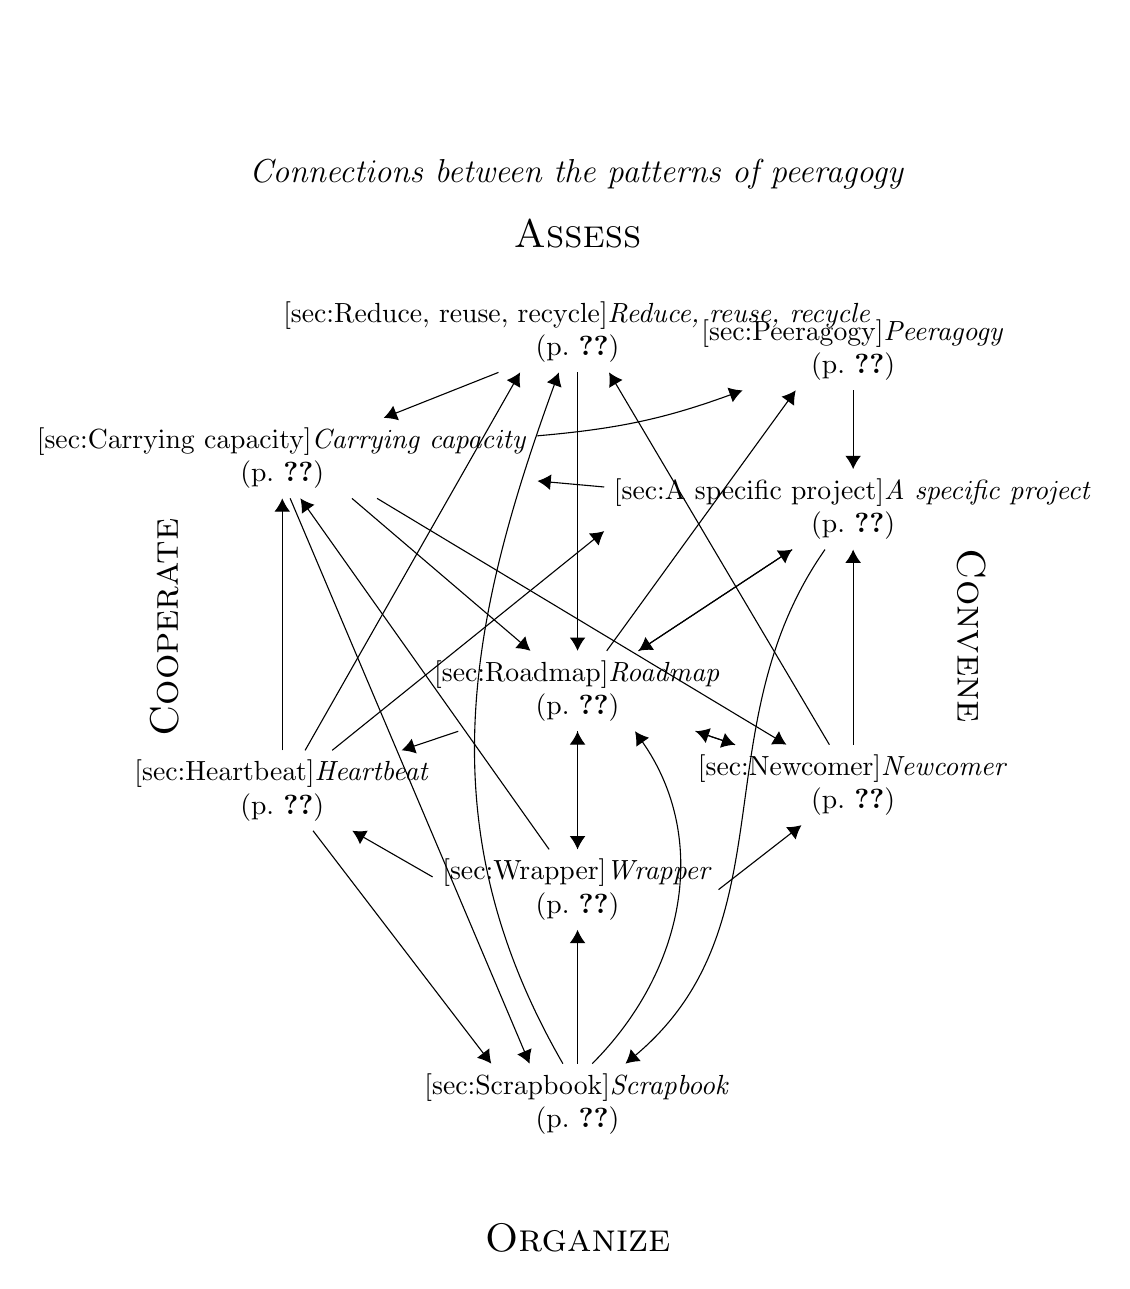
\begin{tikzpicture}[dot/.style={circle,inner sep=1pt,fill,name=#1},nodes = {align=center}]
\node (headline) at (5,10.75) {\large \emph{Connections between the patterns of peeragogy}};
%\draw[step=1cm,gray,very thin] (0,0) grid (10,10);
\node (assess) at (5, 10) {{\Large {\sc Assess}}};
\node (organize) at (5, -2.75) {{\Large {\sc Organize}}};
\node (cooperate)[text width=2cm,align=center,rotate=270] at (10, 5) {{\Large {\sc Convene}}};
\node (convene)[text width=15cm,align=center,rotate=90] at (-.25, 5) {{\Large {\sc Cooperate}}};
%%%%%%%%%%%%%%%%%%%%%%%%%%%%%%%%%%%%%%%%%%%%%%%%%%%%%%%%%%%%%%%%%%%%%%%%%%%%%%%%%%%%%%%%%%%%%%%%%%%%%
\node[below = 5cm of assess] (roadmap) {\hyperref[sec:Roadmap]{\emph{Roadmap}}\\(p.~\pageref{sec:Roadmap})};
\node (reduce) at (5, 8.75) {\hyperref[sec:Reduce, reuse, recycle]{\emph{Reduce, reuse, recycle}}\\(p.~\pageref{sec:Reduce, reuse, recycle})};
\node (carryingcapacity) at (1.25, 7.15) {\hyperref[sec:Carrying capacity]{\emph{Carrying capacity}}\\(p.~\pageref{sec:Carrying capacity})};
\node[below = 3.2cm of carryingcapacity] (heartbeat) {\hyperref[sec:Heartbeat]{\emph{Heartbeat}}\\(p.~\pageref{sec:Heartbeat})};
\node (aspecificproject) at (8.5, 6.5) {\hyperref[sec:A specific project]{\emph{A specific project}}\\(p.~\pageref{sec:A specific project})};
\node[below = 1.5cm of roadmap] (wrapper) {\hyperref[sec:Wrapper]{\emph{Wrapper}}\\(p.~\pageref{sec:Wrapper})};
\node (newcomer) at (8.5, 3) {\hyperref[sec:Newcomer]{\emph{Newcomer}}\\(p.~\pageref{sec:Newcomer})};
\node[below = 1.7cm of wrapper] (scrapbook) {\hyperref[sec:Scrapbook]{\emph{Scrapbook}}\\(p.~\pageref{sec:Scrapbook})};
\node[above = 1cm of aspecificproject] (peeragogyproject) {\hyperref[sec:Peeragogy]{\emph{Peeragogy}}\\(p.~\pageref{sec:Peeragogy})};
%%%%%%%%%%%%%%%%%%%%%%%%%%%%%%%%%%%%%%%%%%%%%%%%%%%%%%%%%%%%%%%%%%%%%%%%%%%%%%%%%%%%%%%%%%%%%%%%%%%%%
\draw[-{Latex[width=2mm]},draw=black] (peeragogyproject) -- (aspecificproject);
% \draw[-{Latex[width=2mm]},draw=black] (aspecificproject) -- (par);
\draw[-{Latex[width=2mm]},draw=black] (aspecificproject) -- (roadmap);
\draw[-{Latex[width=2mm]},draw=black] (aspecificproject.235) to[out=235,in=40] (scrapbook);
\draw[-{Latex[width=2mm]},draw=black] (aspecificproject) -- (carryingcapacity);
\draw[-{Latex[width=2mm]},draw=black] (carryingcapacity.337) -- (newcomer);
\draw[-{Latex[width=2mm]},draw=black] (carryingcapacity.330) -- (roadmap);
\draw[-{Latex[width=2mm]},draw=black] (carryingcapacity.5) to[out=5,in=200] (peeragogyproject);
\draw[-{Latex[width=2mm]},draw=black] ([xshift=1mm]carryingcapacity.south) -- (scrapbook.140);
% \draw[-{Latex[width=2mm]},draw=black] ([xshift=2mm]creatingaguide.160) to[out=-215,in=-67] (carryingcapacity);
\draw[-{Latex[width=2mm]},draw=black] (heartbeat) -- (aspecificproject.185);
\draw[-{Latex[width=2mm]},draw=black] (heartbeat) -- (carryingcapacity);
\draw[-{Latex[width=2mm]},draw=black] (heartbeat) -- (scrapbook.155);
\draw[-{Latex[width=2mm]},draw=black] (heartbeat) -- (reduce.215);
\draw[-{Latex[width=2mm]},draw=black] (newcomer) -- ([xshift=4mm]reduce.south);
\draw[-{Latex[width=2mm]},draw=black] (newcomer) -- (aspecificproject);
% \draw[-{Latex[width=2mm]},draw=black] (newcomer) -- (creatingaguide.north);
\draw[-{Latex[width=2mm]},draw=black] (newcomer) -- (roadmap);
% \draw[-{Latex[width=2mm]},draw=black] (par) -- (scrapbook);
\draw[-{Latex[width=2mm]},draw=black] (roadmap) -- (peeragogyproject.215);
\draw[-{Latex[width=2mm]},draw=black] (roadmap) -- (newcomer);
\draw[-{Latex[width=2mm]},draw=black] (roadmap) -- (wrapper);
\draw[-{Latex[width=2mm]},draw=black] (roadmap) -- (heartbeat);
\draw[-{Latex[width=2mm]},draw=black] (roadmap) -- (aspecificproject);
% \draw[-{Latex[width=2mm]},draw=black] (scrapbook) -- (par);
\draw[-{Latex[width=2mm]},draw=black] (scrapbook) -- (wrapper);
\draw[-{Latex[width=2mm]},draw=black] (scrapbook.110) to[out=120,in=250] (reduce.245);
\draw[-{Latex[width=2mm]},draw=black] (scrapbook.70) to[out=45,in=305] (roadmap.325);
% \draw[-{Latex[width=2mm]},draw=black] ([xshift=2mm,yshift=-.4mm]reduce.south) -- (creatingaguide);
\draw[-{Latex[width=2mm]},draw=black] ([xshift=4mm]reduce.200) -- (carryingcapacity);
\draw[-{Latex[width=2mm]},draw=black] (reduce) -- (roadmap);
\draw[-{Latex[width=2mm]},draw=black] (wrapper.175) -- (heartbeat);
\draw[-{Latex[width=2mm]},draw=black] ([xshift=-.5mm]wrapper.360) -- (newcomer);
\draw[-{Latex[width=2mm]},draw=black] (wrapper) -- ([xshift=2.3mm]carryingcapacity.south);
\draw[-{Latex[width=2mm]},draw=black] (wrapper) -- (roadmap);
\end{tikzpicture}


\par
}
\caption{Connections between the patterns of peeragogy.  An arrow points from pattern \textbf{A} to pattern \textbf{B} if the description of pattern \textbf{A} references pattern \textbf{B}. Labels at the borders of the figure correspond to the main sections of the \emph{Peeragogy Handbook}.\label{fig:connections}}
\end{figure}

% deferring a more detailed elaboration of next steps in the educational arena to future work that will build on this basis.
% Technology has come a long way since Alexander suggested ``you will get the most `power' over the language, and make it your own most effectively, if you write the changes in, at the appropriate places in the book'' \cite[p.~xl]{alexander1977pattern}.
% While Christian Kohls insightfully describes patterns as the unique resolution of the dynamical forces acting in a given context \cite{kohls2010structure,kohls2011structure}.
%%% Patterns come to you through mindful awareness ... Charlotte: I think about patterns all the time now, I think about what makes me productive in a team.
% So, while we speak the same language as other developers of design patterns, our orientation is somewhat different, and our understanding of the word `pattern' is nuanced because we aim to take full account of the lifecycle of patterns.  Our work contributes to a recent ``performative'' turn \cite{schummer2014beyond}, which we believe gets at the heart of what design patterns can do.
%  
% In practical terms, we believe the patterns that we introduce here will be useful for students and educators who want their work to have real-world relevance, to activists and policy-makers who want to develop practicable solutions to large-scale problems, and to employees and managers who, like it or not, find themselves working in distributed teams. 

\printbibliography[heading=subbibliography]
\end{refsection}
 \label{sec:Introduction}
%
\section{Peeragogy} \label{sec:Peeragogy}
\hypertarget{peeragogy}{%
\subsection{Peeragogy}\label{peeragogy}}

\hypertarget{motivation}{%
\subsubsection{Motivation}\label{motivation}}

This pattern is relevant to anyone who wants to do active learning
together with others in a relatively non-hierarchical setting.

\hypertarget{context}{%
\subsubsection{Context}\label{context}}

Collaborative projects like Wikipedia, StackExchange, and FLOSS
represent an implicit challenge to the old ``industrial'' organization
of work. This new way of working appears to promise something more
resilient, more exciting, and more humane. The rhetoric has been
questioned {{[}3,9{]}}. In and across these ``free'', ``open'',
post-modern organizations, individual participants are learning
{{[}7{]}} -- and that they collectively change the methods and
infrastructure as they go. Because everyone in these projects primarily
learns by putting in effort on a shared work-in-progress, participants
are more in touch with an \emph{equality of intelligence} than an
\emph{inequality of knowledge} {{[}4:38, 119{]}}. At the same time, they
invoke a form of friendly competition, in which \emph{the best
craftmanship wins} {{[}5:89{]}}.

\hypertarget{forces}{%
\subsubsection{Forces}\label{forces}}

\begin{quote}
\includegraphics{images/threshold.png} \textbf{Threshold}: inclusiveness
and specificity are in tension.\\
\includegraphics{images/trust.png} \textbf{Trust}: is only built through
sharing and reciprocity.
\end{quote}

\hypertarget{problem}{%
\subsubsection{Problem}\label{problem}}

Even a highly successful project like Wikipedia is a work in progress
that can be improved to \emph{better} empower and engage people around
the world, to develop \emph{richer and more useful} educational content,
and to disseminate it \emph{more} effectively -- and deploy it more
creatively.\footnote{\url{https://wikimediafoundation.org/wiki/Mission_statement}}
How to go about this is a difficult question, and we don't know the
answers in advance. There are rigorous challenges facing smaller
projects as well, and fewer resources to draw on. Many successful free
software projects are not particularly collaborative -- and the largest
projects are edited only by a small minority of users {{[}2,10{]}}. Can
we work smarter together?

\hypertarget{solution}{%
\subsubsection{Solution}\label{solution}}

The act of asking ``can we work smarter together?'' puts learning front
and center. Peeragogy takes that ``center'' and distributes it across a
pool of heterogeneous relationships. Indeed, peeragogy can be understood
as an up-to-date revision of Alexander's {{Network of Learning}}
{{[}1:99{]}}. It \emph{decentralizes the process of learning and
enriches it through contact with many places and people} in
interconnected networks that may reach all over the world. Importantly,
while people involved in a peeragogical process may be collaborating on
{{A specific project}}, they don't have to be direct collaborators
outside of the learning context or co-located in time or space. Just as
theories and practices of pedagogy articulate the transmission of
knowledge from teachers to students, peeragogy articulates the way peers
produce and use knowledge together (Figure {[}fig:connections{]}).

\hypertarget{rationale}{%
\subsubsection{Rationale}\label{rationale}}

The peeragogical approach particularly addresses the problems of small
projects stuck in their individual silos, and large projects becoming
overwhelmed by their own complexity. It does this by going the opposite
route: explicating \emph{what by definition is tacit} and employing
\emph{a continuous design process} {{[}8:9--10{]}}. As Howard Rheingold
remarks in the foreword to the \emph{Peeragogy Handbook}: ``What made
this work? Polycentric leadership is one key'' {{[}6:iii{]}}.
``Peer-led'' shouldn't suggest that there are no leaders: rather, it
means that multiple leaders act as peers.

\hypertarget{resolution}{%
\subsubsection{Resolution}\label{resolution}}

Peeragogy helps people in different projects describe and solve real
problems. If you share the problems that you're experiencing with
others, there's a reasonable chance that someone may be able to help you
solve them. Bringing a problem across the \textbf{threshold} of someone
else's awareness helps achieve clarity. This process can guide
individual action in ways that we wouldn't have seen on our own, and may
lead to new forms of collective action we would never have imagined
possible. People who gain experience comprehending problems together
build \textbf{trust}. Making room for multiple right answers contributes
further to resolving the tension between generality and specificity.

\hypertarget{example-1}{%
\subsubsection{Example 1}\label{example-1}}

Wikipedia and its sister sites Wiktionary, Wikiversity, etc.
(collectively ``Wikimedia'') rely on user-generated content, peer
produced software, and are managed, by and large, by a pool of users who
choose to get involved with governance and other ``meta''
duties.\footnote{\url{https://www.wikimedia.org/}} The Wikimedia
Foundation maintains the servers and acts on behalf of this ``global
movement''. They achieve something quite impressive: Wikipedia is the
7th most popular website in the world, but the Wikimedia Foundation has
under 300 employees. For comparison, the 6th (Amazon) and 8th (QQ) most
popular websites are run by companies with over 200K and 28K employees,
respectively.\footnote{\url{https://en.wikipedia.org/wiki/Wikimedia_Foundation\#Employees}},\footnote{\url{http://phx.corporate-ir.net/phoenix.zhtml?c=97664\&p=irol-newsArticle\&ID=2100418}},\footnote{\url{https://www.google.com/finance?cid=695431}},\footnote{\url{http://www.alexa.com/topsites}}

\includegraphics{images/Space_Surveillance_Telescope.jpg}
\emph{Observatory : Space Surveillance Telescope, New Mexico.}

\hypertarget{example-2}{%
\subsubsection{Example 2}\label{example-2}}

Although one of the strengths of {{Peeragogy}} is to distribute the
workload, this does not mean that infrastructure is irrelevant. The
students and researchers of the future university will need access to an
Observatory and other scientific apparatus if they are to reach \emph{ad
astra, per aspera} (Figure 1).\footnote{Latin: ``With difficulty, to the
  stars.''}

\hypertarget{whats-next-in-the-peeragogy-project}{%
\subsubsection{What's Next in the Peeragogy
Project*}\label{whats-next-in-the-peeragogy-project}}

We intend to revise and extend the \emph{Patterns of Peeragogy} into a
framework that can describe and scaffold the learning that happens
inside and outside of institutions.

\hypertarget{references}{%
\subsubsection{References}\label{references}}

\begin{enumerate}
\def\labelenumi{\arabic{enumi}.}
\item
  Christopher Alexander, Sara Ishikawa, and Murray Silverstein. 1977.
  \emph{A Pattern Language: Towns, Buildings, Construction}. Oxford
  University Press, Oxford.
\item
  Benjamin Mako Hill. 2011. When Free Software Isn't (Practically)
  Better. Retrieved from
  \url{http://www.gnu.org/philosophy/when_free_software_isnt_practically_better.html}
\item
  Daniel Kreiss, Megan Finn, and Fred Turner. 2011. The limits of peer
  production: Some reminders from Max Weber for the network society.
  \emph{New Media \& Society} 13, 2: 243--259.
\item
  Jacques Rancière. {[}1987{]} 1991. \emph{The ignorant schoolmaster:
  Five lessons in intellectual emancipation}. Stanford University Press.
\item
  Eric S Raymond. 2001. \emph{The Cathedral \& the Bazaar: Musings on
  Linux and open source by an accidental revolutionary}. O'Reilly Media,
  Inc.
\item
  H. Rheingold and others. 2015. \emph{The Peeragogy Handbook}.
  PubDomEd/Pierce Press, Chicago, IL./Somerville, MA. Retrieved from
  \url{http://peeragogy.org}
\item
  J. P. Schmidt. 2009. Commons-Based Peer Production and education.
  \emph{Free Culture Research Workshop, Harvard University}: 1--3.
  Retrieved from
  \url{http://cyber.law.harvard.edu/fcrw/sites/fcrw/images/Schmidt_Education_FreeCulture_25Oct2009.pdf}
\item
  Till Schümmer, Joerg M Haake, and Wolfgang Stark. 2014. Beyond
  rational design patterns. \emph{Proceedings of the 19th european
  conference on pattern languages of programs}, ACM, 13 pp.
\item
  Aaron Shaw and Benjamin Mako Hill. 2014. Laboratories of Oligarchy?:
  How the iron law extends to peer production. \emph{Journal of
  Communication} 64, 2: 215--238.
\item
  Aaron Swartz. 2006. Who Writes Wikipedia? Retrieved from
  \url{http://www.aaronsw.com/weblog/whowriteswikipedia}
\end{enumerate}

\begin{center}\rule{0.5\linewidth}{0.5pt}\end{center}

\hypertarget{notes}{%
\subsubsection{Notes}\label{notes}}

%
\section{Roadmap} \label{sec:Roadmap}
\hypertarget{roadmap}{%
\subsection{Roadmap}\label{roadmap}}

\hypertarget{motivation}{%
\subsection{Motivation}\label{motivation}}

This pattern shows how your group can define the scope of their project
and make a realistic plan to address it. This pattern provides the
backbone of our pattern language. It can be used to find a shared goal.

\hypertarget{context}{%
\subsection{Context}\label{context}}

\href{http://peeragogy.github.io/pattern-peeragogy.html}{Peeragogy} has
both distributed and centralized aspects. The discussants or
contributors who collaborate on a project have different points of view
and heterogeneous priorities, but they come together in conversations
and joint activities.

\hypertarget{forces}{%
\subsection{Forces}\label{forces}}

\begin{quote}
\Svariety\ \textbf{Variety}: people have different goals and interests in mind.\\
\Sclarity\ \textbf{Clarity}: some goals may be quite specific, and some rather vague.\\
\Scoherence\ \textbf{Coherence}: only some of these goals will be well-aligned.
\end{quote}

\hypertarget{problem}{%
\subsection{Problem}\label{problem}}

In order to collaborate, people need a way to share current, though
incomplete, understanding of the space they are working in, and to
nurture relationships with one another and the other elements of this
space. At the outset, there may not even be a coherent vision for a
project -- but a only loose collection of motivations and sentiments.
Once the project is up and running, people are likely to pull in
different directions.

\hypertarget{solution}{%
\subsection{Solution}\label{solution}}

Building a guide to the goals, activities, experiments and working
methods can help {{Newcomers}} and old-timers alike understand their
relationship with the project. It may combine features of a manifesto, a
syllabus, and an issue tracker. It may be a design pattern or a pattern
language {{[}3{]}}. The distinguishing qualities of a project Roadmap
are that it should be adaptive to circumstances, and that it should
ultimately get us from \emph{here} to \emph{there}. By this same token,
any given version of the roadmap is seen as fallible. In lieu of
widespread participation, the project's {{Wrapper}} should attempt to
synthesize an accurate roadmap that is informed by participants'
behavior, and should help moderate in case of conflict. Nevertheless,
full consensus is not necessary: different goals, with different
\emph{heres} and \emph{theres}, can be pursued separately, while
maintaining communication.

\hypertarget{rationale}{%
\subsection{Rationale}\label{rationale}}

The group evolves from a less-sophisticated to a more-sophisticated
manner of operating by using the roadmap. Using the roadmap builds a
collective awareness of how things are working in practice. In the
Peeragogy project our initial roadmap was a ``crowdsourced'' outline of
the first edition of the \emph{Peeragogy Handbook}. Later, it took the
form of a schedule of meetings following a regular {{Heartbeat}},
supplemented by a list of upcoming deadlines. Most recently, our roadmap
is expressed in the emergent objectives collected at the end of current
paper. We have seen that a list of nice-to-have features created in a
top-down fashion is comparatively unlikely to go anywhere! A backlog of
tasks and a realistic plan for accomplishing them are vastly different
things. An adaptive roadmap is an antidote to {{Tunnel Vision}}
{{[}1{]}}.

\hypertarget{resolution}{%
\subsection{Resolution}\label{resolution}}

An emergent roadmap is rooted in real problems and justifiable
solutions-in-progress in all their \textbf{variety} and communicates
both resolution and follow-through. The process of meshing varied issues
with one another requires thought and discussion, and this encourages
\textbf{clarity}. The test of \textbf{coherence} is that contributed
goals and ideas should be actionable. The ultimate quality-control test
is if it worked, i.e., did it come to pass that the task(s) the roadmap
was created to achieve ended up being achieved? If all of the issues
that the roadmap outlines are not resolved, the roadmap itself should be
revised. Without a roadmap, we would never know.

\hypertarget{example-1}{%
\subsection{Example 1}\label{example-1}}

The \emph{Help} link present on every Wikipedia page could be seen as a
localized {{Roadmap}} for individual user engagement: it tells users
what they can do with the site, and gives instructions on how to do
it.\footnote{\url{https://en.wikipedia.org/wiki/Help:Contents}} someone
who knows what they're doing, there are around 30 pages listing articles
with various kinds of problems, for example articles tagged with style
issues, or ``orphaned'' articles (i.e., articles with no links from
other pages in the encyclopedia).\footnote{\url{https://en.wikipedia.org/wiki/Category:Wikipedia_article_cleanup}},\footnote{\url{https://en.wikipedia.org/wiki/Category:Wikipedia_articles_with_style_issues}},\footnote{\url{https://en.wikipedia.org/wiki/Category:All_orphaned_articles}}
In 2010-2011, Wikimedia developed a strategic plan drawing on community
input {{[}2{]}}. In 2015, a two-week Community Consultation was carried
out; synthesis resulted in ``a direction that will guide the decisions
for the organization.''\footnote{\url{https://blog.wikimedia.org/2015/02/23/strategy-consultation/}}
Community-organized WikiProjects often invite and guide involvement on
{{A specific project}}.

\hypertarget{example-2}{%
\subsection{Example 2}\label{example-2}}

In a future university run in a peer produced manner, a fancy
President's Residence presumably wouldn't be needed. Leadership would be
carried out in a more collaborative and distributed fashion. However,
depending on just how distributed things are, it may turn out to be
useful for project facilitators to gather at a University Hall. Whereas
there is strength in numbers, there is leverage in organization. This is
what the {{Roadmap}} provides.

\includegraphics{images/alabama-small.jpg}\\
\emph{President's Residence, University of Alabama.}

\hypertarget{whats-next-in-the-peeragogy-project}{%
\subsection{What's Next in the Peeragogy
Project}\label{whats-next-in-the-peeragogy-project}}

If it becomes clear that something needs to change about the project,
that is a clue that we might need to revise our patterns or record a new
one. We can use the names of the patterns to tag our upcoming tasks.

\hypertarget{references}{%
\subsection{References}\label{references}}

\begin{enumerate}
\def\labelenumi{\arabic{enumi}.}
\item
  David M. Dikel, David Kane, and James R. Wilson. 2001. \emph{Software
  architecture: Organizational principles and patterns}. Pearson
  Education.
\item
  Eugene Eric Kim and others. 2011. \emph{Wikimedia Strategic Plan: A
  collaborative vision for the movement through 2015}. Wikimedia
  Foundation.
\item
  Christian Kohls. 2010. The structure of patterns. \emph{Proceedings of
  the 17th Conference on Pattern Languages of Programs}, ACM, 12.
\end{enumerate}

\begin{center}\rule{0.5\linewidth}{0.5pt}\end{center}

%
\section{Reduce, reuse, recycle} \label{sec:Reduce, reuse, recycle}
\hypertarget{reduce-reuse-recycle}{%
\subsection{Reduce, reuse, recycle}\label{reduce-reuse-recycle}}

\hypertarget{motivation}{%
\subsubsection{Motivation}\label{motivation}}

This pattern can guide project participants in identifying and managing
available resources.

\hypertarget{context}{%
\subsubsection{Context}\label{context}}

In a peer production context, you are simultaneously ``making stuff''
and building on the work of others.

\hypertarget{forces}{%
\subsubsection{Forces}\label{forces}}

\begin{quote}
\includegraphics{images/derivative.png} \textbf{Derivative}: you don't
have to do everything yourself!\\
\includegraphics{images/sensemaking.png} \textbf{Sensemaking}: resources
are useful only when you can make sense of them.\\
\includegraphics{images/sharing.png} \textbf{Sharing}: your
understanding gains robustness when you share with others.
\end{quote}

\hypertarget{problem}{%
\subsubsection{Problem}\label{problem}}

Many projects die because the cost of
{{\href{http://c2.com/cgi/wiki?ReinventingTheWheel}{Reinventing the
Wheel}}} {[}c2{]} is too high. However, this is just one possible
symptom of overfocus on a few priorities. Concerns may also arise if the
project's output is not actually used by anyone.

\hypertarget{solution}{%
\subsubsection{Solution}\label{solution}}

``Steal like an artist,'' and make it possible for other people to build
on your work too. In the Peeragogy project, we have used off-the-shelf
and hosted software suited to the task at hand (including: Drupal,
Google+, Google Hangouts, Google Docs, Wordpress, pandoc, Github,
ShareLaTeX). Early on we agreed to release our \emph{Peeragogy Handbook}
under the terms of the Creative Commons Public Domain Dedication (CC0),
the legal instrument that grants the greatest possible leeway to
downstream users.\footnote{\url{https://creativecommons.org/publicdomain/zero/1.0/}}
This has allowed us and others to repurpose and improve its contents in
other settings, including the current paper. Follow the steps indicated
by the keywords in the pattern's title:

\begin{itemize}
\tightlist
\item
  \emph{Reduce} the panoply of interesting interrelated ideas and
  methods to a functional core (e.g.~writing a book).
\item
  \emph{Reuse} resources relevant to this aim, factoring in ``things I
  was going to have to do anyway'' from everyone involved.
\item
  \emph{Recycle} what you've created in new connections and
  relationships.
\end{itemize}

\includegraphics{images/Duchamp_Fountaine.jpg}\\
\emph{A paradigmatic example of found-art. ``Fountain by R. Mutt,
Photograph by Alfred Stieglitz, THE EXHIBIT REFUSED BY THE
INDEPENDENTS''.}

\hypertarget{rationale}{%
\subsubsection{Rationale}\label{rationale}}

Clearly we are not the first people to notice the problems with
wheel-reinvention, including ``missing opportunities, repeating common
mistakes, and working harder than we need to.''\footnote{\url{https://blog.wikimedia.org/2013/11/19/learning-patterns-new-way-share-important-lessons/}}
As a guest in one of our hangouts, Willow Brugh, of Geeks without Bounds
and the MIT Media Lab, remarked that \emph{people often think that they
need to build a community, and so fail to recognize that they are
already part of a community.}\footnote{\url{https://www.youtube.com/watch?v=NpyQfYVKfBI}}
converted our old pattern catalog from the \emph{Peeragogy Handbook}
into this paper, sharing it with a new community and gaining new
perspectives; could we do something similar again?

\hypertarget{resolution}{%
\subsubsection{Resolution}\label{resolution}}

Reweaving old material into \textbf{derivative} designs and new material
into existing frameworks, we build deeper understanding, and carry out
collective \textbf{sensemaking}. The project's {{Roadmap}} develops by
making sense of existing resources -- including our worries and
concerns. Often we only know what these are when we attempt to
\textbf{share} them. Drawing on a wide range of resources boosts our
collective {{Carrying capacity}}.

\hypertarget{example-1}{%
\subsubsection{Example 1}\label{example-1}}

Contributors are encouraged to recycle existing works that are
compatible with the Wikimedia-wide Creative Commons
Attribution-ShareAlike (CC-By-SA) license.\footnote{\url{https://creativecommons.org/weblog/entry/15411/}}
Some sub-projects have been created purely to help repurpose other
existing works in this way.\footnote{\url{https://en.wikipedia.org/wiki/Wikipedia:WikiProject_Mathematics/PlanetMath_Exchange}}
On the downstream side, DBPedia is an important resource for the
semantic web, built by collating data from Wikipedia's
``infoboxes.''\footnote{\url{http://wiki.dbpedia.org/}} themselves
increasingly being populated automatically using information from
WikiData.\footnote{\url{https://www.wikidata.org/wiki/Wikidata:Main_Page}}
able to develop tools that reuse Wikipedia content in other ways
{{[}1,2{]}}, However, these research projects do not always result in a
tool that is accessible to day-to-day users.

\hypertarget{example-2}{%
\subsubsection{Example 2}\label{example-2}}

The knowledge resources and collaboration tools currently available
online are what make a low-cost, high-quality, formally-accredited
future university conceivable. However, the available resources are not
always as organized as they would need to be for educative purposes, so
peeragogues can usefully put effort into {{Reduce, reuse, recycle}}'ing
available resources into a functioning university Library.

\hypertarget{whats-next-in-the-peeragogy-project}{%
\subsubsection{What's Next in the Peeragogy
Project}\label{whats-next-in-the-peeragogy-project}}

Are there other educational resources and peeragogical case studies that
we could fold into our work? Can we recycle material from the
\emph{Peeragogy Handbook} into a format that is easier to understand and
apply?

\hypertarget{references}{%
\subsubsection{References}\label{references}}

\begin{enumerate}
\def\labelenumi{\arabic{enumi}.}
\item
  Silvan Reinhold. 2006. WikiTrails: Augmenting wiki structure for
  collaborative, interdisciplinary learning. \emph{Proceedings of the
  2006 International Symposium on Wikis}, ACM, 47--58.
\item
  Nathalie Henry Riche, Bongshin Lee, and Fanny Chevalier. 2010. IChase:
  Supporting exploration and awareness of editing activities on
  Wikipedia. \emph{Proceedings of the International Conference on
  Advanced Visual Interfaces}, ACM, 59--66.
\end{enumerate}

\begin{center}\rule{0.5\linewidth}{0.5pt}\end{center}
 
%
\section{Carrying Capacity} \label{sec:Carrying capacity}
\hypertarget{carrying-capacity}{%
\subsection{Carrying capacity}\label{carrying-capacity}}

\hypertarget{motivation}{%
\subsection{Motivation}\label{motivation}}

This pattern can help project participants recognize and communicate
their stresses to make themselves and the project more resilient.

\hypertarget{context}{%
\subsection{Context}\label{context}}

One of the important maxims from the world of FLOSS is: ``Given enough
eyeballs, all bugs are shallow'' {{[}8{]}}. A partial converse is also
true: there's only so much any one person can do, since we all have
limited time and energy.

\hypertarget{forces}{%
\subsection{Forces}\label{forces}}

\begin{quote}
\Santifragility\ \textbf{Antifragility}: each person's potential can only be realized if people take on enough, but not too much.\\
\Sindependence\ \textbf{Independence}: in a peeragogy context, it is often impossible to delegate work to others.
\end{quote}

\hypertarget{problem}{%
\subsection{Problem}\label{problem}}

How can we help prevent those people who are involved with the project
from over-promising or over-committing, and subsequently crashing and
burning? First, let's be clear that there are lots of ways things can go
wrong. Simplistic expectations -- like \emph{assuming that others will
do the work for you} {{[}13{]}} -- can undermine your ability to
correctly gauge your own strengths, weaknesses, and commitments. Without
careful, critical engagement, you might not even notice when there's a
problem. Where one person has trouble letting go, others may have
trouble speaking up. Pressure builds when communication isn't going
well.

\hypertarget{solution}{%
\subsection{Solution}\label{solution}}

Serious frustration is a sign that it's time to revisit the group's and
your own individual plan. Are these realistic? If you have a ``buddy''
they can provide a reality check. Maybe things are not \emph{that hard}
after all -- and maybe they don't need to be done \emph{right now}.
Generalizing from this: the project can promote an open dialog by
creating opportunities for people to share their worries and generate an
emergent plan for addressing them {{[}10{]}}. Use the project to make
note of obstacles. For example, if you'd like to pass a baton, you'll
need someone there who can take it. Maybe you can't find that person
right away, but you can bring up the concern and get it onto the
project's . The situation is always changing, but if we continue to
create suitable checkpoints and benchmarks, then we can take steps to
take care of an issue that's getting bogged down.

\hypertarget{rationale}{%
\subsection{Rationale}\label{rationale}}

Think of the project as an ecosystem populated by acts of participation.
As we get to know more about ourselves and each other, we know what
sorts of things we can expect, and we are able to work together more
sustainably {{[}6{]}}. We moderate stress and improve collective
outcomes by taking concerns seriously.

\hypertarget{resolution}{%
\subsection{Resolution}\label{resolution}}

Guiding and rebalancing behavior in a social context can begin with
speaking up about a concern. When we acknowledge concerns, we must take
into account our own boundedness. We have find an opportunity to make
ourselves helpful, without impinging on others' \textbf{independence}.
This doesn't mean allowing all possible stresses to run rampant: we work
to stay within the realm of \textbf{antifragility}, where manageable
stress \emph{improves} the system rather than degrading it {{[}12{]}}.
As we share concerns and are met with care and practical support, our
actions begin to align better with expectations (often as a result of
forming more realistic expectations).

\hypertarget{example-1}{%
\subsection{Example 1}\label{example-1}}

Wikipedia aims to emphasize a neutral point of view, but its users are
not neutral.\footnote{\url{https://en.wikipedia.org/wiki/Wikipedia:Neutral_point_of_view}}
topics that matter to them.\footnote{\url{https://en.wikipedia.org/wiki/Wikipedia:Activist}}
and participation are not neutral in another less sanguine sense. More
information on Wikipedia deals with Europe than all of the locations
outside of Europe {{[}2{]}}. As we remarked in the pattern, most of the
actual work is contributed by a small percentage of users. The
technology limits the kinds of things that can be said {{[}2{]}}. The
total number of active editors has been falling since 2007.\footnote{\url{https://strategy.wikimedia.org/wiki/Editor_Trends_Study/Results}}
Some blame outmoded technology and an insider culture {{[}11{]}}, or a
stringent editorial approach that emerged in response to the site's
popularity {{[}3{]}}. Others highlight the rise of successful
competition, often inspired by wiki models, but driven by ``corporate
logic'' {{[}4,5{]}}. Some proposed solutions focus on various indicators
of ``community health.''\footnote{\url{https://lists.wikimedia.org/pipermail/wiki-research-l/2016-January/004959.html}}

\hypertarget{example-2}{%
\subsection{Example 2}\label{example-2}}

Progressive thinkers have for some time subscribed to the view that
``there shall be no women in case there be not men, nor men in case
there be not women'' {{[}7{]}}. A separate Ladies Hall seems entirely
archaic. However, in light of the extreme gender imbalance in free
software, and still striking imbalance at Wikipedia {{[}1,9{]}}, it will
be important to do whatever it takes to make women and girls welcome,
not least because this is a significant factor in boosting our .

\includegraphics{images/ladies-hall.jpg}\\
\emph{Ladies Hall: Queens College, North Carolina.}

\hypertarget{whats-next-in-the-peeragogy-project}{%
\subsection{What's Next in the Peeragogy
Project}\label{whats-next-in-the-peeragogy-project}}

Making it easy and fruitful for others to get involved is one of the
best ways to redistribute the load. This often requires knowledge
transfer and skill development among those involved; see .

\hypertarget{references}{%
\subsection{References}\label{references}}

\begin{enumerate}
\def\labelenumi{\arabic{enumi}.}
\item
  Rishab A. Ghosh, Ruediger Glott, Bernhard Krieger, and Gregorio
  Robles. 2002. \emph{Free/Libre and Open Source Software: Survey and
  Study}. International Institute of Infonomics, University of
  Maastricht.
\item
  Mark Graham, Bernie Hogan, Ralph K Straumann, and Ahmed Medhat. 2014.
  Uneven geographies of user-generated information: Patterns of
  increasing informational poverty. \emph{Annals of the Association of
  American Geographers} 104, 4: 746--764.
\item
  Aaron Halfaker, R. Stuart Geiger, Jonathan Morgan, and John Riedl.
  2013. The Rise and Decline of an Open Collaboration System: How
  Wikipedia's reaction to sudden popularity is causing its decline.
  \emph{American Behavioral Scientist} 57, 5: 664--688.
  \url{http://doi.org/10.1177/0002764212469365}
\item
  Daniel Kreiss, Megan Finn, and Fred Turner. 2011. The limits of peer
  production: Some reminders from Max Weber for the network society.
  \emph{New Media \& Society} 13, 2: 243--259.
\item
  Mayo Fuster Morell. 2011. An introductory historical contextualization
  of online creation communities for the building of digital commons:
  The emergence of a free culture movement. \emph{Proceedings of the 6th
  Open Knowledge Conference}. Retrieved from
  \url{http://ceur-ws.org/Vol-739/paper_7.pdf}
\item
  Elinor Ostrom. 2010. Revising theory in light of experimental
  findings. \emph{Journal of Economic Behavior \& Organization} 73, 1:
  68--72.
\item
  François Rabelais. {[}1534{]} 1894. \emph{Gargantua and pantagruel}.
  Moray Press.
\item
  Eric S Raymond. 2001. \emph{The Cathedral \& the Bazaar: Musings on
  Linux and open source by an accidental revolutionary}. O'Reilly Media,
  Inc.
\item
  Joseph Reagle. 2012. ``Free as in sexist?'' Free culture and the
  gender gap. \emph{First Monday} 18, 1. Retrieved from
  \url{http://firstmonday.org/ojs/index.php/fm/article/view/4291}
\item
  Jaakko Seikkula and Tom Erik Arnkil. 2006. \emph{Dialogical meetings
  in social networks}. Karnac Books.
\item
  Tom Simonite. 2013. The Decline of Wikipedia. \emph{Technology Review}
  116, 6: 50--56.
\item
  Nassim Nicholas Taleb. 2012. \emph{Antifragile: Things that gain from
  disorder}. Random House Incorporated.
\item
  Linus Torvalds and Steven Vaughan-Nichols. 2011. Linus Torvalds's
  Lessons on Software Development Management. \emph{Input Output}.
  Retrieved from
  \url{http://web.archive.org/web/20131021211847/http://h30565.www3.hp.com/t5/Feature-Articles/Linus-Torvalds-s-Lessons-on-Software-Development-Management/ba-p/440}
\end{enumerate}

\begin{center}\rule{0.5\linewidth}{0.5pt}\end{center}

%
\section{A specific project} \label{sec:A specific project}
\hypertarget{a-specific-project}{%
\subsection{A specific project}\label{a-specific-project}}

\hypertarget{motivation}{%
\subsection{Motivation}\label{motivation}}

This pattern can help project participants get started, get focused, and
make concrete change. It is especially useful for someone who is
currently feeling stuck.

\hypertarget{context}{%
\subsection{Context}\label{context}}

We often find ourselves confronted with what seems to be a difficult,
complex, or even insurmountable problem. It won't go away, but a
workable solution doesn't present itself, either. If there is a
candidate solution, it's also clear there are not enough resources for
it to be feasible.

\hypertarget{forces}{%
\subsection{Forces}\label{forces}}

\begin{quote}
\Sdifficulty\ \textbf{Difficulty}: bringing about meaningful change is often hard work.\\
\Sinertia\ \textbf{Inertia}: when things are hard we may feel stuck, wring our hands, or preach to the choir.
\end{quote}

\hypertarget{problem}{%
\subsection{Problem}\label{problem}}

One is often blinded by one's prejudices and preferences. Some may put
considerable energy into pondering, discussing, exploring and feeling
stuck. Some may want more concrete progress, and notice the time passing
by. In a group setting, when the forward-movers ultimately try to act,
those who are more wrapped up in the experience of pondering and
exploring may rebel, if they feel that they are being left behind.
Inaction may seem like the only safe choice, but it has risks too. And,
once moving, things can easily get bogged down again.

\hypertarget{solution}{%
\subsection{Solution}\label{solution}}

One way to make progress when you're stuck is to ask a specific question
to someone who may be able to help you get unstuck. Formulating a
question helps your thinking become more concrete. Sometimes you'll see
that a solution was within your grasp all along. Often, one question
won't be enough, but you can repeat the process. In this way, you can
reduce a large, complex, or ephemeral concern into a collection of
smaller, specific, manageable tasks with clear next steps and success
criteria. Use a {{Scrapbook}} to make note of all the small things, and
weave them into your project {{Roadmap}}. This will show how the small
pieces relate to the bigger picture. If you have a fairly specific idea
about what you want to do, but you're finding it difficult to get it
done, don't just ask for advice: recruit material help (cf.~{{Carrying
capacity}}). One example of a specific project from the Peeragogy
project is our work on this paper, which had a specific target audience,
a set of associated deadlines, and allowed us to get help from pattern
experts.

\hypertarget{rationale}{%
\subsection{Rationale}\label{rationale}}

We've seen time and again that having a specific project is a recipe for
getting concrete, and that getting concrete is necessary for bringing
about change. Asking for help (which is what happens when you vocalize a
question) is one of the best ways to gain coherence. Making yourself
understood can go a long way toward resolving deeper difficulties.

\hypertarget{resolution}{%
\subsection{Resolution}\label{resolution}}

Where you run into \textbf{difficulty}, getting specific paves the way
for incremental forward progress and helps to overcome \textbf{inertia}.
The struggle between consensus and action is resolved in a tangible
project that combines action with dialog. Learning something new is a
strong sign that things are working. In the Peeragogy project, we have
completed many projects during our weekly hangouts, for example ``hive
editing'' an abstract for submission to a conference.

\hypertarget{example-1}{%
\subsection{Example 1}\label{example-1}}

At first glance, the Wikimedia Foundation's mission may seem like a good
idea, but hard to do anything about.\footnote{\url{https://wikimediafoundation.org/wiki/Mission_statement}}
practice, many Wikipedians contribute to the mission by working on {{A
specific project}}.

\includegraphics{images/Ruin_Academy_Dorm.jpg} \emph{Dormitory, Ruin
Academy, Taipei, Taiwan.}

Within Wikipedia, these are known as
``WikiProjects.''\footnote{\url{https://en.wikipedia.org/wiki/Wikipedia:WikiProject_Council/Directory}},\footnote{\^{}fn3}
on how to start new WikiProjects.\footnote{\url{https://en.wikipedia.org/wiki/Wikipedia:WikiProject_Council/Guide/WikiProject}}
Wikimedia Foundation also runs other public projects, including the
Wikipedia Education Program and the GLAM Wiki (for Galleries, Libraries,
Archives, and Museums).\footnote{\url{https://outreach.wikimedia.org/wiki/Education/Wikipedia_Education_Collaborative/Tasks}},\footnote{\url{https://outreach.wikimedia.org/wiki/GLAM}}
\emph{list of case studies that describes specific projects undertaken
by cultural organizations and Wikimedia}.\footnote{\url{https://outreach.wikimedia.org/wiki/GLAM/Case_studies}}

\hypertarget{example-2}{%
\subsection{Example 2}\label{example-2}}

Collegial and convivial peer support via remote collaboration or
short-term meet-ups may fill some of the requirements of ``student
life''. Peeragogy can also happen in neighborhoods, and among persons
sharing long-term co-habitation. While a traditional Dormitory may not
be necessary, a shared rented or cooperatively-owned living/working
environment could be an asset for peeragogues working together on {{A
specific project}}.

\hypertarget{whats-next-in-the-peeragogy-project}{%
\subsection{What's Next in the Peeragogy
Project}\label{whats-next-in-the-peeragogy-project}}

Let's use our pattern catalog to build specific, tangible ``what's
next'' steps, add them to our {{Roadmap}}, and carry them out with
concrete actions. Let's be sure we know who's responsible for what, and
employ a ``buddy system'' to help get things done.

\begin{center}\rule{0.5\linewidth}{0.5pt}\end{center}

%
\section{Wrapper} \label{sec:Wrapper}
\hypertarget{wrapper}{%
\subsection{Wrapper}\label{wrapper}}

\hypertarget{motivation}{%
\subsection{Motivation}\label{motivation}}

This pattern suggests to find at least one person to fill an important
role managing the project's public interface, and keeping participants
up to date about activities.

\hypertarget{context}{%
\subsection{Context}\label{context}}

You are part of an active, long-running, and possibly quite complex
project with more than a handful of participants. How do you manage?

\hypertarget{forces}{%
\subsection{Forces}\label{forces}}

\begin{quote}
\Sinterface\ \textbf{Interface}: the project shows people how they can use it.\\
\Sfamiliar\ \textbf{Familiarity}: the leader/follower dichotomy is easy to understand.\\
\Sequity\ \textbf{Equity}: peeragogy aims for fairness.
\end{quote}

\hypertarget{problem}{%
\subsection{Problem}\label{problem}}

In an active project, it can be effectively impossible to stay up to
date with all of the details. Not everyone will be able to attend every
meeting (see {{Heartbeat}}) or read every email. Project participants
can easily get lost and drift away. The experience can be much more
difficult for {{Newcomers}}: joining an existing project can feel like
trying to climb aboard a rapidly moving vehicle. Information overload is
not the only concern: there is also a problem with missing information.
If key skills are not shared, they can quickly become bottlenecks (see
{{Carrying capacity}}).

\includegraphics{images/dashboard_design.jpg} \emph{Design for a
Peeragogy project dashboard (sketch by Amanda Lyons, prototype by
Fabrizio Terzi).}

\hypertarget{solution}{%
\subsection{Solution}\label{solution}}

Someone involved with the project should regularly create a wrap-up
summary, distinct from other project communications, that makes current
activities comprehensible to people who may not have been following all
of the details. In addition, project members should keep other
informative resources like the landing page, {{Roadmap}}, and
documentation up to date. Check empirically to see if they really show
interested parties how they can get involved. Building on the idea of a
``project dashboard,'' we can guide potential contributors to live help;
we can then see what questions they ask.\footnote{\url{https://gitter.im/orgs/Peeragogy/rooms}}
{{Wrapper}} is both a role, and, sometimes, an artifact. Our
\emph{Handbook}'s cover literally wraps up its contents; the
collaboratively written chat notes from our weekly Hangouts give a
collaboratively-written overview of what was discussed in the meeting.
Meetings themselves can be structured to give people a chance to sum up
what they've accomplished during the week, as well as any problems they
are running into. Between meetings, each participant is advised to
maintain some sort of ``learning log'' in the form of a personal
{{Scrapbook}}, so that outstanding concerns are surfaced and available
to discuss.

\hypertarget{rationale}{%
\subsection{Rationale}\label{rationale}}

According to the theory proposed by Yochai Benkler, for free/open
``commons-based'' projects to work, it is important for participants to
be able to contribute small pieces, and for the project to have a way to
stitch those pieces together {{[}1{]}}. The {{Wrapper}} helps perform
this integrative stitching function. If you value participation, you may
have to do some serious work to facilitate access to process.

\hypertarget{resolution}{%
\subsection{Resolution}\label{resolution}}

Well-maintained records chronicle the project's history; up-to-date
documentation makes the project more robust; a coherent look-and-feel
offers an accessible \textbf{interface} to the outside world. Regularly
circulated summaries can help to engage or re-engage members of a
project, and can give an emotional boost to peeragogues who see their
contributions and concerns mentioned, giving less engaged participants
the \textbf{familiar} experience of ``following'' someone else's
updates. People will judge from experience whether the project strives
for \textbf{equity} or strives to maintain hidden power differentials.

\hypertarget{example-1}{%
\subsection{Example 1}\label{example-1}}

There are many data streams around the Wikimedia project. They comprise
an elaborate {{Wrapper}} function for the project, with components that
range from Today's Featured Article, which appears on the front page of
Wikipedia, to formal annual reports from the
nonprofit.\footnote{\url{https://en.wikipedia.org/wiki/Wikipedia:Today\%27s_featured_article}},\footnote{\url{https://wikimediafoundation.org/wiki/Annual_Report}}

\hypertarget{example-2}{%
\subsection{Example 2}\label{example-2}}

In-person meetings are just as relevant for contemporary humans as they
were a century ago, even though we have learned more about how to
assemble on the fly {{[}2{]}}. Getting together for conventions, dance
parties, and commencement ceremonies could comprise an important part of
the future university's {{Wrapper}} function, even if these events do
not always take place in one specific Assembly Hall.

\hypertarget{whats-next-in-the-peeragogy-project}{%
\subsection{What's Next in the Peeragogy
Project}\label{whats-next-in-the-peeragogy-project}}

Let's make sure we have protocols in place that enable us to share
progress, and to revise our ``next steps'' if people are getting stuck.
Let's improve the interaction design for peeragogy.org so that it's
clear how people can get involved.

\hypertarget{references}{%
\subsection{References}\label{references}}

\begin{enumerate}
\def\labelenumi{\arabic{enumi}.}
\item
  Y. Benkler. 2002. Coase's Penguin, or Linux and the Nature of the
  Firm. \emph{Yale Law Journal} 112: 369.
\item
  Howard Rheingold. 2007. \emph{Smart mobs: The next social revolution}.
  Basic books.
\end{enumerate}

\begin{center}\rule{0.5\linewidth}{0.5pt}\end{center}

%
\section{Heartbeat} \label{sec:Heartbeat}
\hypertarget{heartbeat}{%
\subsection{Heartbeat}\label{heartbeat}}

\hypertarget{motivation}{%
\subsubsection{Motivation}\label{motivation}}

This pattern can help project participants stay in touch, and stay
motivated.

\hypertarget{context}{%
\subsubsection{Context}\label{context}}

A number of people have a shared interest, and have connected with each
other about it. However, they are not going to spend 24 hours a day, 7
days a week working together, either because they are busy with other
things, or because working separately on some tasks is vastly more
efficient.

\hypertarget{forces}{%
\subsubsection{Forces}\label{forces}}

\begin{quote}
\includegraphics{images/differentiation.png} \textbf{Differentiation}:
the time we spend together isn't all equally meaningful.\\
\includegraphics{images/entropy.png} \textbf{Entropy}: something needs
to hold the project together, or it will fall apart.
\end{quote}

\hypertarget{problem}{%
\subsubsection{Problem}\label{problem}}

How will the effort be sustained and coordinated sufficiently? How do we
know this an active collaboration, and not just a bunch of people
milling about? Is there a \emph{there, there?}

\hypertarget{solution}{%
\subsubsection{Solution}\label{solution}}

People seem to naturally gravitate to something with a pulse. \emph{Once
a day} (stand-ups), \emph{once a week} (meetings), or \emph{once a year}
(conferences, festivals) are common variants. When the project is
populated by more than just a few people, it's likely that there will be
several {{Heartbeats}}, building a sophisticated polyrhythm. A
well-running project will feel ``like an improvisational jazz ensemble''
{{[}1{]}}. Much as the band director may gesture to specific players to
invite them to solo or sync up, a project facilitator may craft
individual emails to ask someone to lead an activity or invite them to
re-engage. Two common rhythm components are weekly synchronous meetings
with an open agenda, combined with \emph{ad hoc} meetings for focused
work on {{A specific project}}. The precise details will depend on the
degree of integration required by the group.

\hypertarget{rationale}{%
\subsubsection{Rationale}\label{rationale}}

The project's heartbeat is what sustains it. Just as \emph{people matter
more than code} {{[}2{]}}, so does the life of the working group matter
more than mechanics of the work structure. Indeed, there is an quick way
to do a reality check and find the project's strongest pulse: the
activities that sustain a healthy project should sustain us, too
(cf.~{{Carrying capacity}}).

\hypertarget{resolution}{%
\subsubsection{Resolution}\label{resolution}}

Noticing when a new {{Heartbeat}} is beginning to emerge is a way to be
aware of the shifting priorities in the group, and contributes to
further \textbf{differentiation}. This may ultimately be a good source
of new patterns. On the other hand, if a specific activity is no longer
sustaining the project, stop doing it, much as you would move an
out-of-date pattern to the {{Scrapbook}} in order to make room for other
concerns. The power of the {{Heartbeat}} is that the project can be as
focused and intensive as it needs to be, working against
\textbf{entropy} in the ways that start to be required as time goes by.

\hypertarget{example-1}{%
\subsubsection{Example 1}\label{example-1}}

The yearly in-person gathering, Wikimania, is the most visible example
of a {{Heartbeat}} for the Wikimedia movement.\footnote{\url{https://meta.wikimedia.org/wiki/Wikimania}}
may run additional in-person get-togethers.\footnote{\url{http://wikiconferenceusa.org/}}
Also of note is the twice-yearly call for proposals for individual
engagement grants.\footnote{\url{https://meta.wikimedia.org/wiki/Grants:IEG}}
other shorter cycles. Each day a highly-vetted Featured Article appears
on the front page of Wikipedia, and is circulated to a special-purpose
mailing list.\footnote{\url{https://en.wikipedia.org/wiki/Wikipedia:Today\%27s_featured_article}},\footnote{\url{https://en.wikipedia.org/wiki/Wikipedia:Featured_article_candidates}},\footnote{\url{https://lists.wikimedia.org/mailman/listinfo/daily-article-l}}
articles for deletion lasts at least seven days.\footnote{\url{https://en.wikipedia.org/wiki/Wikipedia:Articles_for_deletion}}

\includegraphics{images/kapisa.jpg}\\
\emph{University Farm: al-Biruni University, Kapisa province,
Afghanistan.}

\hypertarget{example-2}{%
\subsubsection{Example 2}\label{example-2}}

Although it may sound quaint, some variant of the University Farm could
help to physically sustain peeragogues, while putting the project's
{{Heartbeat}} in tune with that of the seasons. In the current
distributed mode, we tend our window boxes and allotment gardens. New
developments should unfold in a \emph{logical order growing out of the
needs of the community} {{[}3{]}}.

\hypertarget{whats-next-in-the-peeragogy-project}{%
\subsubsection{What's Next in the Peeragogy
Project}\label{whats-next-in-the-peeragogy-project}}

\begin{quote}
Actual meeting times to be added
\end{quote}

Identifying and fostering new {{Heartbeats}} and new working groups can
help make the community more robust. This is the time dimension of
spin-off projects described in {{Reduce, reuse, recycle}}.

\hypertarget{references}{%
\subsubsection{References}\label{references}}

\begin{enumerate}
\def\labelenumi{\arabic{enumi}.}
\item
  David M. Dikel, David Kane, and James R. Wilson. 2001. \emph{Software
  architecture: Organizational principles and patterns}. Pearson
  Education.
\item
  Linus Torvalds and Steven Vaughan-Nichols. 2011. Linus Torvalds's
  Lessons on Software Development Management. \emph{Input Output}.
  Retrieved from
  \url{http://web.archive.org/web/20131021211847/http://h30565.www3.hp.com/t5/Feature-Articles/Linus-Torvalds-s-Lessons-on-Software-Development-Management/ba-p/440}
\item
  Booker T Washington. 1901. \emph{Up from slavery}. Doubleday \&
  Company, Inc.
\end{enumerate}

\begin{center}\rule{0.5\linewidth}{0.5pt}\end{center}

%
\section{Newcomer} \label{sec:Newcomer}
\hypertarget{newcomer}{%
\subsection{Newcomer}\label{newcomer}}

\hypertarget{motivation}{%
\subsubsection{Motivation}\label{motivation}}

This pattern can help project participants be aware of the issues faced
by newcomers, and cultivate a ``beginner's mind'' themselves.

\hypertarget{context}{%
\subsubsection{Context}\label{context}}

When there's learning happening, it's because there is someone who is
new to a topic, or to something about the topic.

\hypertarget{forces}{%
\subsubsection{Forces}\label{forces}}

\begin{quote}
\includegraphics{images/individuation.png} \textbf{Individuation}: each
person learning optimally is what's best for the community.\\
\includegraphics{images/mutuality.png} \textbf{Mutuality}: our
individuality does not isolate us from one another, but draws us
together.
\end{quote}

\hypertarget{problem}{%
\subsubsection{Problem}\label{problem}}

Newcomers can feel overwhelmed by the amount of things to learn. They
often don't know where to start. They may have a bunch of ideas that the
old-timers have never considered -- or they may think they have new
ideas, which are actually a different take on an old idea; see {{Reduce,
reuse, recycle}}. People who are new to the project can tell you what
makes their participation difficult. Since you're learning as you go as
well, you can ask yourself the same question: what aspects of this
encounter are difficult for me?

\hypertarget{solution}{%
\subsubsection{Solution}\label{solution}}

Instead of thinking of newcomers as ``them'', and trying to provide
solutions, we focus on newcomers as ``us'' -- which makes the search for
solutions that much more urgent. We permit ourselves to ask naive
questions. We entertain vague ideas. We add concreteness by trying {{A
specific project}}. We may then genuinely turn to others for help. We
aim to foster a culture in which the focus for everyone is on addressing
our own learning challenges rather than on ``providing'' solutions for
others {{[}1{]}}. When you begin a new project, try to systematically
take notes and gather data to analyze and reflect upon later; leave
artifacts for other future newcomers to use and build upon in their own
research. In practice this may be a lot to ask for someone just joining
a group, but over time we may have many ways to structure our collective
engagement so that it leads to research cycles based on the ``action
research'' steps \emph{reflect}, \emph{plan}, \emph{act}, and
\emph{observe}. Note that there is a parallel with the four facets
\emph{assess}, \emph{convene}, \emph{organize}, \emph{cooperate} from
Figure {[}fig:connections{]}. The history of the action research
approach, with particular emphasis on educational applications, is
surveyed in {{[}5{]}}. One method for doing the reflection/assessment
step is presented in the {{Scrapbook}} pattern. Be flexible: networked
attention (even more so than rigid cycles {{[}3{]}}) leads to new ways
of knowing and expanded access to knowledge-production {{[}7,8{]}}.

\hypertarget{rationale}{%
\subsubsection{Rationale}\label{rationale}}

A newcomer's confusion about how best to get involved or what the point
of all this actually is may be due to a lack of structure in the project
{{Roadmap}}. Sharing vulnerability and confusion gives us a chance to
learn.

\hypertarget{resolution}{%
\subsubsection{Resolution}\label{resolution}}

An awareness of the difficulties that newcomers face can help us be more
compassionate to ourselves and others. We strengthen the community by
supporting all participants' \textbf{individuation}. We have a better
chance of making the project useful for others if we're clear about how
it is useful to \emph{us}. By welcoming newcomers, we enhance the sense
of \textbf{mutuality} with people who have never encountered the project
before, and learn together with them. The facts start to become useful
when we understand how people perceive them {{[}4{]}}.

\hypertarget{example-1}{%
\subsubsection{Example 1}\label{example-1}}

Wikipedia {{Newcomers}} can make use of resources that include a
``Teahouse'' where questions are welcomed, a platform extension that
changes the user interface for new editors, and lots of
documentation.\footnote{\url{https://en.wikipedia.org/wiki/Wikipedia:Teahouse}},\footnote{\url{https://en.wikipedia.org/wiki/Wikipedia:GettingStarted}},\footnote{\url{https://en.wikipedia.org/wiki/Help:Editing}}
exceptional newcomers may be given special recognition.\footnote{\url{https://en.wikipedia.org/wiki/Template:The_New_Editor\%27s_Barnstar}}
interest to the Wikimedia Foundation.\footnote{\url{https://meta.wikimedia.org/wiki/Research:Newcomer_survival_models}}
However, ``Nearly all editors begin with a burst of activity, then
quickly tail off'' {{[}6{]}}. The degree to which those editors who are
retained strive to maintain a ``beginner's mind'' is less clear. As
regards learning their way around the community, there is quantitative
support {{[}6{]}} for the claim that ``novice users learn the rules and
conventions for contributing both through observation and direct
coaching from more knowledgeable others'' {{[}2{]}}.

\includegraphics{images/The_Science_Laboratory.jpg}\\
\emph{Science Hall: Aspatria Agricultural College, Aspatria, Cumberland,
UK}

\hypertarget{example-2}{%
\subsubsection{Example 2}\label{example-2}}

It will often be pragmatic to connect {{Newcomers}} with employment
directly, so that the future university may see a closer coupling of
science and industry than would be found in the old Science Hall.
Inspiration can be drawn the London-based freelancing cooperative
Founders\&Coders, which is able to offer intensive training in web
development at no cost to successful applicants, on the basis that some
trainees will choose to join the cooperative as paying members later
on.\footnote{\url{http://www.foundersandcoders.com/academy/}}

\hypertarget{whats-next-in-the-peeragogy-project}{%
\subsubsection{What's Next in the Peeragogy
Project}\label{whats-next-in-the-peeragogy-project}}

More detailed guides can show {{Newcomers}} how they can contribute and
what to expect when they do. We should have different guides for
different ``user stories''. We can start by listing some of the things
we're currently learning about.

\hypertarget{references}{%
\subsubsection{References}\label{references}}

\begin{enumerate}
\def\labelenumi{\arabic{enumi}.}
\item
  D. Boud and A. Lee. 2005. ``Peer learning'' as pedagogic discourse for
  research education. \emph{Studies in Higher Education} 30, 5:
  501--516.
\item
  Susan L Bryant, Andrea Forte, and Amy Bruckman. 2005. Becoming
  Wikipedian: Transformation of participation in a collaborative online
  encyclopedia. \emph{Proceedings of the 2005 international aCM sIGGROUP
  conference on supporting group work}, ACM, 1--10.
\item
  Y. Engeström. 1999. Innovative learning in work teams: Analyzing
  cycles of knowledge creation in practice. In \emph{Perspectives on
  activity theory}, Yrjö Engeström, Reijo Miettinen and Raija-Leena
  Punamäki (eds.). Cambridge University Press, 377--406.
\item
  Paulo Freire. 1982. Creating alternative research methods: Learning to
  do it by doing it. In \emph{Creating knowledge: A monopoly}, B. Hall,
  A. Gillette and R. Tandon (eds.). Society for Participatory Research
  in Asia, 29--37.
\item
  Jean McNiff. 2013. \emph{Action research: Principles and practice}.
  Routledge.
\item
  Katherine Panciera, Aaron Halfaker, and Loren Terveen. 2009.
  Wikipedians are born, not made: A study of power editors on Wikipedia.
  \emph{Proceedings of the aCM 2009 international conference on
  supporting group work}, ACM, 51--60.
\item
  Gilbert Simondon. 2012. Technical mentality. In \emph{Gilbert
  Simondon: Being and technology}, Arne De Boever, Alex Murray, Jon
  Roffe and Ashley Woodward (eds.). Oxford University Press, 1--15.
\item
  C.S. Wagner. 2008. \emph{The new invisible college: Science for
  development}. Brookings Inst Press.
\end{enumerate}

\begin{center}\rule{0.5\linewidth}{0.5pt}\end{center}

%
\section{Scrapbook} \label{sec:Scrapbook}
\hypertarget{scrapbook}{%
\subsection{Scrapbook}\label{scrapbook}}

\hypertarget{motivation}{%
\subsection{Motivation}\label{motivation}}

This pattern describes a way to make the project meaningful.

\hypertarget{context}{%
\subsection{Context}\label{context}}

We have been working together for a while now. We have maintained and
revised our pattern catalog, and we are achieving some of the ``What's
Next'' steps associated with some of the patterns.

\hypertarget{forces}{%
\subsection{Forces}\label{forces}}

\begin{quote}
\Sattention\ \textbf{Attention}: due to limited energy, we need to ask: where should we set the focus?
\Sinterest\ \textbf{Interest}: new experiences catch our attention.
\Smeaning\ \textbf{Meaning}: shared history makes things meaningful.
\end{quote}

\hypertarget{problem}{%
\subsection{Problem}\label{problem}}

Not all of the ideas we've come up with have proved workable. Not all of
the patterns we've noticed remain equally relevant. In particular, some
patterns no longer lead to concrete next steps.

\hypertarget{solution}{%
\subsection{Solution}\label{solution}}

In order to maintain focus, is important to ``tune'' and ``prune'' the
things we give our attention to. We can connect this understanding to
any actions undertaken in the project by asking questions like these:

\begin{quote}
(1) Review what was supposed to happen. (2) Establish what is
happening/happened. (3) Determine what's right and wrong with what we
are doing/have done. (4) What did we learn or change? (5) What else
should we change going forward? {{[}9{]}}, after {{[}10{]}}.
\end{quote}

Other review processes have been formalized, including the design review
in architecture and the postmortem in theater and other teamwork
settings {{[}7,8{]}}. The review process may benefit from having an
experienced facilitator on board {{[}6{]}}. As current priorities become
clearer, we decide where to focus. Anything that isn't receiving active
attention should be moved to a {{Scrapbook}}. This may encompass:

\begin{itemize}
\tightlist
\item
  \emph{Retired patterns} that are tabled or completed (no more next
  steps);
\item
  \emph{Proto-patterns} made of problems, issues, and concerns;
\item
  \emph{A back-catalog} of publications, reports, or other artifacts.
\end{itemize}

In the Peeragogy project, alongside our patterns we initially maintained
a collection of antipatterns (like `{{Magical thinking}}') but the next
steps coming from these seemed particularly convoluted and abstract. So,
we archived them.\footnote{\url{http://paragogy.net/Scrapbook}} problems
-- without known solutions -- right up front in the Introduction to the
\emph{Peeragogy Handbook} {{[}9{]}}. Other proto-patterns include
`{{Onboarding}}' and `{{Don't quit your day job}}', which arose in our
review of this paper (see ``Emergent Roadmap'', below). Our back-catalog
includes academic papers {{[}14{]}} and a thesis {{[}5{]}}. Everyone can
maintain their own personal {{Scrapbook}} as along with a communal one.
Furthermore, you don't need to limit yourself to \emph{your own}
creativity: include interesting ideas from other sources (see {{Reduce,
reuse, recycle}}). In some cases a designated {{Wrapper}} may have to do
further work to elicit and organize contributions.

\hypertarget{rationale}{%
\subsection{Rationale}\label{rationale}}

We want to keep attention focused on the most relevant issues. If a
pattern, task, or concern does not lead to concrete ``next steps'' at
the moment, sufficient time for reflection may offer a better
understanding, and it may prove useful and actionable in a different
context.

\hypertarget{resolution}{%
\subsection{Resolution}\label{resolution}}

Judicious use of the {{Scrapbook}} can help focus project participants'
\textbf{attention} on current concerns, without losing grasp of items of
\textbf{interest}. The currently active pattern catalog is leaner and
more action-oriented as a result. If the {{Roadmap}} shows where we're
going, it is the {{Scrapbook}} that shows most clearly where we've been,
and collects the observations that are most \textbf{meaningful} to us.

\hypertarget{example-1}{%
\subsection{Example 1}\label{example-1}}

The history of the Wikimedia Foundation, and of Wikipedia, are
maintained as wiki pages.\footnote{\url{https://wikimediafoundation.org/wiki/History_of_the_Wikimedia_Foundation}},\footnote{\url{https://en.wikipedia.org/wiki/Wikipedia}}
Wikipedia details outstanding issues, in the form of
critiques.\footnote{\url{https://en.wikipedia.org/wiki/Criticism_of_Wikipedia}}
available to help facilitate the process of vetting proposed
fine-grained changes to articles.\footnote{\url{https://en.wikipedia.org/wiki/Special:RecentChanges}},\footnote{\url{https://en.wikipedia.org/wiki/Wikipedia:Recent_changes_patrol\#Tools}}
typically discussed at the Village Pump, and there are mechanisms in
place for settling disputes.{[}\^{}7\^{}{]},\footnote{\url{https://en.wikipedia.org/wiki/Wikipedia:Requests_for_comment}}

\includegraphics{images/ChristsPieces.jpg}\\
\emph{Park: Christ's Pieces, Cambridge, UK}

\hypertarget{example-2}{%
\subsection{Example 2}\label{example-2}}

Just as a university campus grows and changes over time, future
peeragogues will be drawn to new problems and patterns. They will trace
new paths and build new emergent structures (Figure
{[}christs-pieces{]}).

\hypertarget{whats-next-in-the-peeragogy-project}{%
\subsection{What's Next in the Peeragogy
Project}\label{whats-next-in-the-peeragogy-project}}

After pruning back our pattern catalog, we want it to grow again: new
patterns are needed. One strategy would be to turn the whole
\emph{Peeragogy Handbook} into design patterns.

\hypertarget{references}{%
\subsection{References}\label{references}}

\begin{enumerate}
\def\labelenumi{\arabic{enumi}.}
\item
  J Corneli, A Keune, A Lyons, and CJ Danoff. 2013. Peeragogy in Action.
  In \emph{The Open Book}, Kaitlyn Braybrooke, Jussi Nissilä and Timo
  Vuorikivi (eds.). The Finnish Institute, London, 80--87.
\item
  J. Corneli. 2012. Paragogical praxis. \emph{E-Learning and Digital
  Media} 9, 3: 267--272. Retrieved from
  \url{http://paragogy.net/ParagogicalPraxisPaper}
\item
  J. Corneli and C.J. Danoff. 2011. Paragogy. \emph{Proceedings of the
  6th Open Knowledge Conference}. Retrieved from
  \url{http://ceur-ws.org/Vol-739/paper+5.pdf}
\item
  Joseph Corneli, Dorota Marciniak, Charles Jeffrey Danoff, et al.~2014.
  Building the Peeragogy Accelerator. \emph{Proceedings of OER14:
  Building communities of open practice}. Retrieved from
  \url{http://metameso.org/~joe/docs/Building_the_Peeragogy_Accelerator.pdf}
\item
  Joseph Corneli. 2014. Peer produced peer learning: A mathematics case
  study. Retrieved from \url{http://oro.open.ac.uk/40775/}
\item
  Richard P Gabriel. 2002. \emph{Writer's Workshops and the Work of
  Making Things: Patterns, Poetry.} Addison-Wesley Longman Publishing
  Co., Inc.
\item
  Norman Kerth. 2001. \emph{Project retrospectives: A handbook for team
  reviews}. Dorset House.
\item
  John Mathers, Sue Illman, Angela Brady, and Peter Geraghty. 2013.
  Design Review: Principles and Practice. Retrieved from
  \url{http://www.rtpi.org.uk/media/11214/dc_cabe_design_review_13_w__1_.pdf}
\item
  H. Rheingold and others. 2015. \emph{The Peeragogy Handbook}.
  PubDomEd/Pierce Press, Chicago, IL./Somerville, MA. Retrieved from
  \url{http://peeragogy.org}
\item
  US Army. 1993. A Leader's Guide to After-Action Reviews (TC 25-20).
  Retrieved from
  \url{http://www.au.af.mil/au/awc/awcgate/army/tc_25-20/tc25-20.pdf}
\end{enumerate}

\begin{center}\rule{0.5\linewidth}{0.5pt}\end{center}


\chapter{Emergent Roadmap} \label{sec:Distributed_Roadmap}
\hypertarget{emergent-roadmap}{%
\section{Emergent Roadmap}\label{emergent-roadmap}}

\begin{quote}
This section reprises the ``What's Next'' steps in all the previous
patterns, offering another view on the project \textbf{Roadmap} in its
emergent form.
\end{quote}

\hypertarget{peeragogy}{%
\subsubsection{▶ Peeragogy}\label{peeragogy}}

We intend to revise and extend the patterns and methods of peeragogy to
make it a workable model for learning, inside or outside of
institutions.

\hypertarget{roadmap}{%
\subsubsection{▶ Roadmap}\label{roadmap}}

If we sense that something needs to change about the project, that is a
clue that we might need to record a new pattern, or revise our existing
patterns.

\hypertarget{reduce-reuse-recycle}{%
\subsubsection{▶ Reduce, reuse, recycle}\label{reduce-reuse-recycle}}

We've converted our old pattern catalog from the \emph{Peeragogy
Handbook} into this paper, sharing it with a new community and gaining
new perspectives. Can we repeat that for other things we've made?

\hypertarget{carrying-capacity}{%
\subsubsection{▶ Carrying capacity}\label{carrying-capacity}}

Making it easy and fruitful for others to get involved is one of the
best ways to redistribute the load. This often requires skill
development among those involved; compare the pattern.

\hypertarget{a-specific-project}{%
\subsubsection{▶ A specific project}\label{a-specific-project}}

We need to build specific, tangible ``what's next'' steps and connect
them with concrete action. Use the Scrapbook to organize that process.

\hypertarget{wrapper}{%
\subsubsection{▶ Wrapper}\label{wrapper}}

We have prototyped and deployed a visual ``dashboard'' that people can
use to get involved with the ongoing work in the project. Let's improve
it, and match it with an improved interaction design for peeragogy.org.

\hypertarget{heartbeat}{%
\subsubsection{▶ Heartbeat}\label{heartbeat}}

Identifying and fostering new and new working groups is a task that can
help make the community more robust. This is the time dimension of spin
off projects described in Reduce, reuse, recycle.

\hypertarget{newcomer}{%
\subsubsection{▶ Newcomer}\label{newcomer}}

A more detailed (but non-limiting) ``How to Get Involved'' walk-through
or ``DIY Toolkit'' would be good to develop. We can start by listing
some of the things we're currently learning about.

\hypertarget{scrapbook}{%
\subsubsection{▶ Scrapbook}\label{scrapbook}}

After pruning back our pattern catalog, we want it to grow again: new
patterns are needed. One strategy would be to ``patternize'' the rest of
the \emph{Peeragogy Handbook.}
 

\renewcommand*{\footnote}[1]{\oldfootnote{#1}}%
\renewcommand*{\textsuperscript}[1]{\oldtextsuperscript{#1}}%

\chapter{Case Study: SWATs} \label{swats}
\attrib{Miguel Ángel Álvarez Pérez \& Elisa
Armendáriz \\ \emph{with}\\ Paola Ricuarte \& Joseph Corneli}

\begin{quote}
Learning to use technology with peers -- the case of Students With
Abilities in Technology (SWATs).
\end{quote}

\subsection{Part 1: Introduction}

Mind-amplifying technologies {[}1{]}, technologies of cooperation
{[}2{]}, such as conversation technologies, as well as visualization
tools, video and photo edition software, simulators or programming
technologies are emerging learning tools in schools around the world.
They are affordable and accessible enough to design learning
environments. Latin America is no exception and it is fast becoming the
norm to find convergent technology in the classroom.

We challenged students to develop a three-level game with a score or
marker using Scratch, a program developed by the MIT. This program
allows you to develop computer programs using modules or blocks of
instructions. The educational value of this tool lies not in its ease of
use but in its nature as an authentic learning environment and ideal
context for developing intellectual skills.

Once students have developed their programs and documented the process
in a learning log, we asked them if they had faced problems in handling
Scratch. In this way we were able to identify which students had
difficulties in developing programs and what their problems were in the
process of choosing instructions. ~However, we're also able to identify
those students with particular technical skills. ~We call them Students
With Abilities in Technology (SWATs). ~In case of difficulty, SWATs can
be called in, and can decide if they want to give advice to peers and
the teacher in the use of Scratch.

The idea of identifying these students and asking them to support their
peers and teachers in specific tasks has an additional educational
component. It is clear that when a student is given the task of
explaining or advising peers or teachers, he develops new competences
and masters, to an even greater extent, those competences for which
he/she was selected as SWAT.

We have observationally determined that this approach is relevant to the
widespread use of digital devices in academic tasks and its extended
application contributes to a more positive use of digital technologies
for learning. We see how, as the use of technology in all learning
environments becomes general, this approach of peer learning becomes an
alternative to underpin the work of teachers. The figure of the SWAT in
the classroom also enables a different form of relationship between
pairs that generate new forms of interaction and learning that we can
appraise and evaluate.

\subsection{Part 2. Representation as a pattern}

Here's how the short case study could be described using the pattern
template that we've presented in the book.  It's pretty easy to turn a
case study into a design pattern!

\paragraph{Title:} Students With Abilities in Technology (SWATs)

\paragraph{Context:}
Private and public schools increasingly have digital devices in
classrooms with Internet access (laptops, desktops, tablets, cell
phones, etc.) and \textbf{teachers with little or no expertise in the
  educational use of such devices} . Furthermore, the teachers are
often embedded in a \textbf{framework for teaching and learning} that
doesn't take into account the ``horizontal'' modes of thinking that
modern technology enables.  \textbf{However, some of the students do
  have considerable background with these kinds of tools.}

\paragraph{Problem:}
In general, teachers have multiple deficiencies in the adoption of
emerging technologies. Their lack of expertise prevents them from
realizing the full potential that technology has as a relevant
pedagogical mediation. ~The rate of change in the school context,
however, is not coupled to the rate of change in current teacher
training programs. This lack of pedagogical training is having a
majorly disruptive impact in the classroom given this presence of
technological devices in the classroom. ~The reaction of
administrators and teachers to the proliferation of devices is, in a
significant number of cases, rejection and stigmatization of emerging
technologies.  Teachers may be ignoring the educational potential of
technology, and ignoring the way technology has changed the cognitive
model of a whole generation. ~Having paid technical specialists to
support the work of the teacher in the classroom is unthinkable from
an economic standpoint.

\paragraph{Solution:}
The students themselves can be the solution to this problem. Some have
superior technical knowledge and this is usually wasted. Teachers can
incorporate them as assistants to help them and their peers. A student
with digital skills can be the agent of change that many teachers need
in order to learn how to use technology for the design of learning
environments. ~This empowered group of students, that we named SWAT
(Students With Abilities in Technology) support teachers and peers with
lower-level digital competences. Support from students with technical
knowledge could mean a significant change in the learning process,
because teachers can now combine that knowledge with their teaching
experience and pedagogical strategies. The result of this can be the
discovery of the many possibilities technology has for the construction
of knowledge and the development of new intellectual abilities.

In our work with middle school students (ages 12-14), the support of
SWATs inside and outside the classroom was a very positive experience.
At the beginning of each course students are required to develop
projects involving the use of technology. Students who show a greater
competence in the use of technical tools are invited to join as SWAT.
Once SWATs are identified, they are asked regarding the possibility of
supporting teachers and their peers in the use of specific computer
tools. It is impressive to see teachers becoming co-learners who take
advantage of this privileged status of their students to master tools
that promote their ability to redesign learning environments. ~When
students need support for developing their projects, SWATs show them
strategies to accomplish them. The majority report great pleasure and
pride in their new role as peer advisors.

\paragraph{Rationale:}

This peeragogical approach changes the prevailing educational paradigm
through collaboration between teachers and students, and among
students themselves. ~There are many possible points of friction
(which is not necessarily a bad thing). ~To have one or more SWATs in
each learning group transforms the way in which teachers and students
interact with each other and with available technologies.  This can
create challenges for teachers who may be used to a more ``banking''
style of teaching (again, not a bad thing in and of itself).  In
order for teachers who are new to peer learning to become more
comfortable with a shifting balance of power, they will need to have
access to the overall \patternname{Roadmap}.

\paragraph{Resolution:} SWATs can help the teachers and other students
with technical issues.  This goes along with another social result:
injecting some peer learning into an otherwise hierarchical setting.

\begin{framed}
\noindent 
\emph{What's Next.}  Can we help ways to engage with SWATs to help
them become even more proficient with technology, offering them some
mentoring in exchange for help with our project?
\end{framed}    


\subsection{References}

\begin{enumerate}
\item
  Howard Rheingold (2012), ``Mind Amplifier: Can Our Digital Tools Make
  Us Smarter?''
\item
  Instute of the Future (2005), ``\href{http://www.rheingold.com/cooperation/Technology_of_cooperation.pdf}{Technology of cooperation}''
\end{enumerate}



%%% \part{~Convening A Group} \label{convening-part} %%%%%%%%%%%%%%%%%%%%

%
\chapter[\textbf{So you've decided to try peer learning\ldots}]{So you've decided to try peer learning\ldots}
\emph{Authors}: Gigi Johnson and Joe Corneli

So you want to try peer learning? Maybe you've already found a few
people who will support you in this effort? Congratulations! It's time
now to focus your thinking -- how will you convene others to form a
suitable group? How will you design a learner experience which will make
your project thrive? In this chapter we suggest a variety of questions
that will help you to make your project more concrete for potential new
members. There are no good or bad answers - it depends on the nature of
your project and the context. Trying to answer the questions is not
something you do just once - at various stages of the project, some or
all of those questions will get new meanings - and probably new answers.

\begin{quote}
\href{http://campus.ftacademy.org/community/mod/groups/topicposts.php?topic=10060\&group\_guid=8500}{Fabrizio
Terzi}: \emph{``There is a force of attraction that allows aggregation
into groups based on the degree of personal interest; the ability to
enhance and improve the share of each participant; the expectation of
success and potential benefit.''}
\end{quote}

\subsection{Who are ``\emph{we''}?}

Note that there are many groups that may not need to be ``convened'',
since they already exist. There is a good story from
\href{http://www.sarvodayausa.org/learn/a-t-ariyartne/}{A. T.
Ariyaratne} in his
\href{http://www.sarvodaya.org/about/philosophy/collected-works-vol-1/rural-self-help}{collected
works} in which he does ``convene'' a natural group (namely, a village)
- but in any case, keep in mind at the outset that the degree of
group-consciousness that is necessary for peer learning to take place is
not fixed. Here we suppose you (whoever you are!) are just at the point
of kicking off a project. What steps should you take? We suggest you
take a moment to ponder the following questions first!

\subsection{Five W's and a How, and six clusters of Very Good Questions}

Those taking the initiative should ask themselves a quick traditional
who, what, where, when, why, and how.
(\href{http://en.wikipedia.org/wiki/Simon\_Sinek}{Simon Sinek} suggests
to begin with Why, and we touched on ``Who'' above!). In doing so,
preliminary assumptions for design and structure are established.
However, in peer learning it is particularly important to maintain a
healthy degree of openness, so that future group members can also form
their answers on those questions. In particular, this suggests that the
design and structure of the project (and the group) may change over
time. Here, we riff on the traditional 5W's+H with six clusters
of\emph{Very Good Questions --}which will help you focus your thinking
about the project.

\begin{figure}
\begin{center}
\includegraphics{./pictures/kipling.jpg}
\caption{Engraving of Rudyard Kipling (1865-1936). ``I keep six honest
serving-men (They taught me all I knew)''}
\end{center}
\end{figure}

\subsection{Expectations for participants}

\textbf{Do you see an initial ``division of labor'' that would suggest
the formation of teams or task groups?}

\begin{enumerate}
\item
  What are some of the roles that people are likely to fall into (e.g.
  Newcomer, Wrapper, Lurker, Aggregator, etc.)?
\item
  How likely is it that participants will stick with the project? If you
  expect many participants to leave, how will this effect the group and
  the outcome?
\item
  Do you envision new people joining the group as time goes by? If so,
  what features are you designing that will support their integration
  into an existing flow?
\item
  Will the project work if people ``dip in and out?'' If so, what
  features support that? If not, how will people stay focused?
\end{enumerate}

\textbf{Nature of the project}

\begin{enumerate}
\item
  What skills are required? What skills are you trying to build?
\item
  What kinds of change will participants undergo? Will they be heading
  into new ground? Changing their minds about something? Learning about
  learning?
\item
  What ``social'' or ``productive'' (etc.) objective, if any, is the
  project aiming to achieve?
\end{enumerate}

\textbf{Time management}

\begin{enumerate}
\item
  What do you expect the group to do, from the moment it convenes, to
  the end of its life-span, to create the specific outcome that will
  exist at the conclusion of its last meeting? (C. Gersick.) Note that
  what people ACTUALLY do may be different from what you envision at the
  outset, so you may want to revisit this question (and your answer)
  again as the project progresses.
\item
  Keeping in mind that at least one period of is inertia is very likely
  (C. Gersick), what event(s) do you anticipate happening in the group
  that will bring things back together, set a new direction, or
  generally get things on track? More generally, what kinds of
  contingencies does your group face? How does it interface to the
  ``outside world''?
\item
  What pre-existing narratives or workflows could you copy in your
  group?
\item
  How much of a time commitment do you expect from participants? Is this
  kind of commitment realistic for members of your group?
\item
  What, if anything, can you do to make participation ``easy'' in the
  sense that it happens in the natural flow of life for group members?
\item
  Does everyone need to participate equally? How might non-equal
  participation play out for participants down the line?
\end{enumerate}

\textbf{Thinking backwards}

\begin{enumerate}
\item
  What structures will support participants in their journey to the end
  result(s) you (or they) have envisioned? What content can you use to
  flesh out this structure?
\item
  Where can the structure ``flex'' to accomodate unknown factors as
  things progress?\textbf{}
\end{enumerate}

\textbf{Parameters of tool/platform choice}

\begin{enumerate}
\item
  What tools are particularly suited to this group? Consider features
  like past experience, the need for centralization (or
  de-centralization), cultural expectations related to group work,
  sharing, and leadership, etc.
\item
  Is there an inherent ``draw'' to this project for a given population,
  or are you going to have to do a lot of work to keep people involved?
  How might your answer influence your choice of tools?
\item
  How do you prioritize ``easy entry'', ``diverse uses'', and ``high
  ceilings for sophisticated expansion''?
\item
  Unless you are working with an existing group, or re-using an existing
  modalitiy, participation is not a habit for anyone here. What's the
  ``hook''?
\end{enumerate}

\textbf{(Non-) Linearity vs Messiness}

\begin{enumerate}
\item
  How will your group manage feedback in a constructive way?
\item
  Why might participants feel motivated to GIVE feedback?
\item
  How firm are the ``social contracts'' for this group? How extensively
  do they apply? (Do they apply to everyone equally, or are some ``more
  equal than others''?)
\item
  What do people need to know at the start? What can you work out as you
  go along? Who decides?
\item
  How welcome are ``meta-discussions''? What kinds of discussions are
  not likely to be welcome? Do you have facilities in place for
  ``breakout groups'' or other peer-to-peer interactions?
  (Alternatively, if the project is mostly distributed, do you have any
  facilities in place for coming together as a group?)
\end{enumerate}

\subsection{Cycles of group development}

The above questions remain important thoughout the life of the project.
People may come and go, particpants may propose fundamentally new
approaches, people may evolve from lurkers to major content creators or
vice versa. The questions we suggest can be most effective if your group
discusses them over time, as part of its workflow, using synchronous
online meetings (e.g., \href{http://www.bigbluebutton.org/}{Big Blue
Button},
\href{http://success.adobe.com/en/na/sem/products/connect/1109\_6011\_connect\_webinars.html?sdid=IEASO\&skwcid=TC\textbar{}22191\textbar{}adobe\%20connect\textbar{}\textbar{}S\textbar{}e\textbar{}5894715262}{Adobe
Connect},
\href{http://www.blackboard.com/platforms/collaborate/overview.aspx}{Blackboard
Collaborate}), forums, Google docs, wikis, and/or email lists. Regular
meetings are one way to establish a ``Heartbeat'' for the group.

In thinking about other ways of structuring things, note that the
``body'' of the peeragogy handbook follows a
\href{http://en.wikipedia.org/wiki/Forming-storming-norming-performing}{Tuckman-like
outline} (\emph{Convening a Group} is our ``forming'', \emph{Organizing
a Learning Context} is our ``storming and norming'',
\emph{Co-working/Facilitation} is our ``performing'', and
\emph{Assessment} is our ``adjourning''). But we agree with Gersick (and
Engeström) that groups do not always follow a linear or cyclical pattern
with their activities!

Nevertheless, there may be some particular stages or phases that you
want \emph{your} group to go through! Do you need some ``milestones'',
for example? How will you know when you've achieved ``success''? Etc.

\subsection{Dealing with chaos or conflict}

In closing, it is worth reminding you that it is natural for groups to
experience conflict, especially as they grow or cross other threshold
points or milestones - or perhaps more likely, when they don't cross
important milestones in a timely fashion (ah, so you remember those
milestones from the previous section!). Nevertheless, there are some
strategies can be used to make this conflict productive, rather than
merely destructive (see Ozturk and Simsek).

\subsection{Recommended Reading}

\begin{enumerate}
\item
  Engeström, Y. (1999). Innovative learning in work teams: Analyzing
  cycles of knowledge creation in practice. In Y. Engeström, R.
  Miettinen \& R.-L-. Punamäki (Eds.), \emph{Perspectives on activity
  theory}, (pp. 377-404). Cambridge, UK: Cambridge University Press
\item
  Gersick, C. (1988). Time and transition in work teams: Toward a new
  model of group development. \emph{Academy of Management Journal} 31
  (Oct.): 9-41.
\item
  Mimi Ito's observations about
  \href{http://mitpress.mit.edu/books/full\_pdfs/hanging\_out.pdf}{manga
  fan groups co-learning Japanese}
\item
  Rheingold U,
  \href{http://socialmediaclassroom.com/host/mindamp5/lockedwiki/main-page}{MindAmp
  groups}
\item
  Shneiderman, B. (2007).
  \href{http://doi.acm.org/10.1145/1323688.1323689}{Creativity support
  tools: accelerating discovery and innovation}. \emph{Commun. ACM} 50,
  12 (December 2007), 20-32. doi:10.1145/1323688.1323689,
\item
  Tomlinson, B., Ross, J., André, P., Baumer, E.P.S., Patterson, D.J.,
  Corneli, J., Mahaux, M., Nobarany, S., Lazzari, M., Penzenstadler, B.,
  Torrance, A.W., Callele, D.J., Olson, G.M., Silberman, M.S., Ständer,
  M., Palamedi, F.R., Salah, A., Morrill, E., Franch, X., Mueller, F.,
  Kaye, J., Black, R.W., Cohn, M.L., Shih, P.C., Brewer, J., Goyal, N.,
  Näkki, P., Huang, J., Baghaei, N., and Saper, C.,
  \href{http://altchi.org/submissions/submission\_wmt\_0.pdf}{Massively
  Distributed Authorship of Academic Papers}, \emph{Proceedings of
  Alt.Chi, Austin Texas, May 5--10 2012} (10 page extended abstract),
  ACM, 2012,
\item
  David de Ugarte, Phyles.
  (\href{http://david.lasindias.com/phyles/}{Summary})
  (\href{http://deugarte.com/gomi/phyles.pdf}{Book})
\item
  Scheidel, T. M., \& Crowell, L. (1964). Idea development in small
  discussion groups. \emph{Quarterly Journal of Speech}, 50, 140-145.
\item
  Scheidel, T. M., \& Crowell, L. (1979), \emph{Discussing and Deciding
  - A Desk Book for Group Leaders and Members}, Macmillan Publishing
\item
  Ozturk and Simsek, ``Of Conflict in Virtual Learning Communiities in
  the Context of a Democratic Pedagogy: A paradox or sophism?,'' in
  \emph{Proceedings of the Networked Learning Conference, 2012,
  Maastricht.}
\item
  Paragogy Handbook,
  \href{http://peeragogy.org/organizing-a-learning-context/connectivism-in-practice-how-to-organize-a-mooc/}{How
  to Organize a MOOC}.
\end{enumerate}

%
\chapter[\textbf{Play and learning}]{Play and learning}
%
Authors: Bryan Alexander, Anna Keune What does play have to do with peer
learning? We can answer that question by thinking it through on
different levels. \textbf{1. The individual plays and learns} There are
deep links between play and learning for a single person. Consider, for
instance, the way we learn the rules of a game through playing it. The
first times we play a card game, or a physical sport, or a computer
simulation we test out rule boundaries as well as our understanding.
Actors and role-players learn their roles through the dynamic process of
performance. The resulting learning isn't absorbed all at once, but
accretes over time through an emergent process, one unfolding further
through iterations. In other words, the more we play a game, the more we
learn it. In addition to the rules of play, we learn about the subject
which play represents, be it a strategy game (chess, for example) or
simulation of economic conflict (\href{http://www.eveonline.com/}{Eve
Online}). First, this is a function of art. We learn about an historical
event through looking at paintings of it, watching representation
movies, reading historical novels or nonfiction books, or - considering
games as aesthetic objects - playing games about a topic. This
representational function has been a significant aspect of gaming from
Kriegspiel on; arguably, as far back as the conception of chess as
statecraft tutorial. Second, the process of play reveals new dimensions
to the subject, as different approaches and combinations display more
subject content. Consider the end game of chess contrasted with the
opening moves, or how successful video game players must learn to cope
with ever-increasing challenges and capacities. At another level, beyond
a game's rules and subject matter, play teaches us about ourselves.
Playing games teaches us about our personal nature; play, in fact, can
initiate change in a person (Vygotsky, 1966). When playing with others,
be it Fantasy Football or World of Warcraft, we also learn social rules,
from cultural knowledge to personality to teamwork mechanics. Think of
the way young children play their way into knowledge of social rules and
the physical world. Good games echo good teaching practice, too, in that
they structure a single player's experience to fit their regime of
competence (cf Vygotsky's zone of proximal learning, a la Gee (70)).
That is to say a game challenges players at a level suited to their
skill and knowledge: comfortable enough that play is possible, but so
challenging as to avoid boredom, eliciting player growth. A video game
example is the deep structure of levels, where players advance in stages
of increasing difficulty, rising only as their competency grows.
Role-playing in theater lets performers explore and test out concepts
(Boal 1979). Further, adopting a playful attitude helps individuals meet
new challenges with curiousity, along with a readiness to mobilize ideas
and practical knowledge. Indeed, the energy activated by play can take a
person beyond an event's formal limitations, as players can assume that
play can go on and on. (Bereiter \& Scardamalia, 1993) ``All systems of
play are, at base, learning systems.'' (Thompson and Brown, 97)
\textbf{2. The group plays and learns together} Games have always had a
major social component (Caillois, 2001; Huizinga, 1955), and learning
plays a key role in that interpersonal function. Using games to build
group cohesion is an old practice, actually a triusm in team sports. A
similar truism is the way one learns an opponent by playing against them
in chess. More recently we've seen rapid growth in learning simulations,
such as the market in business games. Using play, or, more narrowly,
games to build group learning follows naturally. This is a key form of
peer learning. Vygotsky's zone of proximal development is based on
groups, in that a learner is capable of greater performance with the
support of more accomplished people. In fact, play can
activatedevelopmental processes that are only internalized by an
individual through peer interaction (see also e.g., Engeström, 2001).
\textbf{3. Play and learning in the world} It is important to locate our
peeragogical moment in a world where gaming is undergoing a renaissance.
Not only has digital gaming become a large industry, but gaming has
begun to infiltrate non-gaming aspects of the world, sometimes referred
to as ``gamification.'' Putting all three of these levels together, we
see that we can possibly improve co-learning by adopting a playful
mindset. Such a playful attitude can then mobilize any or all of the
above advantages. For example,

\begin{itemize}
\item
  Two friends are learning the Russian language together. They invent a
  vocabulary game: one identifies an object in the world, and the other
  must name it in Russian. They take turns, each challenging the other,
  building up their common knowledge.
\item
  A middle-aged man decides to take up hiking. The prospect is somewhat
  daunting, since he's a very proud person and is easily stymied by
  learning something from scratch. So he adopts a ``trail name'', a
  playful pseudonym. This new identity lets him set-aside his
  self-importance and risk making mistakes. Gradually he grows
  comfortable with what his new persona learns.
\item
  A girl decides she wants to care for animals, but doesn't have access
  to critters. She plays with a virtual pet, learning some of the
  concepts - feeding, care, monitoring. She then spots those concepts in
  play elsewhere in the world, through watching movies, her parents, and
  adults in her neighborhood. As her game play escalates in complexity,
  she finds these caring concepts in other systems, gradually extending
  her thinking and abilities. Eventually a family friend gifts her with
  a dog, and she is well positioned to start practicing what she's
  simulated in play.
\end{itemize}
Shifting ground, we can also consider the \textbf{design} field as a
useful kind of playful peeragogy. It's an appropriate area for our
purposes, as the design field has long been considered as a form of
play, starting from roles (Schön, 1983). The person \emph{playing the
role} of the designer can select the contextual frame within which the
design is performed. This frame can be seen as the \emph{rules}
governing the design, the artifact and the process. These rules, as with
some games, may change over time. Therefore the possibility to adapt, to
tailor one's activities to changing context is important when designing
playful learning activities. This returns us to our third level of
game-learning, noted above, ``play and learning in theworld''. As the
``cultural memory'' of a person grows in broad social contexts, along
with it the forms of memory that can be accessed (Luria, 1930), learning
activities need to adapt. They need to be open enough to extend
side-by-side with changing practice (Fischer \& Scharff 2000) in order
to accommodate its advancing needs (Fischer, 2003). All of this
potential creativity naturally elicits the question of
\textbf{assessment}. How can we measure and validate learning in such
unconventional settings? The contrast between metrics and the ludic
impulse is strong. And yet play often already contains assessment's
seeds through rules and structures. Most games, after all, provide
metrics for measuring game progress: points, position on a board,
markers of status, and so on. We can repurpose these structures for
broader assessment since they provide clear and meaningful feedback to
players, as the gamification movement has argued (Mcgonigal). Moreover,
insofar as play involves the use and/or creation of media, we can assess
play as media work. Other players can look for argument and ideas in
selected works, or trace another player's growth through mediated play
over time. Balancing the needs of assessment and play requires some
finesse and tact. The spirit of each appears diametrically opposed to
the other, at times. Moreover, play can elicit competition, which does
not necessarily redound to mutual benefit for players. Griefing,
aggression, cut-throat tactics, defections (in the sense of game theory)
can lead to players not only exceeding colleagues' play, but actively
undermining their performance. Perhaps these problems of comparison and
measurement would benefit from a gamification approach. Assessment often
seems deliberate, opposed to the spontaneity we know imbues play;
creating a subgame of assessment might satisfy both sides of this
opposition. \textbf{Exercises}

\begin{itemize}
\item
  Use the \href{http://www.rtqe.net/ObliqueStrategies/}{Oblique
  Strategies} card deck (Brian Eno and Peter Schmidt, 1st edition 1975)
  to spur playful creativity. Each card advises players to change up
  their creative process, often in surprising directions.
\item
  Take turns making and sharing videos. This online collaborative
  continuous video storytelling involves a group of people creating
  short videos, uploading them to YouTube, then making playlists of
  results. Similar to \href{http://clipkino.info/}{Clip Kino}, only
  online.
\item
  Engage in theater play using Google+ Hangout. e.g. coming together
  with a group of people online and performing theatrical performances
  on a shared topic that are recorded.
\item
  Pick a computer game which embodies some part of what you want to
  learn.
\item
  " " non-digital game.
\item
  Adopt a wildly creative persona as your learning identity. See how
  their biography grows.
\end{itemize}
\subsection{References}

Beardon, C., 2002. Digital Bauhaus: aesthetics, politics and technology.
Digital Creativity, 13 4{]}, pp.169-179. Boal, A., 1979. Theatre of the
oppressed. 3rd ed. London: Pluto Press. Bereiter, C. and Scadamalia, M.,
1993. Surpassing ourselves, an inquiry into the nature and implications
of expertise. Peru, Illinois: Open Court. Roger Caillois, \emph{Man,
Play, and Games}. Trans. Meyer Barash. Urbana: University of Illinois
Press, 2001 Engestroem, Y., 2001. Expansive Learning at Work: toward an
activity theoretical reconceptualization. Journal of Education and Work,
14{[}1{]}, pp.133-156. doi:10.1080/13639080020028747 Fischer, G. and
Schaff, E., 2000. Meta-Design: design for designers. In: 3rd conference
on designing interactive systems {[}DIS '00{]}. New York:ACM.
pp.396-405. doi:10.1145/347642.347798 Fischer, G., 2003. Meta-Design:
beyond user-centered and participatory design. In: HCI International
2003. Mahwah: Lawrence Erlbaum Associates, pp.88-92 Available at:
http://citeseerx.ist.psu.edu/viewdoc/summary?doi=10.1.1.6.8238 Johan
Huizinga, \emph{Homo Ludens: A Study of the Play Element in Culture}.
Boston: Beacon, 1955 Luria, A. R., 1930. Mastery of tools. In: Ape,
primitive man, and child: essays in the history of behaviour, A.R. Luria
and L.S. Vygotsky. Translated by E. Rossiter, 1992. New York: Harvester
Wheatsheaf. Available at:
http://www.marxists.org/archive/luria/works/1930/child/ch07.htm Jane
Mcgonigal, Reality is Broken. New York: Penguin, 2011.
\href{http://www.sffaudio.com/?p=38223}{One recent story} about Mitch
Resnick and the role of play in children's learning
(\href{http://www.legobuildersoftomorrow.com/podcast1.mp3}{direct link
to mp3}). Schoen, D., 1983. The reflective practitioner, how
professionals think in action. New York, NY. Basic Books. Douglas Thomas
and John Seely Brown, A New Culture of Learning: Cultivating the
Imagination for a World of Constant Change. CreateSpace, 2011. Vygotsky,
L. S.,1978. The interaction between learning and development. In: M.
Cole, V. John-Steiner, S. Scribner and E. Souberman, eds. 1978. Mind in
society: the development of higher psychological processes. Cambridge,
MA: Harvard University Press, pp.79-91. Vygotsky, L. S., 1933. Play and
its role in the mental development of the child. Translated by C.
Mulholland, 1966. In: Voprosy psikhologii, 6. {[}online{]} Available at:
http://www.marxists.org/archive/vygotsky/works/1933/play.htm {[}Accessed
30 October 2011{]}.

\begin{center}\rule{3in}{0.4pt}\end{center}

\href{http://socialmediaclassroom.com/host/peeragogy/forum/initial-rough-outline\#comment-1618}{Link
to forum discussion}.
\href{http://socialmediaclassroom.com/host/peeragogy/wiki/initial-outline-source-book}{Link
to outline page}.

%
\chapter[\textbf{K-12 Peeragogy}]{K-12 Peeragogy}
%
\noindent \emph{Author}: Verena Roberts @verenanz \\
\emph{Editor}: Alison Seaman @alisonseaman

\subsubsection{Summary}

Teachers have a reputation of working in isolation, of keeping their
learning to themselves and on their own islands. They are also known for
generously sharing resources with one another. It is this latter trait
that is becoming increasingly important as the role of the educator
continues to expand. As educational technology research specialist
Stephen Downes
\href{http://www.huffingtonpost.com/stephen-downes/the-role-of-the-educator\_b\_790937.html}{observes},
the expectations on teachers have grown from ``being expert in the
discipline of teaching and pedagogy\ldots{}{[}to needing to have{]}
up-to-date and relevant knowledge and experience in it. Even a teacher
of basic disciplines such as science, history or mathematics must remain
grounded, as no discipline has remained stable for very long, and all
disciplines require a deeper insight in order to be taught
effectively.'' It is no longer possible for an educator to work alone to
fulfil each of these roles: the solution is to work and learn in
collaboration with others. This is where peer-based sharing and learning
online, connected/networked learning, or peeragogy, can play an
important role in helping educators.

\subsection{Becoming a connected/networked learner}

The following steps are set out in `phases' in order to suggest possible
experiences one may encounter when becoming connected. It is
acknowledged that every learner is different and these `phases' only
serve as a guide.

\subsection{Phase 1: Taking the plunge}

To help educators begin to connect, the
\href{http://www.google.com/url?q=https\%3A\%2F\%2Fdl.dropbox.com\%2Fu\%2F38904447\%2Fstarter-kit-final.pdf\&sa=D\&sntz=1\&usg=AFQjCNE9sNo1Lz9-zJ0KH48djXeYVoAF4A}{Connected
Educator's Starter Kit} was created during Connected Educator's Month in
August 2012. In the kit, educators will learn the distinction between
connected `educator' and connecter `learner.' The kit also outlines wide
range of Web 2.0 tools like, Twitter, Facebook, wikis, blogs and social
networking to help support the educator-learner through the phases of
connected learning.

The key to becoming a successful `connected educator-learner' involves
spending the time needed to learn how to learn and share in an open,
connected environment. Each stage, tool and community has a learning
curve and nuances of its own. In order to successfully complete each
phase, connected educator-learners will need to reach out and ask for
support from other learners they encounter. In turn, these new connected
educator-learners will need to reciprocate by sharing learning openly.
Not only will it support others' learning but it helps to foster the
conditions necessary for a healthy online learning community.

\subsection{Phase 2: Lurking}

We all begin as lurkers. A learner can be considered a true `lurker'
after reviewing the starter kit, establishing a digital presence
(through a blog or a wiki) or signing up for Twitter and creating a
basic profile containing a photo. In this phase, lurkers will begin to
\href{http://www.google.com/url?q=http\%3A\%2F\%2Fwww.fractuslearning.com\%2F2012\%2F05\%2F25\%2Ftwitter-follow-education-technology\%2F\&sa=D\&sntz=1\&usg=AFQjCNF8grPMuRwU\_ImW9Jk3ZYrg0m9KgQ}{`follow'
other users on Twitter} and observe
\href{http://www.google.com/url?q=http\%3A\%2F\%2Fcybraryman.com\%2Fchats.html\&sa=D\&sntz=1\&usg=AFQjCNFJASZiwfvPbfOzFbHvAunpXfNC1g}{educational
Twitter `chats'}. Lurkers will also begin to seek out other resources
through
\href{http://theinnovativeeducator.blogspot.ca/2012/04/ten-best-education-blogs.html}{blogs},
\href{http://www.google.com/url?q=http\%3A\%2F\%2Fwww.edsocialmedia.com\%2F2011\%2F02\%2Fthe-advantage-of-facebook-groups-in-education\%2F\&sa=D\&sntz=1\&usg=AFQjCNEvc43Q7GqJqS-2S8GhEJ53Ye-j4Q}{Facebook},
\href{http://www.slideshare.net/cmsdsquires/edmodo-for-teachers-guide}{Edmodo}
and
\href{http://www.emergingedtech.com/2012/02/8-great-linkedin-groups-for-educators/}{LinkedIn}
groups.

\subsection{Phase 3: Entering the fray}

The lurker begins to develop into a connected educator-learner once he
or she makes the decision to enter into a dialogue with another user.
This could take the form of a personal blog post, participation on an
education-related
\href{http://edudemic.com/2012/08/education-blogs/?utm\_medium=twitter\&utm\_source=twitterfeed}{blog}
or
\href{http://educationalwikis.wikispaces.com/Examples+of+educational+wikis}{wiki}
or a an exchange with another Twitter user. Once this exchange takes
place, relationships may begin to form and the work towards building a
Personal Learning Network (PLN) begins.

One such site where such relationships can be built is
\href{http://www.classroom20.com/}{Classroom 2.0}, which was founded by
\href{http://www.stevehargadon.com/}{Steve Hargadon.} Through Classroom
2.0, Steve facilitates a number of free online learning opportunities
including weekly
\href{http://www.google.com/url?q=http\%3A\%2F\%2Fwww.futureofeducation.com\%2Fnotes\%2FPast\_Interviews\&sa=D\&sntz=1\&usg=AFQjCNHVYOvP-w7NTgKp2Fu2AX4YycnPQQ}{Blackboard
Collaborate} sessions, conferences, book projects and grassroots
cross-country educational-transformation tours. Classroom 2.0 also
offers a supportive Social Ning---a free, social learning space that
provides online conferences and synchronous and recorded interviews with
inspirational educators---for connected educator-learners around the
world.

\subsection{Phase 4: Building and shaping your PLN}

Just as not every person one meets becomes a friend, it is important to
remember that not every exchange will lead to a co-learning peeragogy
arrangement. It may be sufficient to follow another who provides useful
content without expecting any reciprocation. It is dependent on each
educator-learner to determine who to pay attention to and what learning
purpose that individual or group will serve. It is also up to the
learner-educator to demonstrate to others that he or she will actively
participate.

There are a number of
\href{http://storify.com/digiphile/how-to-build-a-personal-learning-network-on-twitte}{strategies}
one can use when shaping the PLN to learn. However, one of the best ways
educators can attract a core of \emph{peeragogues} is by sharing
actively and demonstrating active and open learning for others.

There are a number of sites where a new educator-learner can actively
and openly learn. In addition to personal blogging and wikis, other
professional development opportunities include open, online courses and
weekly synchronous online meetings through video, podcasts or other
forms of media. Examples of these opportunities are:
\href{http://connectedlearning.tv/howard-rheingold-social-media-and-peer-learning-mediated-pedagogy-peeragogy}{Connected
Learning TV},
\href{http://techtalktuesdays.global2.vic.edu.au/}{TechTalkTuesdays},
\href{http://learning2gether.pbworks.com/w/page/32206114/volunteersneeded}{VolunteersNeeded},
\href{http://simplek12.com/webinars}{SimpleK12},
\href{http://k12onlineconference.org/}{K12 Online,}
\href{http://www.learnnowbc.ca/educators/moodlemeets/default.aspx}{CEET},
and \href{http://edtechtalk.com/taxonomy/term/130}{EdTechTalk}.
Alternatively, courses are offered with
\href{https://p2pu.org/en/schools/school-of-ed-pilot/}{P2PU's} School of
Education or a wide variety of other opportunities collected by
\href{http://www.teachthought.com/}{TeachThought} and Educator's CPD
online. Peggy George, the co-faciliator of the weekly Classroom 2.0 LIVE
Sessions, created a livebinder package of free
`\href{http://www.google.com/url?q=http\%3A\%2F\%2Fwww.livebinders.com\%2Fplay\%2Fplay\_or\_edit\%3Fid\%3D429095\&sa=D\&sntz=1\&usg=AFQjCNHCIdRn64rPwske2vP7xrpWolb-jA}{PD
On Demand}' connected professional development online options for
peeragogy enthusiasts.

\subsection{Stage 5: Extending the digital PLN and connecting
face-to-face}

Over time, once the connected educator-learner has established a refined
PLN, these peeragogues may choose to shift their learning into physical
learning spaces. Some options available for these educator-learners
would include the new `grassRoots unconferences', which include examples
such as: \href{http://educonphilly.org/}{EduCon},
\href{http://davidwees.com/content/what-edcamp}{EdCamps},
\href{http://thatcamp.org/}{THATcamp} and
\href{http://connectedcanada.org/}{ConnectedCA}. These conferences are
free or extremely low-cost and focus on learning from and with others.
These `unconferences' are typically publicized through Twitter, Google
Apps, and Facebook. Connecting face-to-face with other peeragogues can
strengthen bonds to learning networks and help to promote their
sustainability.

\subsection{Building personal capacity for Education 2.0}

Given the large number of roles now expected of connected educators,
through peeragogy, K--12 educators can now each distribute the load of
the learning among networks. Although learning to connect takes time and
practice, a support network is a natural accompaniment of
relationship-building and open learning. Numerous online sites and
social platforms exist for K--12 educators to connect and learn together
as peeragogues; though the ways in which connections develop are unique.
It is up to each educator to discover a passion and share it with
others!

%\subsection{Postscript}

Sylvia Tolisano, Rodd Lucier and Zoe Branigan-Pipen co-created the
infographic below, which explores experiences individuals may encounter
in the journey to become connected learners. It is not only a helpful
entry point for new learner-educators seeking to become peeragogues, but
it also serves as a wonderful example of peeragogy at work.

\FloatBarrier
\begin{figure}[p]
\begin{center}
\includegraphics[width=.56\textwidth]{../pictures/k12-infographic.jpg}
\end{center}
\end{figure}
\FloatBarrier

(The figure on the previous page is licensed as CC By-NC-SA, on
 \href{http://www.flickr.com/photos/thecleversheep/7161689001/sizes/l/in/photostream/}{Flickr}.)

Consider taking the plunge into the different stages of a
Networked/Connected Educator today.

\subsection{Additional resources}

\subsubsection{amazing technology tools for your classroom:}

\begin{itemize}
\item
  \href{http://www.freetech4teachers.com/}{Richard Byrne}
\item
  \href{http://langwitches.org/blog/}{Sylvia Tolisano}
\item
  \href{http://catlintucker.com/2011/11/12-tech-tools-that-will-transform-your-classroom/}{Caitlin
  Tucker}
\item
  \href{http://coolcatteacher.blogspot.ca/}{Vicki Davis}
\end{itemize}
\subsubsection{How to develop your PLN:}

\begin{itemize}
\item
  \href{\%20http://thecleversheep.blogspot.ca/2012/06/seven-degrees-of-connectedness\_06.html}{Degrees
  of Connected Teaching} by Rodd Lucier
\item
  \href{\%20http://thecleversheep.blogspot.ca/2012/06/seven-degrees-of-connectedness\_06.html}{TeachThought}
\end{itemize}
\subsubsection{Theory \& philosophy of connnected learning for classroom
transformation:}

\begin{itemize}
\item
  \href{http://pairadimes.davidtruss.com/}{David Truss}
\item
  \href{http://www.downes.ca/presentation/264}{Steven Downes}
\item
  \href{http://willrichardson.com/}{Will Richardson}
\end{itemize}

%
\chapter[\textbf{P2P SOLE}]{P2P Self-Organized Learning Environments}
%
\input{sole.tex}
%
\chapter[\textbf{Case Study: Meeting with the PVC}]{ Case Study: Meeting with the Pro Vice-Chancellor}
%
\input{osl.tex}

%%% \part{Organizing a Learning Context} \label{organizing-part} %%%%%%%%%%%%%%%%%%%%

%
\chapter[\textbf{Organizing Co-Learning}]{Introduction to Organizing Co-Learning}
This section about organizing Co-Learning rests on the assumption that
learning always happens in a context, whether this context is a
structured ``course'' or a (potentially) less structured ``learning
space''. For the moment we consider the following division:

\begin{itemize}
\item
  \emph{Organizing Co-learning Contexts}
  \begin{itemize}
  \item
    Courses (= ``learning linked to a timeline or syllabus'')
  \item
    Spaces (= ``learning not necessarily linked to a timeline or
    syllabus'')
  \end{itemize}
\end{itemize}
This section focuses on existing learning contexts and examines in
detail how they have been ``organized'' by their (co-)creators. (See
also:
\href{http://socialmediaclassroom.com/host/peeragogy/wiki/structural-dimensions-the-what-we-are-learning-vs-time-and-types-structures}{the
structural dimensions of group formation}.)

At a ``meta-level'' of media, we can talk about this parallel structure:

\begin{itemize}
\item
  \emph{Building Co-learning Platforms}
  \begin{itemize}
  \item
    Development trajectories (e.g. ``design, implement, test, repeat'')
  \item
    Platform features (e.g. forums, wikis, ownership models, etc.)
  \end{itemize}
\end{itemize}
A given learning environment with have both time-like and space-like
features as well as both designed-for and un-planned features. A given
learning platform will encourage certain types of engagement and impose
certain constraints. The question for both ``teachers'' and ``system
designers'' -- as well as for learners -- should be: \emph{what features
best support learning?}

The answer will depend on the learning task and available resources.

For example, nearly everyone agrees that the best way to learn a foreign
language is through immersion. But not everyone who wants to learn, say,
French, can afford to drop everything to go live in a French-speaking
country. Thus, the space-like full immersion ``treatment'' is frequently
sacrificed for course-like treatments (either via books, CDs, videos, or
ongoing participation in semi-immersive discussion groups).

System designers are also faced with scarce resources: programmer time,
software licensing concerns, availability of peer support, and so forth.
While the ideal platform would (magically) come with solutions
pre-built, a more realistic approach recognizes that problem solving
always takes time and energy. The problem solving approach and
associated ``learning orientation'' will also depend on the task and
resources at hand. The following sections will develop this issue
further through some specific case studies.

\subsection{\emph{Case study 1 (pilot, completed)}: ``Paragogy'' and the
After Action Review.}

In our analysis of our experiences as course organizers at P2PU, we (Joe
Corneli and Charlie Danoff) used the US Army's technique of After Action
Review (AAR). To quote from
\href{http://paragogy.net/ParagogyPaper2}{our paper} {[}2{]}:

\begin{quote}
As the name indicates, the AAR is used to review training exercises. It
is important to note that while one person typically plays the role of
evaluator in such a review {[}\ldots{}{]} the review itself happens
among peers, and examines the operations of the unit as a whole.

The four steps in an AAR are:

\begin{enumerate}
\item
  Review what was supposed to happen (training plans).
\item
  Establish what happened.
\item
  Determine what was right or wrong with what happened.
\item
  Determine how the task should be done differently the next time.
\end{enumerate}
The stated purpose of the AAR is to ``identify strengths and
shortcomings in unit planning, preparation, and execution, and guide
leaders to accept responsibility for shortcomings and produce a fix.''

\end{quote}
We combined the AAR with several principles (see Discussion section
below), which we felt described effective peer learning, and went
through steps 1-4 for each principle to look at how well it was
implemented at P2PU. This process helped generate a range of advice that
could be applied at P2PU or similar institutions. By presenteding our
paper at the \href{http://okfn.org/okcon/}{Open Knowledge Conference
(OKCon)}, we were able to meet P2PU's executive director, Philipp
Schmidt, as well as other highly-involved P2PU participants; our
feedback may have contributed to shaping the development trajectory for
P2PU.

In addition, we developed a strong prototype for constructive engagement
with peer learning that we and others could deploy again. In other
words, variants on the AAR and the paragogical principles could be
incorporated into future learning contexts as platform features {[}3{]}
or re-used in a design/administration/moderation approach {[}4{]}. For
example, we also used the AAR to help structure our writing and
subsequent work on \href{http://paragogy.net}{paragogy.net}.

\subsection{\emph{Case Study 2 (in progress)}: ``Peeragogy''.}

Our particular focus in the interviews was on drawing out and
emphasizing the relational dimension of students, learning experiences
within their environment and, consequently, on inferring from their
accounts a sense of how they perceived and indeed constituted their
environment. We asked them who they learned with and from and how. A
further question specifically focused on whom they regarded as their
peers and how they understood their peers as a source and a site for
learning." {[}1{]}

In this section, we will interview and/or survey members of the
Peeragogy community with questions similar to those used by Boud and Lee
{[}1{]} and then identify strengths and shortcomings as we did with the
AAR above. These questions are derived from the AAR.

\textbf{Questions} (discussed on an
\href{https://peeragogy.etherpad.mozilla.org/7}{etherpad}; revisions to
the original set of questions are marked in italics):

\begin{enumerate}
\item
  Who have you learned with \emph{or} from in the Peeragogy project?
  \emph{What are you doing to contribute to your peers' learning?}
\item
  How have you been learning during the project?
\item
  Who are your peers in this community, and why?
\item
  What were your expectations of participation in this project?
  \emph{And, specifically, what did you (or do you) hope to learn
  through participation in this project?}
\item
  What actually happened during your participation in this project (so
  far)? \emph{Have you been making progress on your learning goals (if
  any; see prev. question) -- or learned anything unexpected, but
  interesting?}
\item
  What is right or wrong with what happened (Alternatively: how would
  you assess the project to date?)
\item
  How might the task be done differently next time? (What's ``missing''
  here that would create a ``next time''\emph{, ``sequel'', or
  ``continuation''?})
\item
  \emph{How would you like to use the Peeragogy handbook?}
\item
  \emph{Finally, how might we change the questions, above, if we wanted
  to apply them in your peeragogical context?}
\end{enumerate}
\subsubsection{\textbf{Reflections on participants' answers}}

The questions were intended to help participants reflect on, and change,
their practice (i.e. their style of participation). There is a tension,
however, between changing midstream and learning what we might do
differently next time. There is a related tension between initial
structure and figuring things out as we go. Arguably, if we knew, 100\%,
how to do peeragogy, then we would not learn very much in writing this
handbook. Difficulties and tensions would be resolved ``in advance''
(see earlier comments about ``magical'' technologies for peer
production).

And yet, despite our considerable collected expertise on collaboration,
learning, and teaching, there have been a variety of tensions here!
Perhaps we should judge our ``success'' partly on how well we deal with
those. Some of the tensions highlighted in the answers are as follows:

\begin{enumerate}
\item
  \emph{Slow formation of ``peer'' relationships.} There is a certain
  irony here: we are studying ``peeragogy'' and yet many respondents did
  not feel they were really getting to know one another ``as peers'', at
  least not yet. Those who did have a ``team'' or who knew one another
  from previous experiences, felt more peer-like in those relationships.
  Several remarked that they learned less from other individual
  participants and more from ``the collective'' or ``from everyone''. At
  the same time, some respondents had ambiguous feelings about naming
  individuals in the first question: ``I felt like I was going to leave
  people out and that that means they would get a bad grade - ha!'' One
  criterion for being a peer was to have built something together, so by
  this criterion, it stands to reason that we would only slowly become
  peers through this project.
\item
  \emph{``Co-learning'', ``co-teaching'', ``co-producing''?} One
  respondent wrote: ``I am learning about peeragogy, but I think I'm
  failing {[}to be{]} a good peeragog. I remember that Howard {[}once{]}
  told us that the most important thing is that you should be
  responsible not only for your own learning but for your peers'
  learning. {[}\ldots{}{]} So the question is, are we learning from
  others by ourselves or are we {[}\ldots{}{]} helping others to
  learn?'' Another wrote: ``To my surprise I realized I could contribute
  organizationally with reviews, etc. And that I could provide some
  content around PLNs and group process. Trying to be a catalyst to a
  sense of forward movement and esprit de corps.''
\item
  \emph{Weak structure at the outset, versus a more ``flexible''
  approach.} One respondent wrote: ``I definitely think I do better when
  presented with a framework or scaffold to use for participation or
  content development. {[}\ldots{}{]} (But perhaps it is just that I'm
  used to the old way of doing things).'' Yet, the same person wrote:
  ``I am interested in {[}the{]} applicability {[}of pæragogy{]} to new
  models for entrepreneurship enabling less structured aggregation of
  participants in new undertakings, freed of the requirement or need for
  an entrepreneurial visionary/source/point person/proprietor.'' There
  is a sense that some confusion, particularly at the beginning, may be
  typical for peeragogy. With hindsight, one proposed ``solution'' would
  be to ``have had a small group of people as a cadre that had met and
  brainstormed before the first live session {[}\ldots{}{]} tasked
  {[}with{]} roles {[}and{]} on the same page''.
\item
  \emph{Technological concerns.} There were quite a variety, perhaps
  mainly to do with the question: how might a (different) platform
  handle the tension between ``conversations'' and ``content
  production''? For example, will Wordpress help us ``bring in'' new
  contributors, or would it be better to use an open wiki? Another
  respondent noted the utility for many readers of a take-away PDF
  version. The site (peeragogy.org) should be ``{[}a{]} place for people
  to share, comment, mentor and co-learn together in an ongoing
  fashion.''
\item
  \emph{Sample size.} Note that answers are still trickling in. How
  should we interpret the response rate? Perhaps what matters is that we
  are getting ``enough'' responses to make an analysis. One respondent
  proposed asking questions in a more ongoing fashion, e.g., asking
  people who are leaving: ``What made you want to quit the project?''
\end{enumerate}
With regard to Points 1 and 2, we might use some ``icebreaking''
techniques or a ``buddy system'' to pair people up to work on specific
projects. The project's ``teams'' may have been intended to do this, but
commitment or buy-in at the team level was not always high (and in many
cases, a ``team'' ended up being comprised of just one person). It does
seem that as the progress has progressed, we have begun to build tools
that could address Point 3: for example, the Concept Map could be
developed into a process diagram that would used to ``triage'' a project
at its outset, help project participants decide about their roles and
goals. Point 4 seems to devolve to the traditional tension between the
``good enough'' and the ``best'': we have used an existing platform to
move forward in an ``adequate'' way. And yet, some technological
improvements may be needed for future projects in pæragogy.
(Furthermore, note that our choice to use a CC0 license means that if
other people find the content useful, they are welcome to deploy it on
their own platform, if they prefer.) Finally, Point 5 is still up in the
air (more answers more be coming in shortly - I think I have sent around
enough reminders). Hopefully the questionnaire will be useful to the
group even with a not-100\% response rate! Points 4 and 5 are related,
in that an ongoing questionnaire for people leaving (or joining) the
project could be implemented as a fairly simple technology, which would
provide feedback for site maintainers. Gathering a little information as
a condition of subscribing or unsubscribing seems like a safe,
light-weight, way to learn about the users (tho there is always the
possibility that rather than unsubscribing, non-participating users will
just filter messages from the site).

An underlying tension (or synergy?) -- between learning and producing --
was highlighted in our earlier work on paragogy. If we learn by
producing, that is good. However, I have argued in {[}4{]} that
paragogical praxis is based less on producing and more on reusing. If
downstream users of this handbook find it to, indeed, be useful, we may
have done enough. \emph{For all we know, we are the ``cadre'' (see
above) charged with determining how best to do things in ``subsequent
rounds''!}And, with this, we turn to a third case study, where our work
so far is reapplied in an offline educational context.

\subsection{Discussion}

We reconsider the appropriateness of the AAR and the paragogy principles
in contexts beyond P2PU, using Lisewski and Joyce as a guide to our
(meta-)critique and analysis.

\begin{quote}
\emph{In recent years, the tools, knowledge base and discourse of the
learning technology profession has been bolstered by the appearance of
conceptual paradigms such as the `five stage e-moderating model'
(Salmon, 2000) and the new mantra of `communities of practice' (Wenger,
1998). This paper will argue that, although these frameworks are useful
in informing and guiding learning technology practice, there are
inherent dangers in them becoming too dominant a discourse. The main
focus will be on the `five stage e-moderating model' as providing an
exemplar of a discourse which is in danger of forming a `grand
narrative' (Lyotard, 1984) or totalizing explanation of how to design
and deliver online training programmes.} -- Lisewski and Joyce
\end{quote}

In a sense, the more reified a pattern, the less we learn by deploying
it
(\href{http://socialmediaclassroom.com/host/peeragogy/forum/anti-patterns-concerns-complaints-and-critiques\#comment-2355}{see
these comments}). If we were trying to validate the paragogy model
simply by fitting feedback to it (Case Study 2), that would be an act of
intellectual dishonesty. 

Nevertheless, the act of fitting data to this model, as a constructive
and creative act, is in fact useful -- and a sign that we are still
learning about what makes paragogy work. Not only on a theoretical
level (summed up below), but also on a technological level (see
\href{http://socialmediaclassroom.com/host/peeragogy/wiki/researching-p\%C3\%A6ragogy}{this
  page}).

{\footnotesize
\ctable[pos = p, center, botcap, framerule=2pt]{p{.45\textwidth}p{.45\textwidth}}
{% notes
}
{% rows
\FL
\textbf{Paragogical Principles\ldots{}} & \textbf{Reflections on
practice and experience suggest\ldots{}}
\\\noalign{\medskip}
1. \emph{Changing context as a decentered center.} \par \medskip
\par
[We interact by changing the space.] & \emph{It seems we begin with \emph{w}eak ties, and
then experience a slow formation of ``peer'' relationships, as we form
and re-form our social context, and come to better understand our
goals.}
\\\noalign{\medskip}
2. \emph{Meta-learning as a font of knowledge.}\par \medskip
\par
[We interact by changing what we know about ourselves.] & \emph{We learn a lot about ourselves by interacting with
others. But participants struggle to find the right way to engage:}
\emph{``co-learning'', ``co-teaching'', or ``co-producing''? Moreover,
``People come--they stay for a while, they flourish, they build--and
they go.''}
\\\noalign{\medskip}
3. \emph{Peers provide feedback that wouldn't be there otherwise.}\par \medskip
\par
[We interact by changing our perspective on things.] & \emph{We begin with a weak structure at the outset but this
may afford a more ``flexible'' approach as time goes on (see also this
\href{http://peeragogy.org/adding-structure-with-activities/}{handbook
section} which offers advice on designing activities that help create a
``flexible structure'').}
\\\noalign{\medskip}
4. \emph{Learning is distributed and nonlinear.}\par \medskip
\par [We interact by changing
the way things connect.] & \emph{There are a number of technological concerns, which
in a large part have to do with tensions between ``content production''
and ``conversation'', and to a lesser extent critique the platforms
we're using.}
\\\noalign{\medskip}
5. \emph{Realize the dream if you can, then wake up!}\par \medskip
\par [We interact by
changing our objectives.] & \emph{Even
with a small group, we can extract meaningful ideas about peer learning
and form a strong collective effort, which moves things forward for
those involved: this means work. We would not get the same results
through ``pure contemplation''.}\label{principle-table}
\LL
}}

The table on page \pageref{principle-table} seems to suggests that
paragogy is less of a grand narrative and more of a patchwork
collection of tricks or heuristics for group work. Rather than
narrativizing peer learning, paragogy itself provides a non-linear
interface that we can plug into and adapt where appropriate (like we
adapted our questionnaire's questions in Case Study 2). Instead of one
grand narrative, we see a growing collection of
``\href{http://socialmediaclassroom.com/host/peeragogy/wiki/patterns-and-use-cases}{use
  cases}''. 

The more we share our practice and experience having to do
with co-organizing learning or building platforms for the same, the
more robust and useful paragogy will become. It may never become
a ``rigorous discipline''! But if not, that is OK.

\subsection{References}

\begin{enumerate}
\item
  Boud, D. and Lee, A. (2005).
  \href{http://manainkblog.typepad.com/faultlines/files/BoudLee2005.pdf}{`Peer
  learning' as pedagogic discourse for research education}.
  \emph{Studies in Higher Education}, 30(5):501--516.
\item
  Joseph Corneli and Charles Jeffrey Danoff,
  \href{http://ceur-ws.org/Vol-739/paper\_5.pdf}{Paragogy}, in Sebastian
  Hellmann, Philipp Frischmuth, Sören Auer, and Daniel Dietrich (eds.),
  \emph{Proceedings of the 6th Open Knowledge Conference, Berlin,
  Germany, June 30 \& July 1, 2011},
\item
  Joseph Corneli and Alexander Mikroyannidis (2011).
  \href{http://greav.ub.edu/der/index.php/der/article/view/188/330}{Personalised
  and Peer-Supported Learning: The Peer-to-Peer Learning Environment
  (P2PLE)}, \emph{Digital Education Review}, 20.
\item
  Joseph Corneli,
  \href{http://paragogy.net/ParagogicalPraxisPaper}{Paragogical Praxis},
  to appear in \emph{E-Learning and Digital Media} (ISSN 2042-7530),
  Volume 9, Number 3, 2012
\item
  Lisewski, B., and P. Joyce (2003). Examining the Five Stage
  e-Moderating Model: Designed and Emergent Practice in the Learning
  Technology Profession, \emph{Association for Learning Technology
  Journal}, 11, 55-66.
\end{enumerate}

%
\chapter[\textbf{Adding structure}]{Adding structure with activities}
%
In the introduction to
"\href{http://socialmediaclassroom.com/host/peeragogy/wiki/organizing-a-learning-context}{Organizing
a Learning Context}``, we remarked that a''learning space" is \emph{only
potentially} less structured than a ``course''. For example, a library
tends to be highly structured, with quiet rooms for reading, protocols
for checking out books, a cataloging and shelving system that allows
people to find what they are looking for, as well as rules that deter
vandalism and theft. (Digital libraries don't need to play by all the
same rules, but are still structured.)

But more structure does not always lead to better learning. In a 2010
Forbes article titled, ``The Classroom in 2020,'' George Kembel
describes a future in which ``Tidy lectures will be supplanted by messy
real-world challenges.'' The Stanford School of Design, (or ``d.school''
-- which Kemble co-founded and currently directs) is already well-known
for its open collaborative spaces, abundant supply of post-it notes and
markers, and improvisational brainstorm activities -- almost the
opposite of traditional lecture-based learning.

One ``unexpected benefit'' of dealing with real-world challenges is that
we can change our approach as we go. This is how it works in peer
learning: peers can decide on different structures not just once (say,
at the beginning of a course), but throughout the duration of their time
together. This way, they are never ``stuck'' with existing structures,
whether they be messy or clean. At least\ldots{} that's the ideal.

In practice, ``bottlenecks'' frequently arise. For example, in a digital
library context, there may be bottlenecks having to do with software
development, organizational resources, community good will, or access to
funding -- and probably all of the above. In a didactic context, it may
be as simple as one person knowing something that others do not.

While we can't eliminate scarcity in one stroke, we can design
activities for peer learning that are ``scarcity aware'' and that help
us move in the direction of adaptive learning structures.

\subsection{Planning Peer Learning Activities}

We begin with two simple questions:

\begin{itemize}
\item
  How do we select an appropriate learning activity?
\item
  How do we go about creating a learning activity if we don't find an
  existing one?
\end{itemize}
``Planning a learning activity'' should mean planning an
\emph{effective} learning activity, and in particular that means
something that people can and will engage with. In short, an appropriate
learning activity may be one that you already do! At the very least,
current activities can provide a ``seed'' for even more effective ones.

\begin{quote}
\emph{Here's a little trick to help you keep focused on things you're
trying to do. Get a bunch of index cards and do this every day:}
\emph{1. Sit down and write down all the things you think you need to do
right then. {[}\ldots{}{]} Write them as short little notes like a ``to
do list''. 2. Then, take the first thing that you can do right now and
do it. Get it done then cross it off the card. 3. Keep doing this, and
if you think of something else you need to do, put it on a card. Just
keep filling them up. 4. At the end of the day, go back through your
card and find any unfinished things and remove any that you'll honestly
never do. 5. The next day, take all the things you didn't do from the
day before and copy them onto a new card, then start with \#1 again.} --
Zed Shaw, in the
\href{http://learnpythonthehardway.org/book/intro.html\#comment-409972596}{Learn
Python the Hard Way forums}
\end{quote}
But when entering unfamiliar territory, it can be difficult to know
where to begin. And remember the bottlenecks mentioned above? When you
run into difficulty, ask yourself:
\href{http://peeragogy.org/patterns-and-heuristics/}{why is this hard?}
You might try adapting Zed Shaw's exercise, and make a list of limiting
factors, obstacles, etc., then cross off those which you can find a
strategy to deal with (add an annotation as to why). For example, you
might decide to overcome your lack of knowledge in some area by hiring a
tutor or expert consultant, or by putting in the hours learning things
the hard way (Zed would particularly approve of the latter choice). If
you can't find a strategy to deal with some issue, presumably you can
table it, at least for a while.

Strategic thinking like this works well for one person. What about when
you're planning activities for someone else? Here you have to be
careful: remember, this is peer learning, not traditional ``teaching''
or ``curriculum design''. The first rule of thumb for \emph{peer
learning} is: don't plan activities for others unless you plan to to
take part as a fully engaged participant. Otherwise, it might be a peer
learning activity, but it's not yours. (Perhaps your engagement is just
as ``designer'' -- that's OK. But if you don't plan to ``get'' as well
as ``give'', you're not really a peer -- which is perfectly OK, but you
might find other reading material that will serve you better than this
handbook in that case!)

In short, it would be useful to walk through the ``what do you need to
do'' and ``why is it hard'' exercises from the point of view of all of
the participants, keeping in mind that they will, in general, assume
different roles. To the extent that you can do so, spell out what these
roles are and what activities comprise them.

For example, in a mathematics learning context, you would be likely to
find people\ldots{}

\begin{itemize}
\item
  solving textbook-style problems
\item
  finding and sharing new problems
\item
  asking questions when something seems too difficult
\item
  fixing expository material to respond to critique
\item
  offering critique and review of proposed solutions
\item
  offering constructive feedback to questions (e.g. hints)
\item
  organizing material into structured collections
\item
  working on applications to real-world problems
\item
  doing ``meta'' research activities that analyse ``what works'' for any
  and all of the above
\end{itemize}
Each one of those activities may be ``hard'' for one reason or another.
In particular, as a system the different activities tend to depend on
one another. If you have people working in a ``student role'' but no one
who can take on a ``TA role'', things will be more difficult for the
students. As a (co-)organizer, part of \emph{your} job is to try to make
sure all of the relevant roles are covered by someone (who may in the
end wear many hats).

You can further decompose each role into specific concrete activities.
They might come in the form of instructions to follow: "\emph{How to
write a good critique}" or "\emph{How to write a proof}``. They might
come in the form of accessible exercises (where''accessible" depends on
the person``):''\emph{Your first geometry problem}" or
"\href{http://www.ic.unicamp.br/\%7Emeidanis/courses/mc336/2006s2/funcional/L-99\_Ninety-Nine\_Lisp\_Problems.html}{Ninety-Nine
LISP problems}", etc. Depending on the features of the learning context,
you may be able to support the written instructions or exercises with
live/in-person feedback (e.g. meta-critique to coach and guide novice
critics, a demonstration, etc.).

\subsection{Our immediate scenario: building activities for the
Peeragogy Handbook}

Adding a bunch of activities to the handbook won't solve all of our
usability issues, but we've agreed that they will help a lot. So at this
point, we are revisiting the
\href{http://peeragogy.org/table-of-contents/}{table of contents} and
thinking about each article or section from this perspective:

\begin{enumerate}
\item
  When looking at this piece of text, what type of knowledge are we (and
  the reader) trying to gain? Technical skills (like learning how to
  edit Final Cut Pro), or abstract skills (like learning how to make
  sense of data)? What's the takeaway? I.e., what's the point?
\item
  What's difficult here? What might be difficult for someone else?
\item
  What learning activity recipes might be appropriate? (See below.)
\item
  What customizations do we need for this particular application?
\end{enumerate}
\textbf{\emph{}As a quick example: designing a learning activity for the
current page}

\begin{enumerate}
\item
  We want to be able to come up with effective learning activities to
  accompany a ``how to'' article for peer learners. These activities
  will extend the ``how to'' aspect from the written word to the world
  of action.
\item
  It might be difficult for some of us to ``unplug'' from all the
  reading and writing that we're now habituated to doing. But peer
  learning isn't just about the exchange of text: there are lots and
  lots of ways to learn.
\item
  Like
  \href{http://peeragogy.org/use-cases/paeragogy-helps-solve-complex-problems/}{Neo}
  (in one of our use cases), it could be useful to ``become more aware
  of the peer learning we do every day''. And to think about ``How do
  you learn best?''
\item
  So, the proposed handbook activity is to step away from the handbook
  for a while. In fact, why not take a
  \href{http://zenhabits.net/edit-your-life-part-6-a-media-fast/}{media
  fast} for a given period of time and look at peer learning as a basic
  human activity. (Hey, it just sounds to me like you might need to
  unplug, man!)
\end{enumerate}
\subsection{Resources for identifying a dozen or so ``Learning Activity
Recipes'':}

\begin{itemize}
\item
  \href{http://www.kstoolkit.org/KS+Methods}{KS ToolKit}
\item
  \href{http://serc.carleton.edu/NAGTWorkshops/coursedesign/tutorial/strategies.html}{Designing
  Effective and Innovative Sources} (See the section on ``Teaching
  Strategies for Actively Engaging Students in the Classroom'')
\item
  Each of our
  \href{http://peeragogy.org/patterns-and-heuristics/}{patterns and
  heuristics} suggest various activities, like ``practicing the
  heuristics'', ``finding examples of the patterns'', etc.
\item
  Our \href{http://peeragogy.org/use-cases}{Use Cases} provide many
  hypothetical examples of ``peeragogy in action''.
\end{itemize}
\subsection{Recommended Reading}

\href{http://dschool.stanford.edu/wp-content/uploads/2011/03/BootcampBootleg2010v2SLIM.pdf}{The
d.school Bootcamp Bootleg} (CC-By-NC-SA) includes lots of fun activities
to try. Can you crack the code and define new ones that are equally
cool?

%
\chapter[\textbf{The student authored syllabus}]{ The student authored syllabus } 
%
\input{student_syllabus.tex}
%
\chapter[\textbf{Case Study: Collaborative Explorations}]{ Case Study: Collaborative Explorations}
%
\input{collab-ex.tex}

%%% \part{Cooperation} \label{cooperation-part} %%%%%%%%%%%%%%%%%%%%
%
\chapter[\textbf{Co-facilitation}]{Introduction to cooperation: Co-facilitation}
\emph{Author:}
\href{http://peeragogy.org/resources/meet-the-team/}{Maria Arenas}, with
contributions by
\href{http://peeragogy.org/resources/meet-the-team/}{Charlie Danoff}

Facilitation is a process of helping groups work cooperatively and
effectively. Facilitation can be particularly helpful for individuals
who, based on a certain level of insecurity or inexperience, tend to
lurk rather than participate. At the same time, it in peeragogy, a
facilitator isn't necessarily an ``authority'': rather, facilitation
work is done in service to the group and the group dialogue and process.
For example, a facilitator may simply ``hold space'' for the group, by
setting up a meeting or a regular series of discussions.

\subsection{Co-facilitating in peer-to-peer learning}

Co-facilitation can be found in collaborations between two or more
people who need each other to complete a task, for example, learn about
a given subject, author a technical report, solve a problem, or conduct
research Dee Fink writes that ``in this process, there has to be some
kind of change in the learner. No change, no learning'' {[}1{]}.
Significant learning requires that there be some kind of lasting change
that is important in terms of the learner's life; in peeragogy, one way
to measure the effectiveness of co-facilitation is to look for a change
in the peer group.

Co-facilitation roles can be found in groups/teams like basketball,
health, Alcoholics Anonymous, spiritual groups, etc. For example,
self-help groups are composed of people who gather to share common
problems and experiences associated with a particular problem,
condition, illness, or personal circumstance. There are some further
commonalities across different settings. Commenting on the work of Carl
Rogers:

\begin{quote}
\textbf{Godfrey Barrett-Lennard}: The educational situation which most
effectively promotes significant learning is one in which (1) threat to
the self of the learner is reduced a minimum, and (2) differentiated
perception of the field of experience is facilitated. {[}2{]}

\end{quote}
Part of the facilitator's role is to create a safe place for learning to
take place; but they should also challenge the participants.

\begin{quote}
\textbf{John Heron}: Too much hierarchical control, and participants
become passive and dependent or hostile and resistant. They wane in
self-direction, which is the core of all learning. Too much cooperative
guidance may degenerate into a subtle kind of nurturing oppression, and
may deny the group the benefits of totally autonomous learning. Too much
autonomy for participants and laissez-faire on your part, and they may
wallow in ignorance, misconception, and chaos. {[}3{]}
\end{quote}
\subsection{Co-facilitating discussion forums}

If peers are preparing a forum discussion, here are some ideas from
``\href{http://ctb.ku.edu/en/tablecontents/section\_1180.aspx}{The
Community Tool Box}'', that can be helpful as guidelines:

\begin{itemize}[noitemsep]
\item
  Explain the importance of collaborative group work and make it a
  requirement.
\item
  Establish how you will communicate in the forum.
\item
  Be aware of mutual blind spots in facilitating and observing others.
\item
  Watch out for different rhythms of intervention.
\end{itemize}
\subsection{Co-facilitating wiki workflows}

A good place to begin for any group of co-facilitators working with a
wiki are Wikipedia's famous ``5 Pillars.''

\begin{itemize}
\item
  Wikipedia is an encyclopedia.
\item
  Wikipedia writes articles from a neutral point-of-view.
\item
  Wikipedia is free content that anyone can edit, use, modify, and
  distribute.
\item
  Editors should interact with each other in a respectful and civil
  manner.
\item
  Wikipedia does not have firm rules.
\end{itemize}
\subsection{Co-facilitating live sessions}

Learning experiences in live sessions are described in the article
\href{http://dmlcentral.net/blog/howard-rheingold/learning-reimagined-participatory-peer-global-online}{Learning
Re-imagined: Participatory, Peer, Global, Online} by Howard Rheingold,
and many of these points are revisited in the handbook section on
\href{http://peeragogy.org/real-time-meetings/}{real-time tools}. But we
want to emphasize one point here:

\begin{quote}
\textbf{Howard Rheingold}: Remember you came together
  with your peers to accomplish something, not to discuss an agenda or
  play with online tools; keep everything as easily accessible as
  possible to ensure you realize your goals.
\end{quote}

\subsection{References}

\begin{enumerate}
\item
  Fink, L. D (2003). \emph{Creating significant learning experiences: An
  integrated approach to designing college courses}. John Wiley \& Sons.
\item
  Barrett-Lennard, G. T. (1998). \emph{Carl Rogers' Helping System:
  Journey \& Substance}. Sage.
\item
  Heron, J. (1999). \emph{The complete facilitator's handbook}. London:
  Kogan Page.
\end{enumerate}

%
\chapter[\textbf{The Workscape}]{ The Workscape, a learning platform for corporations }
%
\input{workscape.tex}
\chapter[\textbf{Participation}]{ Participation }
%
\subsection{Summary}

All collaborative work is managed in some way. Methods of managing
projects, including learning projects, are ranking from the more formal
and structured to the less formal and unstructured.

\subsection{Participation in business-oriented projects}

When we think about project management in an organization, we often
relate to well-established tools and processes. For example, we will use
the \href{http://www.pmi.org/PMBOK-Guide-and-Standards.aspx}{Project
Management Body of Knowledge}~(PMBOK)~as a standard. For the Project
Management Institute (PMI) and most workers, those standards are the key
to project success. In classical project management, tasks and deadlines
are clearly defined. We will, for example, use
\href{http://en.wikipedia.org/wiki/PERT}{Program Evaluation and Review
Technic} (PERT)~to analyze and represent tasks. We often represent the
project schedule using
a~\href{http://en.wikipedia.org/wiki/Gantt\_chart}{Gantt chart}. Those
are just two of the project management tools that illustrate how project
management rests firmly on its engineering background. In those very
structured projects, each actor is expected to work exactly as planned
and to deliver his part of the work on time; every individual delay
potentially leading to a collective delay.

\subsection{Participation in educational projects}

If we look for analogies between project management and education, we
can find some similarities in models pedagogy of. In a paper called
"\href{http://www-distance.syr.edu/andraggy.html}{Moving from Pedagogy
to Andragogy}"~by Hiemstra and Sisco, we see how students hold a passive
role (on a cognitive level) in the pedagogy model. They are following a
plan or syllabus that has been designed by the instructor and that won't
change during the session. Students will have to complete all their
tasks on time; in other words, return their exercices to the teacher
before the due date. In a peeragogy project, whose roots lie closer to
andragogy than in pedagogy, participation to the project is less
regulated (see \href{http://peeragogy.org/to-peeragogy/}{From peer
learning to peeragogy})

As peeragogy projects members expect to break
the~\href{http://en.wikipedia.org/wiki/1\%25\_rule\_\%28Internet\_culture\%29}{90/9/1
rule}~and bring on board more than 1\% of creators and 9\% of editors,
they also keep in mind
the~\href{http://en.wikipedia.org/wiki/Long\_Tail}{Long Tail}~rule.
``The term Long Tail has gained popularity in recent times as describing
the retailing strategy of selling a large number of unique items with
relatively small quantities sold of each.'' In other words, people
working in peeragogy should accept that some participants only
contribute few ideas (or may be even just one!). Going further, people
may even be allowed to just watch a peeragogy project going on without
creating or editing, in order to understand its culture before feeling
ready to jump in and contribute more actively.

In general, a peeragogy community will constantly adjust as it seeks an
equilibrium between order and chaos, allowing everyone to collaborate at
their own pace without loosing focus, and in such a manner that the
collective can deliver - whether that's a product or a learning
experience!.

\subsection{How to deal with participation in a peeragogy project}

\begin{itemize}
\item
  Accept that some people want to watch what is going on before jumping
  in. This doesn't mean you have to keep them forever. After a while you
  may un-enroll people who don't add any value to the community.~ In our
  Peeragogy project, we've asked people to re-sign up several times (at
  any given juncture, some proprotion prefer to leave).
\item
  Accept that people may only contribute a little: if this contribution
  is good it will add value to the whole
\item
  Understand that you can not impose strict deadlines to volunteers
\item
  Let your work be ``open'' in a sense inspired by
  Wikipedia's~\href{http://en.wikipedia.org/wiki/Wikipedia:Neutral\_point\_of\_view}{Neutral
  Point of View}~policy
\item
  Give roles to participants and define some ``energy centers'' who will
  take the lead on specific items in the project
\item
  Organize regular face to face or online meetings to talk about
  progress and what's needed in upcoming days/weeks
\item
  Ask participants to be clear about when they will be ready to deliver
  their contributions
\item
  Have clear deadlines, but allow contributions that come in after the
  deadline -- in general, be flexible
\item
  Add a~newcomer section~on your online platform to help newbies to get
  started
\end{itemize}

%
\chapter[\textbf{Designs for co-working}]{New designs for co-working and co-learning}
%
\begin{wrapfigure}[]{l}{1.8in}
\includegraphics[width=.4\textwidth]{../pictures/allowed-list.jpg}
\vspace{-50pt}
\end{wrapfigure} Here our aim is to develop the productive ``paragogical'' side of
peeragogy through a discussion of the strategies, joys, and sorrows of
co-working. It complements
the~\href{http://socialmediaclassroom.com/host/peeragogy/freelinking/Co-Working}{co-facilitation}
page.

These questions could apply to our working group(s) here, and to pretty
much any working group in existence:

\begin{itemize}
\item
  How do you pass the ball?
\item
  How do you keep the energy going?
\item
  How do you diagnose where the group is going and make things
  ``intentional'' instead of assumed?
\end{itemize}

And how do we do all of this in a way that takes learning into account?
(Thee proposed ``allowed list'' comes from Simon Sinek, by way of
Fabrizo Terzi and the FTG.)

\subsection{Co-working as the flip side of convening}

Linus Torvalds, interviewed by Steven Vaughan-Nichols for a
Hewlett-Packard publication, had this to say about software development:

\begin{quote}
\emph{The first mistake is thinking that you can throw things out there
and ask people to help. That's not how it works. You make it public, and
then you assume that you'll have to do all the work, and ask people to
come up with suggestions of what you should do, not what they should do.
Maybe they'll start helping eventually, but you should start off with
the assumption that you're going to be the one maintaining it and ready
to do all the work. The other thing--and it's kind of related--that
people seem to get wrong is to think that the code they write is what
matters. No, even if you wrote 100\% of the code, and even if you are
the best programmer in the world and will never need any help with the
project at all, the thing that really matters is the users of the code.
The code itself is unimportant; the project is only as useful as people
actually find it.}
\end{quote}

It is important to understand your users -- and remember that
contributors are a special class of ``user'' with a real time investment
in the way the project works. We typically cannot ``Tom Sawyer''
ourselves into leisure or ease just because we manage to work
collaboratively, or just because we have found people with some common
interests.

The truth is probably somewhere in between Torvalds and Twain. Many
people actively want to contribute! For example, on ``Wikipedia, the
encyclopedia anyone can edit'' (as of
2011)~\href{http://\%20http://www.readwriteweb.com/archives/wikipedias\_goal\_1\_billion\_monthly\_visitors\_by\_2015.php}{as
many as}~80,000 visitors make 5 or more edits per month. This is
interesting to compare with the
\href{http://www.aaronsw.com/weblog/whowriteswikipedia}{fact} that (as
of 2006) ``over 50\% of all the edits are done by just .7\% of the
users\ldots{} 24 people\ldots{}and in fact the most active 2\%, which is
1400 people, have done 73.4\% of all the edits.''~ Similar numbers apply
to other peer production communities.

\begin{center}
\includegraphics[width=.9\textwidth]{../pictures/tom-sawyer.jpeg}
\end{center}

\subsection{A little theory}

In many natural systems, things are not distributed equally, and it is
not atypical for e.g. 20\% of the population to control 80\% of the
wealth (or, as we saw, for 2\% of the users to do nearly 80\% of the
edits). Many, many systems work like this, so maybe there's a good
reason for it.

Let's think about it in terms of ``coordination'' as thought of by the
late Elinor Ostrom. She talked about ``local solutions for local
problems''. By definition, such geographically-based coordination
requires close proximity. What does ``close'' mean? If we think about
homogeneous space, it just means that we draw a circle (or sphere)
around where we are, and the radius of this circle (resp. sphere) is
small. An interesting
\href{http://en.wikipedia.org/wiki/N-sphere\#Volume\_and\_surface\_area}{mathematical
fact} is that as the dimension grows, the volume of the sphere gets
``thinner'', so the radius must increase to capture the same
\emph{d}-dimensional volume when \emph{d} grows! Based on this, we might
guess that the more dimensions a problem has, the more resources we will
need to solve it. From another perspective, the more different factors
impact a given issue, in some sense, the less likely there are to be
small scale, self-contained, ``local problems'' in the first place.

If we think about networks instead of homogeneous space, and notice that
some nodes in the network have more connections than others, then we see
the same issue applies to these nodes: they have more complexity in
their immediate region than the others. This might suggest that such
``central nodes'' (e.g. popular films, popular words, popular websites,
popular people) would, by definition, be less discriminating in terms of
who/what they couple with. On a certain level (weak ties) this is
probably true. But on another level (strong ties) I think it must not be
true -- you can't really have it both ways.

Asking for organizations to work on the ``local'' level of strong ties
when they are ``really'' all about many low-bandwidth weak ties isn't
likely to work well. Google is happy to serve everyone's web requests --
but they can't have just anyone walking in off the street and connecting
devices their network in Mountain View. (Aside: the 2006 article on
Wikipedia quoted above was written by Aaron Swartz, who achieved some
\href{http://www.wired.com/threatlevel/2011/07/swartz-arrest/}{notoriety}
for doing essentially just that, though in his case, it was MIT's
network, not Google's.) We might guess that the more institutionally
committed someone is, the less likely they are to be able to form deep
connections with anyone who is not an integral part of their
institution.

Of course, we don't ``give up''. We aspire to create systems that have
both aspects, systems where a ``dedicated individual can rise to the top
through dint of effort'', etc. These systems are well articulated,
almost like natural languages, which are so expressive and adaptive that
``most sentences have never been said before''. In other words, a
well-articulated system does lend itself to ``local solutions to local
problems'' -- but only because all words are NOT created equal.

\begin{quote}
\emph{My brothers read a little bit. Little words like `If' and `It.' My
father can read big words, too, Like CONSTANTINOPLE and TIMBUKTU.}
\end{quote}

\subsection{Co-working: what is an institution?}

We could talk in this section about Coase's theory of the firm, and
Benkler's theory of ``Coase's Penguin''. We might continue
\href{http://www.aaronsw.com/weblog/perfectinstitutions}{quoting} from
Aaron Swartz. But we will not get so deep into that here: you can
explore it on your own!\footnote{This article was written shortly before Aaron Swarz's untimely death.}

%
\chapter[\textbf{A co-working story}]{A co-working story}
%
\input{coworking-story.tex}

%%% \part{~~Assessment} \label{assessment-part} %%%%%%%%%%%%%%%%%%%%

%
\chapter[\textbf{Peeragogical Assessment}]{Introduction to Peeragogical Assessment}
\input{assessment.tex}
%
\chapter[\textbf{Researching Peeragogy}]{Researching Peeragogy}
%
Author: Joe Corneli

If you have a research bent, by this point, you may be asking yourself
questions like these: \emph{How can we understand peer learning better?}
\emph{How can we do research ``the peeragogical way''?} \emph{How do we
combine research and peer learning?}You may also be asking more
technical methodological and instrumentation-level questions: \emph{Do
we have a good way to measure learning?} \emph{Which activities and
interventions have the biggest payoff?} 

This chapter summarizes qualitative
research I did on PlanetMath.org, using the pattern catalog,
as part of my work for my PhD.  In the course of the study, I developed 3
new patterns. 

The first point to make is that although this research was informal,
it is nevertheless (at least in my view) highly rigorous. This is
because the pattern catalog is a relatively stable, socially agreed
upon objct, though it is not fixed for all time.  We can use it to
help identify ``known'' patterns, but we can also extend it with new
patterns -- assuming that we can make an argument to explain why the
new patterns are needed.  The notion of pattern-finding as a process
related to, but distinct from abstraction is described by Richard
Gabriel, who emphasizes that the ``patterns and the social process for
applying them are designed to produce organic order through piecemeal
growth'' ({[}1{]}, p. 31).  

We can use the rigorous-but-informal notion of an expanding pattern
catalog to help address the high-level questions about peeragogical
research mentioned above. The three new patterns I present here are:
Frontend and Backend, Spanning Set, and Minimum Viable Project. These
patterns are both an ``outcome'' of research in a real peer learning
context -- and also a reflection on peeragogical research methods. Like
the other peeragogy patterns, they are tools you can use in your own
work.

\subsection{Study design}

The study was based on interviews with users of a new software system
that we deployed on PlanetMath.org. In the interviews, we covered a wide
range issues, ranging from basic issues of usability all the way to
``deep'' issues about how people think about mathematics. In this
project, I was interested not only in how people collaborate to solve
mathematical problems, but how they think about ``system level'' issues.
The design I had in mind is depicted in the figures below. The key idea
is that patterns emerge as ``paths in the grass'', or ``desire lines''.
The idea that learning design has emergent features is not itself new;
see e.g. {[}2{]}. What's new here is a characterization of the key
patterns for \emph{doing} emergent design in a peer learning context.

\begin{figure}
\begin{center}
\includegraphics[width=.7\textwidth]{../pictures/PeeragogyEDU.jpg}
\end{center}
\caption*{Map of a virtual campus}
\end{figure}

\begin{figure}
\begin{center}
\includegraphics[width=.7\textwidth]{../pictures/PeeragogyEDU-paths.jpg}
\end{center}
\caption*{Peeragogy patterns as loci for ``paths in the grass''}
\end{figure}

\subsection{Initial thematic analysis}

Before describing the new patterns, I will briefly summarize the themes
I identified in the interviews. This can serve as an overview of the
current features and shortcomings of PlanetMath system for people who
are not familiar with it.

\begin{itemize}
\item
  \textbf{``Necessary but not sufficient''.} Users identified a range of
  essential features, like a critical mass of other users to talk to.
\item
  \textbf{``Nice to have''.} It was also easy to identify a bunch of
  cool new ``dream'' features.
\item
  \textbf{Challenges with writing mathematics.} PlanetMath uses \LaTeX,
  which isn't entirely easy to learn (however, we could adapt the
  software to help new users get started).
\item
  \textbf{Progressive problem solving.} The new PlanetMath contains
  problems and solutions, but no easy way to talk about conjectures.
  Users would like a better way to share and discuss work-in-progress.
\item
  \textbf{Personal history, social constructivism.} Better features for
  tracking and, where appropriate, sharing, personal history would help
  users make sense of what's happening in the site.
\item
  \textbf{Regulating learning in a social/mediated context.} Different
  users would look for different things to keep them on track (e.g.
  expert guidance, or a due ``sense of urgency'' in feedback from
  peers).
\item
  \textbf{Comparison with roles in other contexts.} Many users expect a
  ``service delivery'' style that is not entirely consistent with the
  ``open'' production model used in a free/open, volunteer-driven
  project. We need to work more on responsiveness in every aspect of the
  project (keeping in mind that most participants are volunteers).
\item
  \textbf{Concreteness as a criterion of quality.} ``Knowing what you
  can do,'' both with the software and with the content, is important.
  On the content level, pictures help.
\item
  \textbf{Personalization and localization.} The system has a
  practically unlimited potential for personalization, although many
  basic personalized interaction modes have not been built yet.
\end{itemize}
\subsection{Pattern analysis}

At the next level of analysis, the themes extracted above were further
analysed in relationship to the peeragogy pattern catalog.

\subsubsection{Frontend and Backend}

Although mathematics is a relatively formal domain, many of the
motivations for using PlanetMath map onto what Zimmerman and Campillo
call informal problem solving {[}3{]}. Informal problems are are
personally defined and possess openended boundary conditions, i.e., are
situated within an ``open world.'' I like thinking about this in terms
of the way a car works. You can model the steering and drive system with
classical mechanics. But you ultimately need to model the engine with
statistical mechanics and chemistry. You get in a car and start driving
and usually it works more or less the way you'd expect. This is how it
works with other ``formal'' systems. You queue here, sign there, pay
your fee, and it's all done. With informal systems, it's messier. Of
course, the car's engine has a detailed diagram, and for a mechanic,
it's just another ``formal'' system. And, yes, the streets at rush hour
can get very messy. It's all relative. The broader point is that where
ever it appears, ``formal'' is straightforward. In order to design a
collaborative system, you want to bring in enough messiness to let new
and unexpected features emerge -- support for serendipity -- but you
also need to be aware of the user's experience. As another analogy,
imagine a butcher shop. You want the user to be able to take away nice
little packages of meat, you don't want them cutting up whole cows.
Leave that to the pros. The idea of Frontend and Backend is related to
the pattern of the
``\href{http://peeragogy.org/practice/newcomer/}{Newcomer}'' pattern,
since typically one will not expect the user of a system to know how to,
or to be motivated to, work with backend features of a system until they
have mastered at least some of the frontend features. It would be rare
to find an auto mechanic who did not know how to drive. David Cavallo
wrote about an ``engine culture'' in rural Thailand, in which
structurally open systems made some of the ``backend'' features of
internal combustion engines a part of daily life {[}4{]}. In PlanetMath,
we have an ``open engine'', but not necessarily an open engine culture
(users expect a level of service provision). The Frontend and Backend
pattern clearly lends itself to standard service provision, but it can
also be part of paragogical activity. For example, sophisticated and
committed users of the PlanetMath website could focus energy on
supporting individual newcomers, by helping them develop a high-quality
sub-site on their topic of interest. Such effort would simultaneously
inform the development of backend features, and help raise the profile
of the site as a whole. The pattern is in this way associated with
\href{http://peeragogy.org/practice/focusing-on-a-specific-project/}{Focusing
on a Specific Project} and with the Divide pattern.

\subsubsection{Spanning Set}

You may be able to get what you need without digging - but if you do
need to dig, it would be very good to get some indication about which
direction to dig in. At the content level, this might be achieved by
using high-level ``topic articles'' as a map to the content. But there
is another broader interpretation of this pattern that related to but
distinct from Frontend and Backend - we call this the Spanning Set. In
general, the Spanning Set might be made up of people, or media objects.
In a standard course model, there is one central node, the teacher, who
is responsible for all teaching and course communication. In large
online courses, this model can be is scaled up:

\begin{quote}
\textbf{Anonymous study participant}: {[}E{]}veryone's allocated a
course tutor, who might take on just a half-dozen students - so, they're
not the overall person in charge of the course, by any means.
\end{quote}
Another version is the classical master/apprentice system, in which
every apprentice is supervised by a certified master. In the typical
online Q\&A context, these roles are made distributed, and are better
modeled by power laws than by formal gradations. A ``spanning set'' of
peer tutors could help shift the exponent attached to the power law in
massive courses. We can imagine a given discussion group of 100 persons
that is divided according to the so-called
\href{http://www.wikipatterns.com/display/wikipatterns/90-9-1+Theory}{90/9/1
rule}, so that 90 lurk, 9 contribute a little, and 1 creates the
content. This is what one might observe, for example, in a classroom
with a lecture format. We could potentially shift the system by breaking
the group up, so that each of the 9 contributors leads a small group of
10 persons, at which point, chances are good that some of the former
lurkers would be converted into contributors. At a more semantic level,
we can advance the five paragogical principles and their various
analogues as a candidate description of the fundamental categories and
relationships relevant to peer learning. In practice, principles can
only provide the most visible ``frontend'', and an actual spanning set
is comprised of emergent patterns. In PlanetMath, this would arise from
combining several different features, like a ``start menu'' that shows
what can be done with the site, a
\href{http://peeragogy.org/practice/heartbeat/}{Heartbeat} built of
recurring meetings, and topic-level guides to content. (Note: as a
project with an encyclopedic component, PlanetMath itself can be used to
span and organize a significantly larger body of existing material.)

\subsubsection{Minimum Viable Project}

The Minimum Viable Product approach to software development is about
putting something out there to see if the customer bites {[}5{]}.
Another approach, related to the pattern we just discussed, is to make
it clear what people can do with what's there and see if they engage. We
might call this the Minimum Viable Project, an adjunct to the
``\href{http://peeragogy.org/practice/roadmap/}{Roadmap}'' pattern, and
yet another interpretation of
\href{http://peeragogy.org/practice/focusing-on-a-specific-project/}{Focusing
on a Specific Project}. One way to strengthen the PlanetMath project as
a whole would be to focus on support for individual projects. The front
page of the website could be redesigned so that the top-level view of
the site is project focused. Thus, instead of collecting all of the
posts from across the site - or even all of the threads from across the
site - the front page could collect succinct summary information on
recently active projects, and list the number of active posts in each,
after the model of Slashdot stories or StackExchange questions. For
instance, each Mathematics Subject Classification could be designated as
a ``sub-project'', but there could be many other cross-cutting or
smaller-scale projects.

\subsection{Summary}

This chapter has used the approach suggested by Figure 2 to expand the
peeragogy pattern language. It shows that the peeragogy pattern language
provides a ``meta-model'' that can be used to develop emergent order
relative to given boundary conditions. As new structure forms, this
becomes part of the boundary conditions for future iterations. This
method is a suitable form for a theory of peer learning and peer
production in project-based and cross-project collaborations - a tool
for conviviality in the sense of Ivan Illich. In other words, we're all
in the same boat. The things that peer learners need in order to learn
stuff in a peer produced setting are exactly the same things that
designers and system builders need, too. And one concrete way to assess
our collective learning is in terms of the growth and refinement of our
pattern catalog.

\begin{figure}
\begin{center}
\textbf{Frontend and Backend} \\ Principles and features\\[.1in]

\textbf{Minimum Viable Project} \\ A Specific Project, Roadmap, Heartbeat, Divide, Use or Make\\[.1in]

\textbf{Spanning Set}\\ Paths in the grass
\end{center}
\caption*{Peeragogical emergent design: a tool for conviviality}
\end{figure}



\subsection{References}

\begin{enumerate}
\item
  Gabriel, R. (1996). Patterns of Software. Oxford University Press New
  York.
\item
  Luckin, R. (2010). Re-designing learning contexts: technology-rich,
  learner-centred ecologies. Routledge.
\item
  Zimmerman, B. J. \& Campillo, M. (2003). Motivating self-regulated
  problem solvers. In J. Davidson \& R. Sternberg (Eds.), The psychology
  of problem solving (pp. 233-262). Cambridge University Press New York,
  NY.
\item
  Cavallo, D. P. (2000). Technological Fluency and the Art of Motorcycle
  Maintenance: Emergent design of learning environments (Doctoral
  dissertation, Massachusetts Institute of Technology).
\item
  Ries, E. (2011). The Lean Startup: How today's entrepreneurs use
  continuous innovation to create radically successful businesses. Crown
  Pub.
\end{enumerate}


%%% \part{~~~Technologies, Services, and Platforms } \label{technologies-part} %%%%%%%%%%%%%%%%%%%%

%
\chapter[\textbf{Peeragogy Technology}]{Introduction to Technologies for Peeragogy}
\attrib{Gigi Johnson}

\textbf{It is tempting to bring a list of technologies out as a glorious
cookbook.} We need a 1/2 cup of group writing tools, 2 tsp. of social
network elements, a thick slice of social bookmarking, and some sugar,
then put it in the oven for 1 hour for 350 degrees.

We have created a broad features/functions list for Handbook readers to
reflect upon and consider. The joy of this list is that you can consider
alternatives for the way you communicate and work while you are planning
the project, or can add in new elements to solve communications gaps or
create new tools.

However, too many tools spoil the broth. In the writing of this
Handbook, we found that out firsthand. We spent a lot of marvelous
energy exploring different tools to collaborate, curate information, do
research, tag resources, and adjudicate among all of our points of view.
In looking at groups working with the various MOOCs, as another example,
different groups of students often camp in different social media
technologies to work.

In large courses, students often have to be pushed into various social
media tools to ``co-create'' with great protest and lots of inertia. And
finally, co-learning groups often come from very different backgrounds,
ages, and stages of life, with very different tools embedded in their
current lives. Do we have time for three more tools in our busy days? Do
more tools help -- or do they interfere with our work?

In this section, we'll share with you a few issues:

\begin{itemize}
\itemsep1pt\parskip0pt\parsep0pt
\item
  What technologies are most useful in peer learning? What do we use
  them for? What features or functions help our co-learning process?
\end{itemize}

\begin{itemize}
\itemsep1pt\parskip0pt\parsep0pt
\item
  How do we decide (a) as a group and (b) for the group on what tools we
  can use? Do we decide upfront, or grow as we go?
\end{itemize}

\begin{itemize}
\itemsep1pt\parskip0pt\parsep0pt
\item
  How do we coach and scaffold each other on use of tools?
\end{itemize}

\begin{itemize}
\itemsep1pt\parskip0pt\parsep0pt
\item
  How much do the tool choices impact the actual outcome of our learning
  project?
\end{itemize}

\begin{itemize}
\itemsep1pt\parskip0pt\parsep0pt
\item
  What are the different roles that co-learners can take in co-teaching
  and co-coaching the technology affordances/assumptions in the project
  to make others' lives easier?
\end{itemize}

Keep in mind -- your needs for tools, plus how the way the group uses
them, will change as the co-learning project moves along.~ Technologies
themselves tend to change rapidly.~ Are you willing to change tools
during the project as your needs and users change, or do you plan to use
a given tool set from the beginning to the end of your project?

\subsection{Features and Considerations}

We will begin below with a discussions of ``features'' and initial
considerations, and then move to a broader ``Choose Your Own
Adventure''-style matrix of features leading to a wide variety of
collaboration-based technology tools online.

\subsubsection{Technologies and Features}

As we will share in the extensive list below, there are abundant tools
now available -- both for free and for pay -- to bring great features to
our co-learning endeavors. It is tempting to grab a group of fancy tools
and bring the group into a fairly complex tool environment to find the
perfect combination of resources. The challenge: adult learners seek
both comfort and context in our lives {[}1{]}, {[}2{]}. In choosing tool
``brands'', we can ignore the features themselves and what we need as
parts of the puzzle for learning. We also can have anxiety about our
self-beliefs around computers and technology, which in turn can limit
our abilities {[}3{]}.

Before we get to brands and choices, it helps to ask a few questions
about the learning goals and environments:

\begin{itemize}
\itemsep1pt\parskip0pt\parsep0pt
\item
  What do we need as features, and at what stage of the learning
  process?
\item
  What are we already comfortable with, individually and as a group?
\item
  Do we want to stay with comfortable existing tools, or do we want to
  stretch, or both?
\item
  What types of learners do we have in this group? Technologically
  advanced? Comfortable with basics?
\item
  Do we want to invest the time to bring the whole group up to speed on
  tools? Do all the group members agree on this? Do we want to risk
  alienating members by making them invest time in new resources?
\item
  We know that our use will migrate and adapt. Do we want to plan for
  adaptation? Observe it? Learn from it? Make that change intentional as
  we go?
\end{itemize}

Researchers over the years have heavily examined these questions of
human, technology, and task fit in many arenas.
\href{http://en.wikipedia.org/wiki/Human-Computer_Interaction}{Human-Computer
Interaction} researchers have looked at ``fit'' and ``adaptive
behavior,'' as well as how the tools can affect how the problem is
presented by Te'eni {[}4{]}. Creativity support tools {[}5{]} have a
whole line of design research, as has the field of
\href{http://en.wikipedia.org/wiki/Computer-supported_cooperative_work}{Computer-Supported
Collaborative Work Systems (CSCW)}. For co-learners and designers
interested in the abundance in this space, we've added some additional
links below. We here will make this a bit easier. For your co-learning
environment, you may want to do one or two exercises in your decision
planning:

What \emph{features do you need}?~ Do you need collaboration? Graphic
models? Places to work at the same time (synchronous)? Between meetings
(asynchronous)? What are the group members \emph{already using} as their
personal learning platforms? It also makes sense to do an inventory
about what the group already has as their learning platforms. I'm doing
that with another learning group right now. People are much more
comfortable -- as we also have found in our co-creation of this Handbook
-- creating and co-learning in tools with which they already are
comfortable. Members can be co-teachers to each other -- as we have have
-- in new platforms. What \emph{type of tools}, based on the features
that we need, shall we start out with?~ Resnick \emph{at al.} {[}6{]}
looked at tools having:

\begin{itemize}
\itemsep1pt\parskip0pt\parsep0pt
\item
  Low thresholds (easy to get people started)
\item
  Wide walls (able to bring in lots of different situations and uses)
  and
\item
  High ceilings (able to do complex tasks as the users and uses adapt
  and grow).
\end{itemize}

What are important features needed for co-creation and \emph{working
together}? In other pages above, we talk abundantly about roles and
co-learning challenges. These issues also are not new; Dourish \&
Bellottii {[}7{]} for example, shared long-standing issues in
computer-supportive collaborative work online about how we are aware of
the information from others, passive vs. active generation of
information about collaborators, etc. These challenges used to be
``solved'' by software designers in individual tools. Now that tools are
open, abundant, and diverse, groups embrace these same challenges when
choosing between online resources for co-learning.

\subsubsection{Useful Uses and fancy Features of Technological Tools}

From here, we will help you think about what might be possible, linking
to features and solution ideas.

We start with ways to ask the key questions: What do you want to do and
why? We will start with features organized around several different
axes:

\begin{enumerate}
\itemsep1pt\parskip0pt\parsep0pt
\item
  Time/Place
\item
  Stages of Activities and Tasks
\item
  Skill Building/Bloom's Taxonomy
\item
  Use Cases, and
\item
  Learning Functions.
\end{enumerate}

Each will link to pages that will prompt you with features,
functionality, and technology tool ideas.

\subsubsection{Time/Place}

We can further break down tools into whether they create or distribute,
or whether we can work simultaneously (synchronous) or at our own times
(ascynchronous). To make elements of time and place more visual, Baecker
{[}8{]} created a CSCW Matrix, bringing together time and place
functions and needs. Some tools are synchronous, such as Google+
Hangouts, Blackboard Collaborate, and Adobe Connect, while others let us
work asynchronously, such as wikis and forums.~ Google Docs can work be
used both ways.~ We seem to be considering here mostly tools good for
group work, but not for solo, while many others are much easier solo or
in smaller groups.

%% \begin{longtable}[c]{@{}lll@{}}
%% \toprule\addlinespace
%% & \textbf{\textbf{Same Time (Synchronous)}} & \textbf{Different Time
%% (Asyncronous)}
%% \\\addlinespace
%% \textbf{Same Place (Co-located)} & \textbf{Face-to Face}:
%% Display-focused (e.g., Smartboards) & \textbf{Continuous Task}:
%% Groupware, project management
%% \\\addlinespace
%% \textbf{Different Place (Remote)} & \textbf{Remote Interaction}:
%% Videoconference, IM, Chat, Virtual Worlds & \textbf{Communication \&
%% Coordination}: Email, bulletin boards, Wikis, blog, workflow tools
%% \\\addlinespace
%% \bottomrule
%% \end{longtable}

Some tools are synchronous, such as Google+ Hangouts, Blackboard
Collaborate, and Adobe Connect, while others let us work asynchronously,
such as wikis, forums, and Google Docs. We seem to be considering here
mostly tools good for group work, but not for solo, while many others
are much easier solo or in smaller groups.

\subsubsection{Stages of Activities and Tasks}

Ben Shneiderman {[}5{]} has simplified the abundant models in this area
(e.g., Couger and Cave) with a clear model of 4 general activities and 8
tasks in creation for individuals, which we can lean on as another
framework for co-creation in co-learning.

%% \begin{longtable}[c]{@{}llll@{}}
%% \toprule\addlinespace
%% \begin{minipage}[t]{0.22\columnwidth}\raggedright
%% \subsection{Collect}
%% \end{minipage} & \begin{minipage}[t]{0.22\columnwidth}\raggedright
%% \subsection{Relate}
%% \end{minipage} & \begin{minipage}[t]{0.22\columnwidth}\raggedright
%% \subsection{Create}
%% \end{minipage} & \begin{minipage}[t]{0.22\columnwidth}\raggedright
%% \subsection{Distribute}
%% \end{minipage}
%% \\\addlinespace
%% \begin{minipage}[t]{0.22\columnwidth}\raggedright
%% Searching Visualizing
%% \end{minipage} & \begin{minipage}[t]{0.22\columnwidth}\raggedright
%% Consulting Others
%% \end{minipage} & \begin{minipage}[t]{0.22\columnwidth}\raggedright
%% Thinking Exploring Composing Reviewing
%% \end{minipage} & \begin{minipage}[t]{0.22\columnwidth}\raggedright
%% Disseminating
%% \end{minipage}
%% \\\addlinespace
%% \bottomrule
%% \end{longtable}

Tools and functions won't be clear cut between areas. For example, some
tools are more focused on being generative, or for creating content.
Wikis, Etherpad, Google docs, and others usually have a commenting/talk
page element, yet generating content is the primary goal and
discursive/consultative functions are in service of that. Some tools are
discursive, or focused on working together for the creative element of
``relating'' above -- Blackboard Collaborate, the social media class
room forums, etc.

\subsubsection{Skill Building (Cognitive, a la Bloom's Taxonomy, see
below)}

Given that we are exploring learning, we can look to Bloom's Taxonomy
(revised, see {[}9{]}) for guidance as to how we can look at knowledge
support. Starting at the bottom, we have:

\begin{itemize}
\itemsep1pt\parskip0pt\parsep0pt
\item
  Remembering, as a base;
\end{itemize}

\begin{itemize}
\itemsep1pt\parskip0pt\parsep0pt
\item
  Understanding,
\end{itemize}

\begin{itemize}
\itemsep1pt\parskip0pt\parsep0pt
\item
  Applying,
\end{itemize}

\begin{itemize}
\itemsep1pt\parskip0pt\parsep0pt
\item
  Analyzing,
\end{itemize}

\begin{itemize}
\itemsep1pt\parskip0pt\parsep0pt
\item
  Evaluating, and then, at the top,
\end{itemize}

\begin{itemize}
\itemsep1pt\parskip0pt\parsep0pt
\item
  Creating.
\end{itemize}

We could put ``search'' in the Remembering category above. Others
contest that Search, done well, embraces most of the Bloom's elements
above. Samantha Penney has created a
\href{http://www.usi.edu/distance/bdt.htm}{Bloom's Digital Taxonomy
Pyramid} infographic, describing tools for learning, which you may want
to check out.

\subsubsection{Use Cases (I want to\ldots{}.)}

Technologies can be outlined according to the need they serve or use
case they fulfill. Examples: If we need to `curate', Pearl Trees is an
option. To `publish' or `create', we can look to a wiki or wordpress.
Other choices might be great in order to `collaborate', etc.

One challenge is that tools are not that simple. As we look more closely
at the technologies today, we need to reach more broadly to add multiple
tags to them. For example Twitter can be used for ``Convening a group,''
for ``micro-blogging,'' for ``research,'' etc.

\begin{itemize}
\itemsep1pt\parskip0pt\parsep0pt
\item
  Collaborate with a Group
\item
  Create Community
\item
  Curate Information 
\item
  Research
\item
  Publish Information
\item
  Create Learning Activities
\item
  Make Something
\end{itemize}

These plans get more complex, as you are making a group of decisions
about tool functionality in order to choose what combination works for
use cases. It may be most useful to use a concept map (a tech tool) to
think about the needs and combinations that you would bring together to
achieve each Use Case or Learning Module.

\subsubsection{Technology Features/Functions}

We have not made this easy! There are lots of moving elements and
options here, none of them right for everything, and some of them
fabulous for specific functions and needs. Some have the low thresholds
but may not be broad in scope. Some are broad for many uses; others are
specific task-oriented tools. That is some of the charm and frustration.

Weaving all of the above together, we have brought together a shared
taxonomy for us to discuss and think about co-learning technology
features and functions, which we present as an appendix below. This
connects various technology features within an expanded version of Ben
Shneiderman's creativity support tools framework. We've created this
linked toolset with multiple tags, hopefully making it easier for you to
evaluate which tool suits best the necessities of the group. Please
consider this a starting point for your own connected exploration.

\subsection{Appendix: Features and Functions}

Weaving all of these frameworks together, we have brought together a
shared taxonomy for us to discuss and think about co-learning technology
features and functions. We have connected various technology features
with an expanded version of Ben Shneiderman's creativity support tools
framework for the linked resource guide.~ For convenience and to help
keep it up to date, we're publishing this resource
\href{http://goo.gl/H02fMA}{on Google Docs}.~~ We present an overview
below.

%% \begin{longtable}[c]{@{}ll@{}}
%% \toprule\addlinespace
%% \begin{minipage}[t]{0.47\columnwidth}\raggedright
%% \subsection{Activities \& Tasks}
%% \end{minipage} & \begin{minipage}[t]{0.47\columnwidth}\raggedright
%% \subsection{Features/Functions}
%% \end{minipage}
%% \\\addlinespace
%% \begin{minipage}[t]{0.47\columnwidth}\raggedright
%% \textbf{Planning/Designing}

%% \begin{itemize}
%% \itemsep1pt\parskip0pt\parsep0pt
%% \item
%%   Communicating
%% \item
%%   Deciding and Creating Alternatives
%% \end{itemize}
%% \end{minipage} & \begin{minipage}[t]{0.47\columnwidth}\raggedright
%% \begin{itemize}
%% \itemsep1pt\parskip0pt\parsep0pt
%% \item
%%   Convening a group
%% \item
%%   Planning a course/structure (assembling a syllabus, designing a
%%   learning activity)
%% \item
%%   Designing self-assessment (group and individual)
%% \item
%%   Setting individual and group goals
%% \item
%%   Brainstorming
%% \item
%%   Visualizing
%% \end{itemize}
%% \end{minipage}
%% \\\addlinespace
%% \begin{minipage}[t]{0.47\columnwidth}\raggedright
%% \textbf{Collect/Share}

%% \begin{itemize}
%% \itemsep1pt\parskip0pt\parsep0pt
%% \item
%%   Searching
%% \item
%%   Visualizing
%% \end{itemize}
%% \end{minipage} & \begin{minipage}[t]{0.47\columnwidth}\raggedright
%% \begin{itemize}
%% \itemsep1pt\parskip0pt\parsep0pt
%% \item
%%   Search
%% \item
%%   Social Bookmarking
%% \item
%%   Creating/Finding Taxonomies (shared keywords, domain-based keywords)
%% \item
%%   Programming Toolsets
%% \item
%%   Collaborative reading
%% \item
%%   Collaborative note-taking
%% \item
%%   Curation Tools
%% \item
%%   Gathering information (e.g., capturing audio, video, text)
%% \item
%%   Surveys and Questionnaires
%% \end{itemize}
%% \end{minipage}
%% \\\addlinespace
%% \begin{minipage}[t]{0.47\columnwidth}\raggedright
%% \textbf{Relate}

%% \begin{itemize}
%% \itemsep1pt\parskip0pt\parsep0pt
%% \item
%%   Consulting Others from the Outside
%% \end{itemize}
%% \end{minipage} & \begin{minipage}[t]{0.47\columnwidth}\raggedright
%% \begin{itemize}
%% \itemsep1pt\parskip0pt\parsep0pt
%% \item
%%   Qualitative research
%% \item
%%   Quantitative research
%% \end{itemize}
%% \end{minipage}
%% \\\addlinespace
%% \begin{minipage}[t]{0.47\columnwidth}\raggedright
%% \textbf{Communication}

%% \begin{itemize}
%% \itemsep1pt\parskip0pt\parsep0pt
%% \item
%%   Connecting with Others in the Group
%% \end{itemize}
%% \end{minipage} & \begin{minipage}[t]{0.47\columnwidth}\raggedright
%% \begin{itemize}
%% \itemsep1pt\parskip0pt\parsep0pt
%% \item
%%   Project Planning - Scheduling
%% \item
%%   Voice/Video Conferencing Services
%% \item
%%   Group Email / Forum Messaging Services
%% \item
%%   File Sharing Service (cloud based)
%% \item
%%   Screen Capturing and Screen Casting
%% \item
%%   Presentation and Document Sharing
%% \end{itemize}
%% \end{minipage}
%% \\\addlinespace
%% \begin{minipage}[t]{0.47\columnwidth}\raggedright
%% \textbf{Co-Create}

%% \begin{itemize}
%% \itemsep1pt\parskip0pt\parsep0pt
%% \item
%%   Thinking (Free Association)
%% \item
%%   Exploring
%% \item
%%   Composing
%% \item
%%   Reviewing
%% \end{itemize}
%% \end{minipage} & \begin{minipage}[t]{0.47\columnwidth}\raggedright
%% \begin{itemize}
%% \itemsep1pt\parskip0pt\parsep0pt
%% \item
%%   Learning Management Systems
%% \item
%%   Document Collaboration and Editing
%% \item
%%   Visualizing Information for analysis and synthesis (concept maps, data
%%   visualization)
%% \end{itemize}
%% \end{minipage}
%% \\\addlinespace
%% \begin{minipage}[t]{0.47\columnwidth}\raggedright
%% \textbf{Distribute/Action}

%% \begin{itemize}
%% \itemsep1pt\parskip0pt\parsep0pt
%% \item
%%   Disseminating
%% \end{itemize}
%% \end{minipage} & \begin{minipage}[t]{0.47\columnwidth}\raggedright
%% \begin{itemize}
%% \itemsep1pt\parskip0pt\parsep0pt
%% \item
%%   Publishing Platforms (traditional publishing, social media/sharing
%%   distribution)
%% \item
%%   Visualization (for presentation)
%% \end{itemize}
%% \end{minipage}
%% \\\addlinespace
%% \begin{minipage}[t]{0.47\columnwidth}\raggedright
%% \textbf{Feedback}

%% \begin{itemize}
%% \itemsep1pt\parskip0pt\parsep0pt
%% \item
%%   Listening
%% \end{itemize}
%% \end{minipage} & \begin{minipage}[t]{0.47\columnwidth}\raggedright
%% \begin{itemize}
%% \itemsep1pt\parskip0pt\parsep0pt
%% \item
%%   Social Monitoring
%% \end{itemize}
%% \end{minipage}
%% \\\addlinespace
%% \bottomrule
%% \end{longtable}

\subsubsection{References}

\begin{enumerate}
\itemsep1pt\parskip0pt\parsep0pt
\item
  Schein, E. H. (1997). \emph{Organizational learning as cognitive
  re-definition: Coercive persuasion revisited}. Cambridge, MA: Society
  for Organizational Learning.
\item
  Schein, E. H. (2004). \emph{Organizational culture and leadership.}
  San Francisco, CA: Jossey-Bass.
\item
  Compeau, D.R., \& Higgins, C.A. (1995, June). Computer Self-Efficacy:
  Development of a Measure and Initial Test. \emph{MIS Quarterly, 19},
  (2), 189-211.
\item
  Te'eni, D. (2006). Designs that fit: An overview of fit
  conceptualizations in HCI. In \emph{Human-Computer Interaction and
  Management Information Systems: Foundations}, edited by P. Zhang and
  D. Galletta, pp. 205-221, Armonk, NY: M.E. Sharpe.
\item
  Shneiderman, B. (2002). Creativity support tools. \emph{Commun. ACM}
  45, 10 (October 2002), 116-120.
\item
  Resnick, M, Myers, B, Nakakoji, K, Shneiderman, B, Pausch, R, Selker,
  T. \& Eisenberg, M (2005).
  \href{http://repository.cmu.edu/isr/816}{Design principles for tools
  to support creative thinking}. \emph{Institute for Software Research.}
  Paper 816.
\item
  Dourish, P. \& Bellotti, V. (1992). Awareness and coordination in
  shared workspaces. In \emph{Proceedings of the 1992 ACM conference on
  Computer-supported cooperative work} (CSCW '92). ACM, New York, NY,
  USA, 107-114.
\item
  Baecker, R., \href{http://www.interaction-design.org/references/authors/jonathan_grudin.html}{Grudin},
  J.,
\href{http://www.interaction-design.org/references/authors/william_buxton.html}{Buxton},
  W., \&
\href{http://www.interaction-design.org/references/authors/saul_greenberg.html}{Greenberg}, \& (eds.) (1995): \emph{Readings in Human-Computer Interaction: Toward
  the Year 2000.} New York, NY: Morgan Kaufmann Publishers
\item
  Anderson, L. W., \& Krathwohl, D. R. (Eds.). (2001). \emph{A taxonomy
  for learning, teaching and assessing: A revision of Bloom's Taxonomy
  of educational objectives: Complete edition}. New York, NY: Longman.
\end{enumerate}

%
\chapter[\textbf{Forums}]{ Forums } 
%
\input{forums.tex}
%
\chapter[\textbf{Wiki}]{ Wiki } 
%
\emph{Author:} Régis Barondeau \\

In the context of P2P-learning, a wiki platform can be a useful and
powerful collaboration tool. This section will help you understand what
a wiki is and what it is not, why you should use it, how to choose a
wiki engine and finally how you could use it in a P2P context. Some
examples of P2P-learning projects run on wikis will help you see the
potential of the tool.

\subsection{What is a wiki?}

For \href{http://en.wikipedia.org/wiki/Ward\_cunningham}{Ward
Cunningham} father of the wiki, ``a wiki is a freely expandable
collection of interlinked Web `pages', a hypertext system for storing
and modifying information - a database, where each page is easily
editable by any user with a forms-capable Web browser client'' {[}1{]}.

According to Wikipedia : ``a wiki is a website whose users can add,
modify, or delete its content via a web browser using a simplified
markup language or a rich-text editor'' {[}2{]}.

You can watch this CommonCraft video
\href{http://www.youtube.com/watch?v=-dnL00TdmLY}{wiki in plain english}
to better understand what a wiki is.

\subsection{What differentiates the wiki from other co-editing tools?}

The previous definitions show that a wiki is a ``website,'' in other
words it is composed of pages that are connected together by
hyperlinks.In additiont every authorized person (not all wikis are
totally open like Wikipedia) can edit the pages from a web browser,
reducing time and space constrains. In case one saves a mistake or for
any other reason would like to go back to a previous version, a feature
called ``history'' allows users to see previous versions and to roll
back any of them. This version history allows also to compare versions
avoiding the cluttered of the ``commentaries rainbow'' we are used too
in popular Word processors. For example if you work on a wiki page, and
come back later on, you will be able to catch up by comparing your last
version with the lastest version of someone else.

Tools like \href{https://docs.google.com/}{Google Docs} or
\href{http://en.wikipedia.org/wiki/Etherpad}{Etherpad} are design to
enable co-editing on a single document. This can be seen as a ``wiki
way'' of working on a document as it is web based and includes
versioning. But it is not a wiki because a single document is not a
website. Those tools offer realtime collaboration which wikis do not and
are so far easier to use for beginners as they work in
\href{http://en.wikipedia.org/wiki/WYSIWYG}{WYSIWYG} mode, which many
wikis do not support. However, the advanced features
\href{http://en.wikipedia.org/wiki/Wiki\_syntax}{wiki markup language}
make it a more powerful tool. In summary, tools like Googles Docs or
Etherpad are a great way to quickly collaborate (synchronously,
asynchronously, or a mixture of both) on a single document for free,
with a low barrier to entry and no technical support. (Note that
Etherpad does have a ``wiki-links'' plugin that can allow it to be used
in a more wiki-like way; \href{https://hackpad.com/}{Hackpad} is another
real-time editing tool that prominently features linking -- and it
claims to be ``the best wiki ever''.)

Using a real wiki engine is more interesting for bigger projects and
allows a huge number of users to collaborate on the same platform. A
wiki reduces the coordination complication as e-mails exchanges are no
more needed to coordinate a project. On the other hand it can help us
deal with complexity ({[}3{]}, {[}4{]}) especially if you put basic simple
rules in place like the Wikipedia's
\href{http://en.wikipedia.org/wiki/NPOV}{neutral point of view} to allow
every participant to share her or his ideas.

Going back to the continuum we talked about before, some tools like
Moodle, SharePoint, WordPress, Drupal or others have build in wiki
features. Those features can be good but will typically not be as good
for wiki-building purposes as a well-developed special-purpose wiki
engine. In other words, those tools main focus is not the wiki, which is
only a secondary feature. When you choose a real wiki engine like
\href{http://www.mediawiki.org/}{Mediawiki},
\href{http://www.tiki.org/}{Tiki}, \href{http://foswiki.org/}{Foswiki},
etc., the wiki will be your platform, not a feature of it. For example
if you start a wiki activity in a Moodle course, this wiki will be only
visible to a specific group of students and searchable only to those
students. On the other hand if your learning platform is a wiki, the
whole platform will be searchable to all members regarding their
permissions. We are not saying here that a wiki is better than other
tools but if you need a wiki engine to address your needs you may
consider going with a strong wiki engine rather than a ``micro-wiki''
engine embedded in an other tool.

\subsection{Why use a wiki?}

Those are the main reasons you should consider a wiki for your peer
learning projects :

\begin{itemize}
\item
  To reduce coordination complication by having a central and always up
  to date place to store your content. You will reduce e-mail usage
  drasticly, and have access to your content from everywhere using any
  operating system.
\item
  To keep track of the evolution of your project and be able to view or
  roll back any previous version of a wiki page using the history
  feature.
\item
  To make links between wiki pages to connect ideas and people but also
  make links to external URL's. This last possibility is very handy to
  cite your sources.
\item
  To deal with complexity. As a wiki allows anyone to contribute, if you
  set some easy rules like Wikipedia's NPOV (Neutral Point of View), you
  will be able to catch more complexity as you will allow everyone to
  express his or her opinion. Wikis also integrate a forum or comment
  feature that will help you solve editing conflicts.
\item
  To deal with work in progress. A wiki is a great tool to capture an on
  going work.
\item
  To support transparency by letting every members of the community see
  what others are doing.
\item
  To support a network structure as a wiki is by essence an horizontal
  tool. 
\end{itemize}

Using hyperlinks, you can\ldots{}

\begin{quote}
\textbf{Gérard Ayache}: ``\ldots{}jump by a single
  click from one network node to another, from a computer to another,
  from one piece of information to another, from one universe to
  another, from one brain to another.'' (Translated from {[}5{]}.)
\end{quote}

\subsection{How to choose a wiki engine?}

You will find more than a hundred different wiki engines. 

The first main
distinction is between open source ones that are free to download and
commercial ones you will have to pay for. You will find powerful engines
on both sides open source and commercial. Sometimes the open source ones
look less polished at first sight but are backed by a strong community
and offer a lot of customization possibilities. The commercial are sold
like a package, they are nicely presented but often they offer less
customization on the user side and additional feature or custom made
tools will cost you an extra fee. 

The second distinction that we can
make is between wiki farms and self-hosted wikis. The
\href{http://en.wikipedia.org/wiki/Wiki\_hosting\_service}{wiki farm} is
a hosting service you can find for both open source or commercial wikis.
The goal of those farms is to simplify the hosting of individual wikis.
If you don't want to choose a wiki farm hosting, you will have to host
the wiki on your own server. This will give you more latitude and data
privacy but will require more technical skills and cost you maintenance
fees.

The \href{http://www.wikimatrix.org/}{Wikimatrix} web site will help you
choose the best wiki for your needs. It allows you to compare the
features of more than a hundred wiki engines.
\href{http://c2.com/cgi/wiki?TopTenWikiEngines}{Here} is the top ten
list of the best wiki engines by Ward Cunningham.

\subsection{How can a wiki be useful in a peeragogy project?}

A wiki is a good tool collaborative projects and a specially suited for
work in progress as you can easily track changes using the history,
compare those version and if necessary roll back a previous versions. In
other words, nothing gets lost.

Here are some ideas about how to use a wiki in a peeragogy project :

\begin{itemize}
\item
  \textbf{Use a wiki as your learning platform}. It can also support
  \href{http://socialmediaclassroom.com/host/peeragogy/wiki/connectivism-practice-how-organize-a-mooc}{Massive
  Open Online Courses (MOOCs)}. A wiki will help you organize your
  \href{http://socialmediaclassroom.com/host/peeragogy/wiki/organizing-a-learning-context}{learning
  context}. You can choose to give access to your wiki only to the
  project participants or open it to the public like
  \href{http://www.wikipedia.org/}{Wikipedia}. Using hyperlinking, you
  will operationalize the theory of
  \href{http://en.wikipedia.org/wiki/Connectivism}{connectivism} by
  connecting nodes together. As a learning platform wikis are powerful
  because you can easily see what others are doing, share with them, get
  inspired, merge ideas or link to ideas. In other words, it creates
  emulation between learners. For additional ressources about wiki in
  education follow this 
  \href{http://www.diigo.com/user/regisb/wiki\%20education}{Diigo link}.
\end{itemize}
\begin{itemize}
\item
  \textbf{Manage your peeragogy project}. A wiki is an excellent tool
  for project collaboration. Above all, the wiki can be a central place
  for peer learners to write or link to content. Even if you use several
  technologies to run your project as we did to write this handbook, at
  the end of the day, all the content can be centralized on a wiki using
  direct writing on wiki pages or hyperlinks. This way members can
  access the content from anywhere and from any device connected to the
  internet using any platform or application and they will always see
  the most recent version while being able to browse through the
  versions history to understand what has changed since their last
  visit.
\end{itemize}
\begin{itemize}
\item
  \textbf{Publish your project}. As a wiki is a website you can easily
  use it to show your work to the world. Regarding web design, don't
  forget that a wiki can look way better than a Wikipedia page if you
  customize it
\end{itemize}
\subsection{Examples of peeragogy projects run on wikis}

\href{http://www.appropedia.org/Welcome\_to\_Appropedia}{Appropedia} is
a wiki site for collaborative solutions in
\href{http://www.appropedia.org/Sustainability}{sustainability},
\href{http://www.appropedia.org/Poverty}{poverty} reduction and
\href{http://www.appropedia.org/International\_development}{international
development} through the use of sound
\href{http://www.appropedia.org/Principles}{principles} and
\href{http://www.appropedia.org/Appropriate\_technology}{appropriate
technology} and the sharing of wisdom and
\href{http://www.appropedia.org/Project}{project} information. The site
is open to stakeholders to find, create and improve scalable and
adaptable solutions.

\href{http://en.wikipedia.org/wiki/Wikipedia:Teahouse}{Teahouse} is a
peeragogy project run on a wiki that gives newcomers a place to learn
about Wikipedia culture and get feedback from experienced Wikipedians.

\subsection{What are the best practices when using a wiki?}

\begin{itemize}
\item
  \textbf{Cofacilitation} -- help each other learn, help each other
  administer
\item
  \textbf{Self-election} -- enable people to choose what they want to
  work on, at their own pace, in their own way
\item
  \textbf{Communication} -- use comment threads and talk pages to
  discuss wiki changes
\item
  \textbf{Documenting changes} -- most wikis enable editors to write
  very brief descriptions of their edits
\item
  \textbf{Rules} -- keep rules at a minimum level to avoid chaos without
  constraining creativity
\item
  \textbf{Fun} -- make it fun for people to contribute
\end{itemize}
\subsection{References}

\begin{enumerate}
\item
  Leuf, Bo, et Ward, Cunningham. 2001. The Wiki way : quick
  collaboration on the Web. Boston: Addison-Wesley, xxiii, 435 p. p.14
\item
  \href{http://en.wikipedia.org/wiki/Wiki}{Wiki} on Wikipedia
\item
  Andrus, Calvin D. 2005. \href{http://ssrn.com/abstract=755904}{Toward
  a complex adaptative intelligence community - The wiki and the blog}.
  Studies in Intelligence. vol. 49, no 3. Online :
\item
  Barondeau, Régis. 2010.
  \href{http://www.regisbarondeau.com/Chapitre+4\%3A+Analyse+du+cas\#Synth\_se}{La
  gestion de projet croise le wiki}. École des Sciences de la Gestion,
  Université du Québec à Montréal, 180 pp.
\item
  Ayache, Gérard. 2008. Homo sapiens 2.0 : introduction à une histoire
  naturelle de l'hyperinformation. Paris: Milo, 284 p. p.179
\end{enumerate}

%
\chapter[\textbf{Real-time Meetings}]{ Real-time Meetings } 
%
\input{realtime.tex}
%
\chapter[\textbf{How to Organize a MOOC}]{ Connectivism in Practice ---  How to Organize a cMOOC}
%
\input{connectivism.tex}

%%% \part{Resources} \label{resources-part} %%%%%%%%%%%%%%%%%%%%

\chapter[\textbf{How to put Peeragogy into Action}]{How to put Peeragogy into Action}
%
We have been writing the missing manual for peer-produced peer learning
- the ``Peeragogy Handbook''
(\href{http://peeragogy.org/}{peeragogy.org}). Throughout the building
of this work, we, ourselves peer learners in this quest, have been
mindful of these four questions:

\begin{enumerate}
\item
  \emph{How does a motivated group of self-learners choose a subject or
  skill to learn?}
\item
  \emph{How can this group identify and select the best learning
  resources about that topic?}
\item
  \emph{How will these learners identify and select the appropriate
  technology and communications tools and platforms to accomplish their
  learning goal?}
\item
  \emph{What does the group need to know about learning theory and
  practice to put together a successful peer-learning program?}
\end{enumerate}
It is clear to us that the techniques of peer production that have built
and continue to improve \emph{Wikipedia} and GNU/Linux have yet to fully
demonstrate their power in education. We believe that the
\emph{Peeragogy Handbook} can help change that by building a distributed
community of peer learners/educators, and a strongly vetted collection
of best practices. Our project complements others' work on sites like
Wikiversity and P2PU, and builds upon understandings that have developed
informally in distributed communities of hobbyists and professionals, as
well as in (and beyond) the classrooms of generations of passionate
educators. Here, we present Peeragogy in Action, a project guide in four
parts. Each part relates to one or more sections of our handbook, and
suggests activities to try while you explore peer learning. These
activities are designed for flexible use by widely distributed groups,
collaborating via a light-weight infrastructure. Participants may be
educators, community organizers, designers, hackers, dancers, students,
seasoned peeragogues, or first-timers. The guide should be useful for
groups who want to build a strong collaboration, as well as to
facilitators or theorists who want to hone their practice or approach.
Together, we will use our various talents to build effective methods and
models for peer produced peer learning. Let's get started!

\begin{center}
\includegraphics{../pictures/OpenBook-2-1.jpg}
\end{center}

\textbf{Setting the initial challenge and building a framework for
accountability among participants is an important starting point.}

\emph{Activity} -- Come up with a plan for your work and an agreement,
or informal contract, for your group. You can use the suggestions in
this guide as a starting point, but your first task is to revise the
plan to suit your needs. It might be helpful to ask: What are you
interested in learning? What is your primary intended outcome? What
problem do you hope to solve? How collaborative does your project need
to be? How will the participants' expertise in the topic vary? What sort
of support will you and other participants require? What problems won't
you solve?

\emph{Technology} -- Familiarize yourself with the collaboration tools
you intend to use (e.g. Wordpress, Git and LaTeX, YouTube, GIMP, a
public wiki, a private forum, or something else) and create a first
post, edit, or video introducing yourself and your project(s) to others
in the worldwide peeragogy community.

\emph{Suggested Resources} -- The Peeragogy Handbook, parts I
(`\href{http://peeragogy.org/}{Introduction}') and II
(`\href{http://peeragogy.org/peer-learning/}{Peer Learning}'). You may
also want to work through a short lesson called
\href{https://en.wikiversity.org/wiki/User:Arided/ImplementingParagogy}{Implementing
Paragogy}, from the early days before the Peeragogy project was
convened. For a succinct theoretical treatment, please refer to our
literature review, which we have adapted into a
\href{http://en.wikipedia.org/wiki/Peer\_learning}{Wikipedia page}.

\emph{Further Reading} -- Boud, D. and Lee, A. (2005). \emph{`Peer
learning' as pedagogic discourse for research education}. Studies in
Higher Education, 30(5):501--516.

\emph{Observations from the Peeragogy project} -- We had a fairly weak
project structure at the outset, which yielded mixed results. One
participant said: ``I definitely think I do better when presented with a
framework or scaffold to use for participation or content development.''
Yet the same person wrote with enthusiasm about models of
entrepreneurship, saying she was ``freed of the requirement or need for
an entrepreneurial visionary.'' In short,

\begin{center}
\includegraphics{../pictures/OpenBook-2-2.jpg}
\end{center}

\textbf{Other people can support you in achieving your goal and make the
work more fun too.}

\emph{Activity} -- Write an invitation to someone who can help as a
co-facilitator on your project. Clarify what you hope to learn from them
and what your project has to offer. Helpful questions to consider: What
resources are available or missing? What do you already have that you
can build on? How will you find the necessary resources? Who else is
interested in these kinds of challenges? The two of you should be able
to come up with a respectable list.

\emph{Technology} -- Identify tools that could potentially be useful
during the project, even if it's new to you. Start learning how to use
them. Connect with people in other locales who share similar interests
or know the tools.

\emph{Suggested resources} -- The Peeragogy Handbook, parts III
(`\href{http://peeragogy.org/convening-a-group/}{Convening a Group}')
and IV
(`\href{http://peeragogy.org/organizing-a-learning-context/}{Organizing
a Learning Context}').

\emph{Recommended Reading} -- Schmidt, J. Philipp. (2009). Commons-Based
Peer Production and education. Free Culture Research Workshop Harvard
University, 23 October 2009.

\emph{Observations from the Peeragogy project} -- We used a strategy of
``open enrollment.'' New people were welcome to join the project at any
time. We also encouraged people to either stay involved or withdraw;
several times over the past year, we required participants to explicitly
reaffirm interest in order to stay registered in the forum and mailing
list. This choice cut down on the distraction of wondering if inactive
members would reconnect. Still, the project continued to accumulate
content, which gave some newcomers the discouraging feeling that there
was too much to catch up on. Those who ended up being the most
productive dove right in and didn't worry about making mistakes. The
most active members were gracious and patient with the newcomers - an
important quality in successful peer-learning facilitators.

\begin{center}
\includegraphics{../pictures/OpenBook-2-3.jpg}
\end{center}

\textbf{Solidifying your work plan and learning strategy together with
concrete measures for `success' can move the project forward
significantly. Working in teams and sharing information with others will
help you to develop your project.}

\emph{Activity} -- Distill your ideas by writing an essay, making visual
sketches, or creating a short video to communicate the unique plans for
organization and evaluation that your group will use. By this time, you
should have identified which aspects of the project need to be refined
or expanded. Dive in!

\emph{Technology} -- Take time to mentor others or be mentored by
someone, meeting up in person or online. Pair up with someone else and
share knowledge together about one or more tools. You can discuss some
of the difficulties that you've encountered, or teach a beginner some
tricks.

\emph{Suggested resources} -- The Peeragogy Handbook, parts V
(`\href{http://peeragogy.org/co-facilitation/}{Co-Facilitation and
Co-Working}'), VI
(`\href{http://peeragogy.org/assessment/}{Assessment}'), and part VII
(`\href{http://peeragogy.org/patterns-usecases/}{Patterns, Use cases,
and Examples}').

\emph{Recommended reading} -- Argyris, Chris. ``Teaching smart people
how to learn.'' Harvard Business Review 69.3 (1991); and, Gersick,
Connie J.G. ``Time and transition in work teams: Toward a new model of
group development.'' Academy of Management Journal 31.1 (1988): 9-41.

\emph{Observations from the Peeragogy project} -- Perhaps one of the
most important roles in the Peeragogy project was the role of the
`Wrapper', who prepared and circulated weekly summaries of forum
activity. This helped people stay informed about what was happening in
the project even if they didn't have time to read the forums. We've also
found that small groups of people who arrange their own meetings are
often the most productive.

\begin{center}
\includegraphics{../pictures/OpenBook-2-4.jpg}
\end{center}

\textbf{Wrap up the project with a critical assessment of progress and
directions for future work. Share any changes to this syllabus that you
think would be useful for future peeragogues!}

\emph{Activity} -- Identify the main obstacles you encountered. What are
some goals you were not able to accomplish yet? Did you foresee these
challenges at the outset? How did this project resemble or differ from
others you've worked on? How would you do things differently in future
projects? What would you like to tackle next?

\emph{Writing} -- Communicate your reflection case. Prepare a short
written or multimedia essay, dealing with your experiences in this
course. Share the results by posting it where others in the broader
Peeragogy project can find it.

\emph{`Extra credit'} -- Contribute back to one of the other
organisations or projects that helped you on this peeragogical journey.
Think about what you have to offer. Is it a bug fix, a constructive
critique, pictures, translation help, PR, wiki-gnoming or making a cake?
Make it something special, and people will remember you and thank you
for it.

\emph{Suggested resources} -- The Peeragogy Handbook, parts VIII
(`\href{http://peeragogy.org/resources/technologies/}{Technologies,
Services, and Platforms}') and IX
(`\href{http://peeragogy.org/resources/}{Resources}').

\emph{Recommended reading} -- Stallman, Richard.
"\href{http://www.gnu.org/philosophy/shouldbefree.html}{Why software
should be free}" (1992).

\emph{Observations from the Peeragogy project} -- When we were deciding
how to license our work, various Creative Commons licences were proposed
(CC Zero, CC By-SA and CC By-SA-NC). After a brief discussion, no one
was in favor of restricting downstream users, so we decided to use CC0.
In connection with this discussion, we agreed that we would work on ways
to explicitly build `re-usability' into the handbook content.

\subsection{Micro-Case Study: The Peeragogy Project, Year 1}

Since its conception in early 2012, the Peeragogy Project has collected
over 3700 comments in our discussion forum, and over 200 pages of
expository text in the handbook. It has given contributors a new way of
thinking about things together. However, the project has not had the
levels of engagement that should be possible, given the technology
available, the global interest in improving education, and the number of
thoughful participants who expressed interest. We hope that the handbook
and this accompanying syllabus will provide a seed for a new phase of
learning, with many new contributors and new ideas drawn from real-life
applications.

\begin{center}
\includegraphics{../pictures/OpenBook-3.jpg}
\end{center}


\chapter[\textbf{Recommended Reading}]{Recommended Reading}
%
\subsection{Which is more fun, skateboarding or physics?}

\subsubsection{On the subject of fun and boredom}

\begin{enumerate}
\item
  Kano, J. (1995/2013).   \href{http://judoinfo.com/kano.htm}{The Contribution of Judo to Education} by Jigoro Kano.
\item
  Pale King, unfinished novel, by David Foster Wallace
\item
  On the Poverty of Student Life, by Mustapha Khayati
\end{enumerate}
\subsection{How do we know if we've won?}

\begin{enumerate}
\item
  Forming, Norming, Storming, Performing (from Bruce Tuckman)
\item
  The ``five-stage e-moderating model'' (from Gilly Salmon)
\item
  I, We, Its, It (from Ken Wilber --- for an application in modeling
  educational systems, see {[}1{]})
\item
  Assimilative, Information Processing, Communicative, Productive,
  Experiential, Adaptive (from Martin Oliver and Gráinne Conole)
\item
  Guidance \& Support, Communication \& Collaboration, Reflection \&
  Demonstration, Content \& Activities (from Gráinne Conole)
\item
  Considered in terms of ``Learning Power'' (Ruth Deakin-Crick \emph{et
  al}.)
\item
  Multiple intelligences (after Howard Gardner)
\item
  The associated ``mental state'' (after Mihaly Csíkszentmihályi; see
  picture)
\end{enumerate}
\subsection{Motivation}

\begin{enumerate}
\item
  Simon Sinek, Start With Why: How Great Leaders Inspire Everyone To
  Take Action, Penguin Books, 2011
\end{enumerate}
\subsection{Case Study: 5PH1NX}

\begin{enumerate}
\item
  Senge, Peter. ``The fifth discipline: The art and science of the
  learning organization.'' \emph{New York: Currency Doubleday} (1990).
\end{enumerate}
\subsection{Patterns}

\subsubsection{Further readings on patterns}

\begin{enumerate}
\item
  \href{http://en.wikipedia.org/wiki/The\_Timeless\_Way\_of\_Building}{The
  Timeless Way of Building}, by Christopher Alexander.
\item
  Article, ``Manifesto 1991'' by Christopher Alexander, Progressive
  Architecture, July 1991, pp. 108--112, provides a brief summary of
  Alexander's ideas in the form of a critique of mainstream
  architecture. Many of the same sorts of critical points would carry
  over to mainstream education. Some highlights are excerpted
  \href{https://plus.google.com/u/0/108598104736826154120/posts/agWYcqPhqSN}{here}.
\item
  \href{http://www.wikipatterns.com/display/wikipatterns/About}{Wikipatterns}
\item
  \href{http://www.patternlanguage.com/archive/ieee/ieeetext.htm}{The
  Origins of Pattern Theory, the Future of the Theory, And The
  Generation of a Living World}, Christopher Alexander's talk at the
  1996 ACM Conference on Object-Oriented Programs, Systems, Languages
  and Applications (OOPSLA)
\end{enumerate}
\subsubsection{Other related work}

\begin{enumerate}
\item
  \href{http://www.cluetrain.com}{Cluetrain Manifesto} (the
  \href{http://www.cluetrain.com/book/index.html}{First edition} is
  available for free)
\item
  \href{http://www.kk.org/newrules/contents.php}{New Rules for the New
  Economy}\href{http://www.kk.org/newrules/contents.php}{(you can
  also}\href{http://www.kk.org/newrules/contents.php}{read the book
  online})
\item
  OpenHatch.org, ``an open source community aiming to help newcomers
  find their way into free software projects.''
\end{enumerate}
\subsubsection{On Newcomers}

\begin{enumerate}
\item
  \href{http://lapessc.ime.usp.br/public/papers/13872/CHASE13\_present.pdf}{Why
  do newcomers abandon open source software projects?} (sildes by Igor
  Steinmacher and coauthors)
\end{enumerate}
\subsection{Antipatterns}

\begin{enumerate}
\item
  \href{http://en.wikipedia.org/wiki/Linguistic\_relativity}{Sapir-Whorf
  Hypothesis}
\item
  Bourdieu's notion of
  ``\href{http://en.wikipedia.org/wiki/Symbolic\_violence}{symbolic
  violence}''.
\item
  \href{http://www.livingneighborhoods.org/ht-0/fifteen.htm}{These
  fifteen properties are the glue which binds wholeness together} -
  Christopher Alexander's more recent work, going beyond the idea of a
  pattern language.
\end{enumerate}
\subsection{Convening a Group}

\begin{enumerate}
\item
  Engeström, Y. (1999). Innovative learning in work teams: Analyzing
  cycles of knowledge creation in practice. In Y. Engeström, R.
  Miettinen \& R.-L-. Punamäki (Eds.), \emph{Perspectives on activity
  theory}, (pp. 377-404). Cambridge, UK: Cambridge University Press
\item
  Gersick, C. (1988). Time and transition in work teams: Toward a new
  model of group development. \emph{Academy of Management Journal} 31
  (Oct.): 9-41.
\item
  Mimi Ito's observations about
  \href{http://mitpress.mit.edu/books/full\_pdfs/hanging\_out.pdf}{manga
  fan groups co-learning Japanese}
\item
  Rheingold U,
  \href{http://socialmediaclassroom.com/host/mindamp5/lockedwiki/main-page}{MindAmp
  groups}
\item
  Shneiderman, B. (2007).
  \href{http://doi.acm.org/10.1145/1323688.1323689}{Creativity support
  tools: accelerating discovery and innovation}. \emph{Commun. ACM} 50,
  12 (December 2007), 20-32. 
\item
  David de Ugarte, Phyles.
  (\href{http://david.lasindias.com/phyles/}{Summary})
  (\href{http://deugarte.com/gomi/phyles.pdf}{Book})
\item
  Scheidel, T. M., \& Crowell, L. (1964). Idea development in small
  discussion groups. \emph{Quarterly Journal of Speech}, 50, 140-145.
\item
  Scheidel, T. M., \& Crowell, L. (1979), \emph{Discussing and Deciding
  - A Desk Book for Group Leaders and Members}, Macmillan Publishing
\item
  Ozturk and Simsek, ``Of Conflict in Virtual Learning Communiities in
  the Context of a Democratic Pedagogy: A paradox or sophism?,'' in
  \emph{Proceedings of the Networked Learning Conference, 2012,
  Maastricht.}
   \href{http://www.google.com/search?client=chrome-mobile\&sourceid=chrome-mobile\&ie=UTF-8\&q=Of+Conflict+in+Virtual+Learning+Communiities+in+the+Context+of+a+Democratic+Pedagogy}{Video}
  or \href{http://networkedlearningconference.org.uk/abstracts/pdf/ozturk.pdf}{text}.
\item
  Paragogy Handbook,
  \href{http://peeragogy.org/organizing-a-learning-context/connectivism-in-practice-how-to-organize-a-mooc/}{How
  to Organize a MOOC}
\item
  Cathy Davidson et al.,
  \href{http://news.rapgenius.com/Cathy-davidson-how-a-class-becomes-a-community-theory-method-examples-chapter-one-lyrics}{How
  a Class Becomes a Community}
\end{enumerate}
\subsection{K-12 Peeragogy}

\subsubsection{amazing technology tools for your classroom:}

\begin{itemize}
\item
  \href{http://www.freetech4teachers.com/}{Richard Byrne}
\item
  \href{http://langwitches.org/blog/}{Sylvia Tolisano}
\item
  \href{http://catlintucker.com/2011/11/12-tech-tools-that-will-transform-your-classroom/}{Caitlin
  Tucker}
\item
  \href{http://coolcatteacher.blogspot.ca/}{Vicki Davis}
\end{itemize}
\subsubsection{How to develop your PLN:}

\begin{itemize}
\item
  \href{\%20http://thecleversheep.blogspot.ca/2012/06/seven-degrees-of-connectedness\_06.html}{Degrees
  of Connected Teaching} by Rodd Lucier
\item
  \href{\%20http://thecleversheep.blogspot.ca/2012/06/seven-degrees-of-connectedness\_06.html}{TeachThought}
\end{itemize}
\subsubsection{Theory \& philosophy of connnected learning for classroom
transformation:}

\begin{itemize}
\item
  \href{http://pairadimes.davidtruss.com/}{David Truss}
\item
  \href{http://www.downes.ca/presentation/264}{Steven Downes}
\item
  \href{http://willrichardson.com/}{Will Richardson}
\end{itemize}
\subsection{Adding Structure with Activities}

\begin{enumerate}
\item
  \href{http://dschool.stanford.edu/wp-content/uploads/2011/03/BootcampBootleg2010v2SLIM.pdf}{The
  d.school Bootcamp Bootleg} (CC-By-NC-SA) includes lots of fun
  activities to try. Can you crack the code and define new ones that are
  equally cool?
\item
  Puzio, R. S. (2005). ``On free math and copyright bottlenecks.''
  \emph{Free Culture and the Digital Library Symposium Proceedings}.
\end{enumerate}
\subsection{Connectivism in Practice --- How to Organize a MOOC (Massive
Open Online Class)}

\begin{enumerate}
\item
  Downes \& Siemens \href{http://change.mooc.ca}{MOOC site}
\item
  \href{http://halfanhour.blogspot.com/2007/02/what-connectivism-is.html}{What
  Connectivism Is} by Stephen Downes
\item
  \href{http://www.downes.ca/post/33034}{An Introduction to Connective
  Knowledge} by Stephen Downes
\item
  \href{http://www.downes.ca/presentation/290}{Facilitating a Massive
  Open Online Course}, by Stephen Downes
\item
  \href{http://grsshopper.downes.ca/index.html}{gRSShopper}
\item
  \href{\%20http://www.elearnspace.org/Articles/connectivism.htm}{Connectivism:
  A Learning Theory for the Digital Age} by George Siemens
\item
  \href{http://en.wikiversity.org/wiki/Connectivism\_glossary}{A
  Connectivism Glossary}
\item
  \href{http://www.connectivism.ca/?p=329}{Rhizomes and Networks} by
  George Siemens
\item
  \href{http://innovateonline.info/pdf/vol4\_issue5/Rhizomatic\_Education-\_\_Community\_as\_Curriculum.pdf}{Rhizomatic
  Education: Community as Curriculum} by Dave Cormier
\item
  \href{http://www.amazon.ca/Knowing-Knowledge-George-Siemens/dp/1430302305}{Knowing
  Knowledge}, a book by George Siemens
\item
  \href{http://www.amazon.com/Net-Smart-ebook/dp/B007D5UP9G}{Net Smart,}
  Howard Rheingold (about internal and external literacies for coping
  with the `always on' digital era)
\item
  \href{http://www.learningsolutionsmag.com/articles/886/}{Massive Open
  Online Courses}: Setting Up (StartToMOOC, Part 1)
\item
  \href{https://sites.google.com/site/themoocguide/}{The MOOC guide}
\end{enumerate}
\subsection{Co-Facilitation}

\begin{enumerate}
\item
  \href{http://www.scribd.com/doc/54544925/51/TRAINING-TOPIC-Co-facilitation-skills}{Peer
  Education: Training of Trainers Manual}; UN Interagency Group on Young
  Peoples Health
\item
  \href{http://www.breakoutofthebox.com/Co-FacilitatingPfeifferJones.pdf}{Co
  Facilitating}: Advantages \& Potential Disadvantages. J. Willam
  Pfeifer and John E Johnes
\item
  \href{http://reviewing.co.uk/archives/art/13\_1\_what\_do\_facilitators\_do.htm\#8\_WAYS\_OF\_FACILITATING\_ACTIVE\_LEARNING}{Summary}
  of John Heron's model of the role of facilitators
\item
  \href{http://www.infed.org/thinkers/et-rogers.htm}{C}\href{http://www.infed.org/thinkers/et-rogers.htm}{arl
  Rogers, Core Conditions and Education}, Encyclopedia of Informal
  Education
\item
  \href{http://www.studygs.net/peermed.htm}{Peer Mediation}, Study
  Guides and Strategies
\item
  \href{http://sk.cupe.ca/updir/cofacilitation-handouts.doc}{Co-Facilitation:
  The Advantages and Challenges}, Canadian Union of Public Employees
\item
  \href{http://community.bistudio.com/wiki/Bohemia\_Interactive\_Community:Guidelines}{Bohemia
  Interactive Community Wiki Guidelines}
\item
  Barrett-Lennard, G. T. (1998)
  \emph{\href{http://openlibrary.org/works/OL2014352W/Carl\_Rogers'\_Helping\_System}{Carl
  Roger's Helping System. Journey and Substance}}, London: Sage
\item
  \href{http://en.wikipedia.org/w/index.php?title=Wikipedia:Five\_pillars\&oldid=501472166}{5
  Pillars of Wikipedia}, from Wikipedia
\item
  \emph{\href{http://www.africom.mil/WO-NCO/DownloadCenter/\%5C40Publications/Training\%20the\%20Force\%20Manual.pdf}{Training
  the Force}} (2002) US Army Field Manual \#FM 7-0 (FM 25-100)
\item
  \href{http://dmlcentral.net/blog/howard-rheingold/learning-reimagined-participatory-peer-global-online}{Learning
  Reimagined: Participatory, Peer, Global, Online}, by Howard Rheingold
\item
  \href{http://www.researchgate.net/}{Research Gate} is a network
  dedicated to science and research, in which members connect,
  collaborate and discover scientific publications, jobs and
  conferences.
\item
  \href{http://ctb.ku.edu/en/tablecontents/section\_1180.aspx}{Creating
  and Facilitating Peer Support Groups}, by The Community Tool Box
\item
  \href{http://www1.villanova.edu/content/villanova/artsci/vcle/resources/toolkit/\_jcr\_content/pagecontent/download\_8/file.res/FacilitationTips.doc}{Facilitation
  Tips}, by Villanova University
\item
  \href{http://pippabuchanan.com/2011/09/04/herding-passionate-cats-the-role-of-facilitator-in-a-peer-learning-process/}{Herding
  Passionate Cats: The Role of Facilitator in a Peer Learning}, by Pippa
  Buchanan
\item
  \href{http://webpages.sou.edu/~vidmar/SOARS2008/vidmar.ppt}{Reflective
  Peer Facilitation: Crafting Collaborative Self-Assessment}, by Dale
  Vidmar, Southern Oregon University Library
\item
  \href{http://www.umass.edu/ewc/ea/Facilitation\%20Skills/important\%20tips.doc}{Effective
  Co-Facilitation}, by Everywoman's Center, University of Massachussetts
\item
  ``\href{www.ncsu.edu/park\_scholarships/pdf/chris\_argyris\_learning.pdf?}{Teaching
  smart people how to learn}'' by Chris Argyris, Harvard Business Review
  69.3, 1991; also published in expanded form as a
  \href{http://www.amazon.com/Teaching-People-Harvard-Business-Classics/dp/1422126005}{book}
  with the same name.
\end{enumerate}
\subsection{Assessment}

\begin{enumerate}
\item
  Morgan, C. and M. O'Reilly. (1999).
  \href{http://www.amazon.com/Assessing-Distance-Learners-Flexible-Learning/dp/0749428783/ref=tmm\_pap\_title\_0?ie=UTF8\&qid=1388199564\&sr=1-1}{Assessing
  Open and distance learners.} London: Kogan Page Limited.
\item
  Schmidt, J. P., Geith, C., Håklev, S. and J. Thierstein. (2009).
  \href{http://www.irrodl.org/index.php/irrodl/article/view/641/1389}{Peer-To-Peer
  Recognition of Learning in Open Education}. \emph{International Review
  of Research in Open and Distance Learning}. Volume 10, Number 5.
\item
  L.S. Vygotsky:
  \href{http://books.google.com/books?id=RxjjUefze\_oC\&printsec=frontcover\&source=gbs\_atb\#v=onepage\&q\&f=false}{Mind
  in Society: Development of Higher Psychological Processes}
\item
  \href{http://org.sagepub.com/search?author1=Reijo+Miettinen\&sortspec=date\&submit=Submit}{Reijo
  Miettinen} and
  \href{http://org.sagepub.com/search?author1=Jaakko+Virkkunen\&sortspec=date\&submit=Submit}{Jaakko
  Virkkunen},
  \href{http://org.sagepub.com/content/12/3/437.abstract}{Epistemic
  Objects, Artifacts and Organizational Change}, \emph{Organization,}
  May 2005, 12: 437-456.
\end{enumerate}
\subsection{Technologies, Services, and Platforms}

\begin{enumerate}
\item
  Irene Greif and Sunil Sarin (1987): Data Sharing in Group Work, ACM
  Transactions on Office Information Systems, vol. 5, no. 2, April 1987,
  pp. 187-211.
\item
  Irene Greif (ed.) (1988): Computer-Supported Cooperative Work: A Book
  of Readings, San Mateo, CA: Morgan Kaufman.
\item
  Irene Greif (1988): Remarks in panel discussion on ``CSCW: What does
  it mean?'', CSCW `88. Proceedings of the Conference on
  Computer-Supported Cooperative Work, September 26-28, 1988, Portland,
  Oregon, ACM, New York, NY.
\item
  Kamnersgaard, 1988
\item
  Vessey \& Galletta, 1991
\item
  Norman, 2001, 2003
\item
  DeSanctis \& Pool, 2004
\end{enumerate}

\subsubsection{Real-Time Meetings}

\begin{enumerate}
\item Howard Rheingold's webconferencing \href{http://delicious.com/hrheingold/webconferencing}{bookmarks}
\end{enumerate}

\subsubsection{Additional Tips from an open source perspective}

Care of User:Neophyte on the Teaching Open Source wiki.

\begin{enumerate}
\item
  The Art of Community
\item
  Open Advice
\item
  The Open Source Way
\end{enumerate}
\subsection{Forums}

\begin{enumerate}
\item
  Rheingold, H. \href{http://blip.tv/file/1123048}{Why use forums?}
  \emph{Social Media Classroom}.
\item
  Rheingold, H. (1998).
  \href{http://www.rheingold.com/texts/artonlinehost.html}{The Art of
  Hosting Good Conversations Online}.
\item
  Gallagher, E. J. (2006).
  \href{http://www.lehigh.edu/~indiscus/doc\_guidelines.html}{Guidelines
  for Discussion Board Writing}. Lehigh University.
\item
  Gallagher, E.J.
  (2009).\href{http://www.academiccommons.org/2009/01/shaping-a-culture-of-conversation-the-discussion-board-and-beyond/}{Shaping
  a culture of conversation. The discussion board and beyond}. The
  Academic Commons.
\item
  Academic Technology Center. (2010).
  \href{http://www.wpi.edu/Academics/ATC/Collaboratory/Idea/boards.html}{Improving
  the Use of Discussion Boards}. Worcester Polytechnic Institute.
\end{enumerate}
\subsection{Still more recommended reading}

\subsubsection{On Paragogy}

\begin{enumerate}
\item
  Corneli, J. (2010). Implementing Paragogy. Lesson plan. Wikiversity.
  \href{http://metameso.org/~joe/docs/paragogy-lesson.pdf}{http://metameso.org/\ensuremath{\sim}-lesson.pdf}
\item
  Corneli, J. and C. Danoff. (2010/2013). \emph{Paragogy}. paragogy.net
\end{enumerate}
\subsubsection{On Learning vs Training}

\begin{enumerate}
\item
  Hart, J. (April 20th, 2012). \href{http://www.c4lpt.co.uk/blog/2012/04/20/is-it-time-for-a-byol-bring-your-own-learning-strategy-in-your-organization-byol/}{Is it time for a BYOL (Bring Your Own
  Learning) strategy for your organization?} \emph{Learning in the Social
  Space. Jane Hart's Blog.}
\end{enumerate}
\subsubsection{On PLNs}

\begin{enumerate}
\item
  Rheingold, H. (2010).
  \href{http://dmlcentral.net/blog/howard-rheingold/shelly-terrell-global-netweaver-curator-pln-builder}{Shelly
  Terrell: Global Netweaver, Curator, PLN Builder.} \emph{DML
  Central}.
\item
  Richardson, W. and R. Mancabelli. (2011).
  \href{http://www.amazon.com/Personal-Learning-Networks-Connections-Transform/dp/193554327X}{Personal
  Learning Networks: Using the Power of Connection to Transform
  Education}. Bloomington, IN: Solution Tree Press.
\item
  Howard Rheingold's PLN links on Delicious
\end{enumerate}
\subsubsection{A word list for your inner edu-geek}

You can read about all of these things on Wikipedia.

\begin{enumerate}
\item
  \href{http://en.wikipedia.org/wiki/Constructivism\_(philosophy\_of\_education)}{Constructivism}
\item
  \href{http://en.wikipedia.org/wiki/Social\_constructivism}{Social
  constructivism}
\item
  \href{http://www.english.iup.edu/mmwimson/Syllabi/803/721/Radical\%20Constructivism\%20\%20\%20721.htm}{Radical
  constructivism}
\item
  \href{http://en.wikipedia.org/wiki/Enactivism\_(psychology)}{Enactivism}
\item
  \href{http://en.wikipedia.org/wiki/Constructionism\_(learning\_theory)}{Constructionism}
\item
  \href{http://en.wikipedia.org/wiki/Connectivism}{Connectivism}
\end{enumerate}


\newpage
\chapter[\textbf{License/Waiver}]{License/Waiver} \label{license-chapter}
These materials are made available under the terms of
\href{http://creativecommons.org/publicdomain/zero/1.0/}{Creative
Commons 0 copyright waiver} instead of a ``traditional'' copyleft
license.~We the undersigned agree to the following, wherein ``this
work'' refers to ``The Peeragogy Handbook'' and all other content posted
on \href{http://peeragogy.org}{peeragogy.org} or the original
collaboratory site,
\url{http://socialmediaclassroom.com/host/peeragogy}.

\textbf{I hereby waive all copyright and related or neighboring rights
together with all associated claims and causes of action with respect to
this work to the extent possible under the law.}

Signed:

\begin{itemize}
\tightlist
\item
  Bryan Alexander
\item
  Paul Allison
\item
  Elisa Armendáriz
\item
  Régis Barondeau
\item
  \href{https://www.linkedin.com/in/dougbreitbart}{Doug Breitbart}
\item
  George Brett
\item
  Suz Burroughs
\item
  \href{http://metameso.org/~joe}{Joseph Corneli}
\item
  Jay Cross
\item
  Charles Jeffrey Danoff
\item
  Julian Elve
\item
  María Fernanda~Arenas
\item
  James Folkestad
\item
  John Graves
\item
  Kathy Gill
\item
  Matthew Herschler
\item
  Gigi Johnson
\item
  Anna Keune
\item
  John Laing
\item
  Kyle Larson
\item
  Roland Legrand
\item
  Amanda Lyons
\item
  Dorotea Mar
\item
  Christopher Tillman Neal
\item
  Ted Newcomb
\item
  Stephanie Parker
\item
  Miguel Ángel Pérez Álvarez
\item
  \href{http://piercepress.com}{Charlotte Pierce}
\item
  David Preston
\item
  Howard Rheingold
\item
  Paola Ricaurte
\item
  \href{http://www.lauraritchie.com/}{Laura Ritchie}
\item
  Verena Roberts
\item
  Stephanie Schipper
\item
  Lisa Snow MacDonald
\item
  Fabrizio Terzi
\item
  Geoff Walker
\end{itemize}

Note that this waiver does not apply to other works by the above
authors, including works linked to from
\href{http://peeragogy.org}{peeragogy.org}.

Future contributors: Note also that we will require a similar copyright
waiver agreement. That said, the waiver also means that you are free to
do essentially whatever you like with the content in your own work! Have
fun!

\hypertarget{how-we-came-to-this-decision}{%
\subsubsection{How we came to this
decision}\label{how-we-came-to-this-decision}}

These Creative Commons license options were proposed by various members
of the community:

\begin{itemize}
\tightlist
\item
  \emph{CC Zero} - public domain; no restrictions for downstream users
\item
  \emph{CC By-SA} - requires downstream users to include attribution and
  to license their work in the same way
\item
  \emph{CC By-SA-NC} - requires downstream users to include attribution,
  to license their work in the same way and disallows any commercial use
  of the content
\end{itemize}

After a brief discussion, no one was in favor of restricting downstream
users, so we decided to go with CC0. We agreed that we would get enough
``credit'' by having our names on
\href{http://peeragogy.org/}{peeragogy.org}. In connection with this
discussion, we agreed that we would work on ways to explicitly build
``reusability'' into the handbook content.

%
\pagestyle{empty} \thispagestyle{empty}
\clearpage\mbox{}\clearpage\mbox{}\clearpage    %% blank pages


\end{document}
